\documentclass[]{book}
\usepackage{lmodern}
\usepackage{amssymb,amsmath}
\usepackage{ifxetex,ifluatex}
\usepackage{fixltx2e} % provides \textsubscript
\ifnum 0\ifxetex 1\fi\ifluatex 1\fi=0 % if pdftex
  \usepackage[T1]{fontenc}
  \usepackage[utf8]{inputenc}
\else % if luatex or xelatex
  \ifxetex
    \usepackage{mathspec}
  \else
    \usepackage{fontspec}
  \fi
  \defaultfontfeatures{Ligatures=TeX,Scale=MatchLowercase}
\fi
% use upquote if available, for straight quotes in verbatim environments
\IfFileExists{upquote.sty}{\usepackage{upquote}}{}
% use microtype if available
\IfFileExists{microtype.sty}{%
\usepackage[]{microtype}
\UseMicrotypeSet[protrusion]{basicmath} % disable protrusion for tt fonts
}{}
\PassOptionsToPackage{hyphens}{url} % url is loaded by hyperref
\usepackage[unicode=true]{hyperref}
\hypersetup{
            pdftitle={GLMM, Concepts, \& R},
            pdfauthor={Bill Last Updated:},
            pdfborder={0 0 0},
            breaklinks=true}
\urlstyle{same}  % don't use monospace font for urls
\usepackage{natbib}
\bibliographystyle{apalike}
\usepackage{color}
\usepackage{fancyvrb}
\newcommand{\VerbBar}{|}
\newcommand{\VERB}{\Verb[commandchars=\\\{\}]}
\DefineVerbatimEnvironment{Highlighting}{Verbatim}{commandchars=\\\{\}}
% Add ',fontsize=\small' for more characters per line
\usepackage{framed}
\definecolor{shadecolor}{RGB}{248,248,248}
\newenvironment{Shaded}{\begin{snugshade}}{\end{snugshade}}
\newcommand{\KeywordTok}[1]{\textcolor[rgb]{0.13,0.29,0.53}{\textbf{#1}}}
\newcommand{\DataTypeTok}[1]{\textcolor[rgb]{0.13,0.29,0.53}{#1}}
\newcommand{\DecValTok}[1]{\textcolor[rgb]{0.00,0.00,0.81}{#1}}
\newcommand{\BaseNTok}[1]{\textcolor[rgb]{0.00,0.00,0.81}{#1}}
\newcommand{\FloatTok}[1]{\textcolor[rgb]{0.00,0.00,0.81}{#1}}
\newcommand{\ConstantTok}[1]{\textcolor[rgb]{0.00,0.00,0.00}{#1}}
\newcommand{\CharTok}[1]{\textcolor[rgb]{0.31,0.60,0.02}{#1}}
\newcommand{\SpecialCharTok}[1]{\textcolor[rgb]{0.00,0.00,0.00}{#1}}
\newcommand{\StringTok}[1]{\textcolor[rgb]{0.31,0.60,0.02}{#1}}
\newcommand{\VerbatimStringTok}[1]{\textcolor[rgb]{0.31,0.60,0.02}{#1}}
\newcommand{\SpecialStringTok}[1]{\textcolor[rgb]{0.31,0.60,0.02}{#1}}
\newcommand{\ImportTok}[1]{#1}
\newcommand{\CommentTok}[1]{\textcolor[rgb]{0.56,0.35,0.01}{\textit{#1}}}
\newcommand{\DocumentationTok}[1]{\textcolor[rgb]{0.56,0.35,0.01}{\textbf{\textit{#1}}}}
\newcommand{\AnnotationTok}[1]{\textcolor[rgb]{0.56,0.35,0.01}{\textbf{\textit{#1}}}}
\newcommand{\CommentVarTok}[1]{\textcolor[rgb]{0.56,0.35,0.01}{\textbf{\textit{#1}}}}
\newcommand{\OtherTok}[1]{\textcolor[rgb]{0.56,0.35,0.01}{#1}}
\newcommand{\FunctionTok}[1]{\textcolor[rgb]{0.00,0.00,0.00}{#1}}
\newcommand{\VariableTok}[1]{\textcolor[rgb]{0.00,0.00,0.00}{#1}}
\newcommand{\ControlFlowTok}[1]{\textcolor[rgb]{0.13,0.29,0.53}{\textbf{#1}}}
\newcommand{\OperatorTok}[1]{\textcolor[rgb]{0.81,0.36,0.00}{\textbf{#1}}}
\newcommand{\BuiltInTok}[1]{#1}
\newcommand{\ExtensionTok}[1]{#1}
\newcommand{\PreprocessorTok}[1]{\textcolor[rgb]{0.56,0.35,0.01}{\textit{#1}}}
\newcommand{\AttributeTok}[1]{\textcolor[rgb]{0.77,0.63,0.00}{#1}}
\newcommand{\RegionMarkerTok}[1]{#1}
\newcommand{\InformationTok}[1]{\textcolor[rgb]{0.56,0.35,0.01}{\textbf{\textit{#1}}}}
\newcommand{\WarningTok}[1]{\textcolor[rgb]{0.56,0.35,0.01}{\textbf{\textit{#1}}}}
\newcommand{\AlertTok}[1]{\textcolor[rgb]{0.94,0.16,0.16}{#1}}
\newcommand{\ErrorTok}[1]{\textcolor[rgb]{0.64,0.00,0.00}{\textbf{#1}}}
\newcommand{\NormalTok}[1]{#1}
\usepackage{longtable,booktabs}
% Fix footnotes in tables (requires footnote package)
\IfFileExists{footnote.sty}{\usepackage{footnote}\makesavenoteenv{long table}}{}
\usepackage{graphicx,grffile}
\makeatletter
\def\maxwidth{\ifdim\Gin@nat@width>\linewidth\linewidth\else\Gin@nat@width\fi}
\def\maxheight{\ifdim\Gin@nat@height>\textheight\textheight\else\Gin@nat@height\fi}
\makeatother
% Scale images if necessary, so that they will not overflow the page
% margins by default, and it is still possible to overwrite the defaults
% using explicit options in \includegraphics[width, height, ...]{}
\setkeys{Gin}{width=\maxwidth,height=\maxheight,keepaspectratio}
\IfFileExists{parskip.sty}{%
\usepackage{parskip}
}{% else
\setlength{\parindent}{0pt}
\setlength{\parskip}{6pt plus 2pt minus 1pt}
}
\setlength{\emergencystretch}{3em}  % prevent overfull lines
\providecommand{\tightlist}{%
  \setlength{\itemsep}{0pt}\setlength{\parskip}{0pt}}
\setcounter{secnumdepth}{5}
% Redefines (sub)paragraphs to behave more like sections
\ifx\paragraph\undefined\else
\let\oldparagraph\paragraph
\renewcommand{\paragraph}[1]{\oldparagraph{#1}\mbox{}}
\fi
\ifx\subparagraph\undefined\else
\let\oldsubparagraph\subparagraph
\renewcommand{\subparagraph}[1]{\oldsubparagraph{#1}\mbox{}}
\fi

% set default figure placement to htbp
\makeatletter
\def\fps@figure{htbp}
\makeatother

\usepackage{booktabs}
\usepackage{amsthm}
\makeatletter
\def\thm@space@setup{%
  \thm@preskip=8pt plus 2pt minus 4pt
  \thm@postskip=\thm@preskip
}
\makeatother

\title{GLMM, Concepts, \& R}
\author{Bill Last Updated:}
\date{12 January, 2020}

\begin{document}
\maketitle

{
\setcounter{tocdepth}{1}
\tableofcontents
}
\chapter*{Preface: Motivation}\label{my-section}
\addcontentsline{toc}{chapter}{Preface: Motivation}

All the notes I have done here are the preparation for my stat master
project, which will be about Generalized Linear Mixed Models. While I
have tried my best, probably there are still some typos and erros.
Please feel free to let me know in case you find one. Thank you!

\chapter{Basics}\label{basics}

\section{Logit}\label{logit}

\[f(x)=log(\frac{p(y=1)}{1-p(y=1)})\] The basic idea of logistic
regression:
\[p(y=1)=\frac{1}{1+e^{-(\beta_0+\beta_1x_1+...+\beta_nx_n)}}=\frac{e^{\beta_0+\beta_1x_1+...+\beta_nx_n}}{1+e^{\beta_0+\beta_1x_1+...+\beta_nx_n}}\]
Thus, \(e^{\beta_0+\beta_1x_1+...+\beta_nx_n}\) can be from \(-\infty\)
to \(+\infty\), and \(p(y=1)\) will be always within the range of
\((0,1)\).

\begin{Shaded}
\begin{Highlighting}[]
\NormalTok{f<-}\ControlFlowTok{function}\NormalTok{(x)\{}\KeywordTok{exp}\NormalTok{(x)}\OperatorTok{/}\NormalTok{(}\DecValTok{1}\OperatorTok{+}\KeywordTok{exp}\NormalTok{(x))\}}
\NormalTok{data<-}\KeywordTok{seq}\NormalTok{(}\OperatorTok{-}\DecValTok{10}\NormalTok{,}\DecValTok{10}\NormalTok{,}\DecValTok{1}\NormalTok{)}
\KeywordTok{plot}\NormalTok{(data,}\KeywordTok{f}\NormalTok{(data),}\DataTypeTok{type =} \StringTok{"b"}\NormalTok{)}
\end{Highlighting}
\end{Shaded}

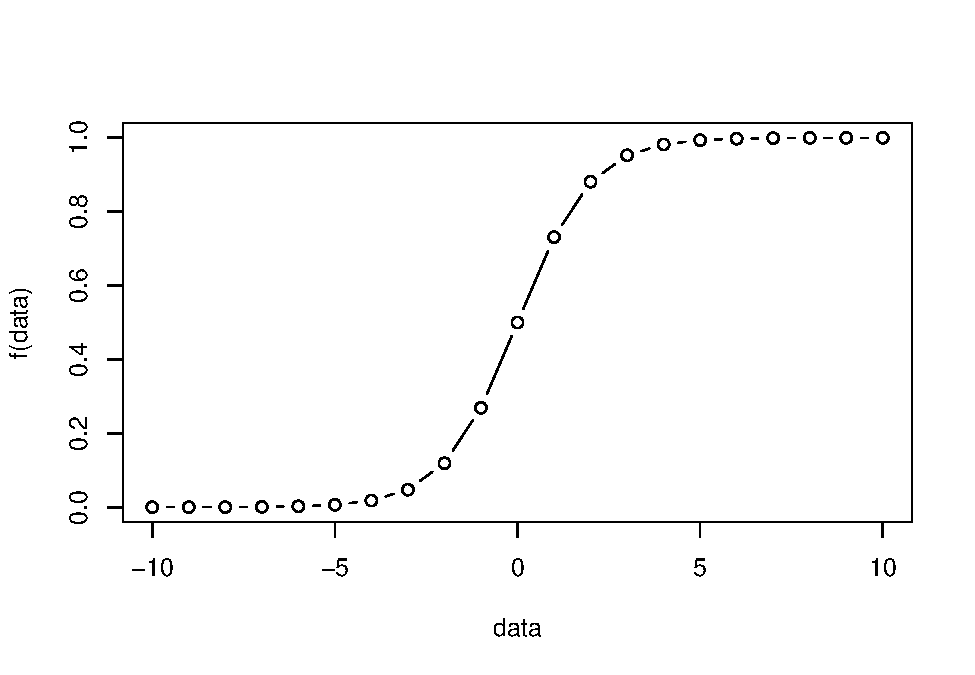
\includegraphics{bookdown-demo_files/figure-latex/unnamed-chunk-1-1.pdf}

We can also write the function into another format as follows:
\[log \frac{p(y=1)}{1-p(y=1)}= \beta_0+\beta_1x_1+...+\beta_nx_n\] Thus,
we know that the regression coeficients of \(\beta_i\) actually change
the ``log-odds'' of the event. Of course, note that the magnitude of
\(\beta_i\) is dependent upon the units of \(x_i\).

The following is an example testing whether that home teams are more
likely to win in NFL games. The results show that the odd of winning is
the same for both home and away teams.

\begin{Shaded}
\begin{Highlighting}[]
\NormalTok{mydata =}\StringTok{ }\KeywordTok{read.csv}\NormalTok{(}\KeywordTok{url}\NormalTok{(}\StringTok{'https://raw.githubusercontent.com/nfl-football-ops/Big-Data-Bowl/master/Data/games.csv'}\NormalTok{))}
\NormalTok{mydata}\OperatorTok{$}\NormalTok{result_new<-}\KeywordTok{ifelse}\NormalTok{(mydata}\OperatorTok{$}\NormalTok{HomeScore}\OperatorTok{>}\NormalTok{mydata}\OperatorTok{$}\NormalTok{VisitorScore,}\DecValTok{1}\NormalTok{,}\DecValTok{0}\NormalTok{)}
\KeywordTok{summary}\NormalTok{(mydata}\OperatorTok{$}\NormalTok{result_new)}
\end{Highlighting}
\end{Shaded}

\begin{verbatim}
##    Min. 1st Qu.  Median    Mean 3rd Qu.    Max. 
##  0.0000  0.0000  0.0000  0.4945  1.0000  1.0000
\end{verbatim}

\begin{Shaded}
\begin{Highlighting}[]
\NormalTok{mylogit1 =}\StringTok{ }\KeywordTok{glm}\NormalTok{(result_new}\OperatorTok{~}\DecValTok{1}\NormalTok{, }\DataTypeTok{family=}\NormalTok{binomial, }\DataTypeTok{data=}\NormalTok{mydata)}
\KeywordTok{summary}\NormalTok{(mylogit1)}
\end{Highlighting}
\end{Shaded}

\begin{verbatim}
## 
## Call:
## glm(formula = result_new ~ 1, family = binomial, data = mydata)
## 
## Deviance Residuals: 
##    Min      1Q  Median      3Q     Max  
## -1.168  -1.168  -1.168   1.187   1.187  
## 
## Coefficients:
##             Estimate Std. Error z value Pr(>|z|)
## (Intercept) -0.02198    0.20967  -0.105    0.917
## 
## (Dispersion parameter for binomial family taken to be 1)
## 
##     Null deviance: 126.14  on 90  degrees of freedom
## Residual deviance: 126.14  on 90  degrees of freedom
## AIC: 128.14
## 
## Number of Fisher Scoring iterations: 3
\end{verbatim}

\section{Probit}\label{probit}

As noted above, logit \(f(x)=log(\frac{p(y=1)}{1-p(y=1)})\) provides the
resulting range of \((0,1)\). Another way to provide the same rage is
through the cdf of normal distribution.The following R code is used to
illusrate this process.

\begin{Shaded}
\begin{Highlighting}[]
\NormalTok{data2<-}\KeywordTok{seq}\NormalTok{(}\OperatorTok{-}\DecValTok{5}\NormalTok{,}\DecValTok{5}\NormalTok{,}\DecValTok{1}\NormalTok{)}
\KeywordTok{plot}\NormalTok{(data2,}\KeywordTok{pnorm}\NormalTok{(data2),}\DataTypeTok{type =} \StringTok{"b"}\NormalTok{)}
\end{Highlighting}
\end{Shaded}

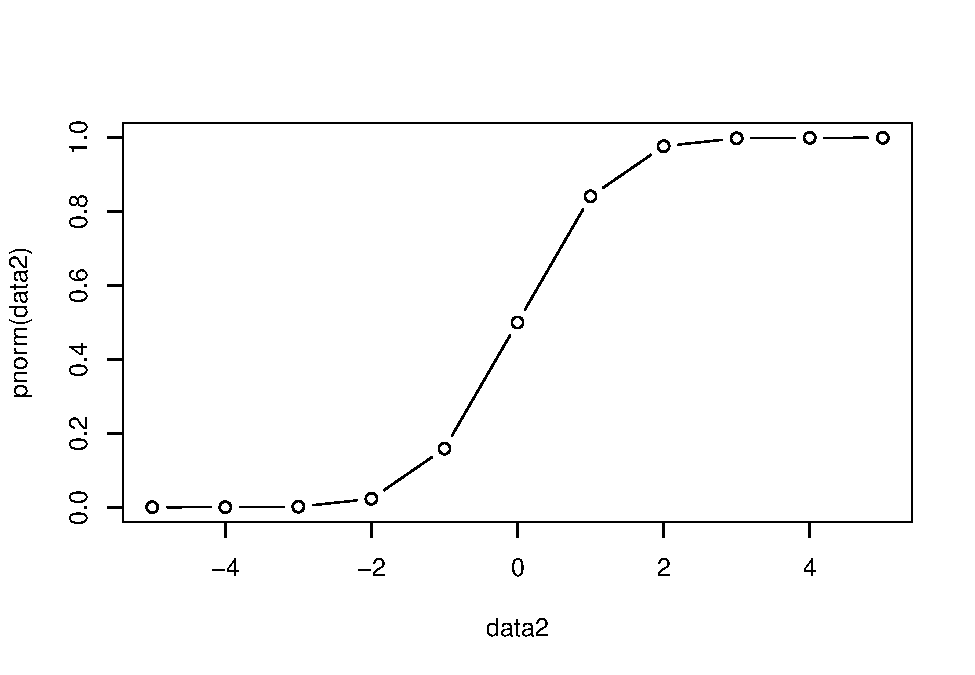
\includegraphics{bookdown-demo_files/figure-latex/unnamed-chunk-3-1.pdf}
Thus, the cdf of normal distribution can be used to indicate the
probability of \(p(y=1)\).

\[\Phi(\beta_0+\beta_1x_1+...+\beta_nx_n )= p(y=1)\]

Similar to logit model, we can also write the inverse function of the
cdf to get the function that can be from \(-\infty\) to \(+\infty\).

\[\beta_0+\beta_1x_1+...+\beta_nx_n =\Phi^{-1}(p(y=1))\]

Thus, for example, if \(X\beta\) = -2, based on
\(\Phi(\beta_0+\beta_1x_1+...+\beta_nx_n )= p(y=1)\) we can get that the
\(p(y=1)=0.023\).

In contrast, if \(X\beta\) = 3, the \(p(y=1)=0.999\).

\begin{Shaded}
\begin{Highlighting}[]
\KeywordTok{pnorm}\NormalTok{(}\OperatorTok{-}\DecValTok{2}\NormalTok{)}
\end{Highlighting}
\end{Shaded}

\begin{verbatim}
## [1] 0.02275013
\end{verbatim}

\begin{Shaded}
\begin{Highlighting}[]
\KeywordTok{pnorm}\NormalTok{(}\DecValTok{3}\NormalTok{)}
\end{Highlighting}
\end{Shaded}

\begin{verbatim}
## [1] 0.9986501
\end{verbatim}

Let's assume that there is a latent variable called \(Y^*\) such that

\[Y^*=X\beta+\epsilon, \epsilon \sim N(0,\sigma^2)\] You could think of
\(Y^*\) as a kind of ``proxy'' between \(X\beta+\epsilon\) and the
observed \(Y (1 or 0)\). Thus, we can get the following. Note that, it
does not have to be zero, and can be any constant.

\[
Y^*=\begin{cases} 0 \;\;\: if \;  y_i^* \leq 0 \\ 1 \;\;\: if \;  y_i^* > 0 \end{cases}
\]

Thus,

\[y_i^* > 0 \Rightarrow \beta^{'}X_i + \epsilon_i >0 \Rightarrow \epsilon_i > -\beta^{'}X_i\]

Thus, we can write it as follows. Note that
\(\frac{ \epsilon_i}{\sigma} \sim N(0,1)\)

\[p(y=1|x_i)= p(y_i^* >0|x_i)=p(\epsilon_i > -\beta^{'}X_i)= p(\frac{ \epsilon_i}{\sigma}>\frac{-\beta^{'}X_i}{\sigma})=\Phi(\frac{\beta^{'}X_i}{\sigma}) \]
We thus can get:

\[p(y=0|x_i)=1-\Phi(\frac{\beta^{'}X_i}{\sigma})\]

For \(p(y=1|x_i)=\Phi(\frac{\beta^{'}X_i}{\sigma})\), we can not really
estimate both \(\beta\) and \(\sigma\) as they are in a ratio. We can
assume \(\sigma =1\), then \(\epsilon \sim N(0,1)\). We know \(y_i\) and
\(x_i\) since we observe them. Thus, we can write it as follows.

\[p(y=1|x_i)=\Phi(\beta^{'}X_i)\]

\chapter{MLE}\label{intro}

\section{Basic idea of MLE}\label{basic-idea-of-mle}

Suppose that we flip a coin, \(y_i=0\) for tails and \(y_i=1\) for
heads. If we get \(p\) heads from \(n\) trials, we can get the
proportion of heads is \(p/n\), which is the sample mean. If we do not
do any further calculation, this is our best guess.

Suppose that the true proablity is \(\rho\), then we can get:

\[
\mathbf{L}(y_i)=\begin{cases} \rho \;\;\:   y_i = 1 \\ 1-\rho \;\;\:  y_i = 0 \end{cases}
\] Thus, we can also write it as follows.
\[\mathbf{L}(y_i) = \rho^{y_i}(1-\rho)^{1-y_i}\]

Thus, we can get:

\[\prod \mathbf{L}(y_i|\rho)=\rho^{\sum y_i}(1-\rho)^{\sum(1-y_i)}\]
Further, we can get a log-transformed format.

\[log (\prod \mathbf{L}(y_i|\rho))=\sum y_i log \rho + \sum(1-y_i) log(1-\rho)\]

To maximize the log-function above, we can calculate the derivative with
respect to \(\rho\).
\[\frac{\partial log (\prod \mathbf{L}(y_i|\rho)) }{\partial \rho}=\sum y_i \frac{1}{\rho}-\sum(1-y_i) \frac{1}{1-\rho}\]
Set the derivative to zero and solve for \(\rho\), we can get

\[\sum y_i \frac{1}{\rho}-\sum(1-y_i) \frac{1}{1-\rho}=0\]
\[\Rightarrow (1-\rho)\sum y_i - \rho \sum(1-y_i) =0\]
\[\Rightarrow \sum y_i-\rho\sum y_i - n\rho +\rho\sum y_i =0\]
\[\Rightarrow \sum y_i - n\rho  =0\]
\[\Rightarrow \rho  = \frac{\sum y_i}{n}=\frac{p}{n}\] Thus, we can see
that the \(\rho\) maximizing the likelihood function is equal to the
sample mean.

\section{Coin flip example, probit, and
logit}\label{coin-flip-example-probit-and-logit}

In the example above, we are not really trying to estimate a lot of
regression coefficients. What we are doing actually is to calculate the
sample mean, or intercept in the regresion sense. What does it mean?
Let's use some data to explain it.

Suppose that we flip a coin 20 times and observe 8 heads. We can use the
R's glm function to esimate the \(\rho\). If the result is consistent
with what we did above, we should observe that the \(cdf\) of the
esimate of \(\beta_0\) (i.e., intercept) should be equal to
\(8/20=0.4\).

\begin{Shaded}
\begin{Highlighting}[]
\NormalTok{coins<-}\KeywordTok{c}\NormalTok{(}\KeywordTok{rep}\NormalTok{(}\DecValTok{1}\NormalTok{,}\DataTypeTok{times=}\DecValTok{8}\NormalTok{),}\KeywordTok{rep}\NormalTok{(}\DecValTok{0}\NormalTok{,}\DataTypeTok{times=}\DecValTok{12}\NormalTok{))}
\KeywordTok{table}\NormalTok{(coins)}
\end{Highlighting}
\end{Shaded}

\begin{verbatim}
## coins
##  0  1 
## 12  8
\end{verbatim}

\begin{Shaded}
\begin{Highlighting}[]
\NormalTok{coins<-}\KeywordTok{as.data.frame}\NormalTok{(coins)}
\end{Highlighting}
\end{Shaded}

\subsection{Probit}\label{probit-1}

\begin{Shaded}
\begin{Highlighting}[]
\NormalTok{probitresults <-}\StringTok{ }\KeywordTok{glm}\NormalTok{(coins }\OperatorTok{~}\StringTok{ }\DecValTok{1}\NormalTok{, }\DataTypeTok{family =} \KeywordTok{binomial}\NormalTok{(}\DataTypeTok{link =} \StringTok{"probit"}\NormalTok{), }\DataTypeTok{data =}\NormalTok{ coins)}
\NormalTok{probitresults}
\end{Highlighting}
\end{Shaded}

\begin{verbatim}
## 
## Call:  glm(formula = coins ~ 1, family = binomial(link = "probit"), 
##     data = coins)
## 
## Coefficients:
## (Intercept)  
##     -0.2533  
## 
## Degrees of Freedom: 19 Total (i.e. Null);  19 Residual
## Null Deviance:       26.92 
## Residual Deviance: 26.92     AIC: 28.92
\end{verbatim}

\begin{Shaded}
\begin{Highlighting}[]
\KeywordTok{pnorm}\NormalTok{(probitresults}\OperatorTok{$}\NormalTok{coefficients)}
\end{Highlighting}
\end{Shaded}

\begin{verbatim}
## (Intercept) 
##         0.4
\end{verbatim}

As we can see the intercept is \(-0.2533\), and thus
\(\Phi(-0.2533471)=0.4\)

\subsection{Logit}\label{logit-1}

We can also use logit link to calculate the intercept as well. Recall
that

\[p(y=1)=\frac{1}{1+e^{-(\beta_0+\beta_1x_1+...+\beta_nx_n)}}=\frac{e^{\beta_0+\beta_1x_1+...+\beta_nx_n}}{1+e^{\beta_0+\beta_1x_1+...+\beta_nx_n}}\]
Thus,

\[p(y=1)=\frac{e^{\beta_0}}{1+e^{\beta_0}}\]

\begin{Shaded}
\begin{Highlighting}[]
\NormalTok{logitresults <-}\StringTok{ }\KeywordTok{glm}\NormalTok{(coins }\OperatorTok{~}\StringTok{ }\DecValTok{1}\NormalTok{, }\DataTypeTok{family =} \KeywordTok{binomial}\NormalTok{(}\DataTypeTok{link =} \StringTok{"logit"}\NormalTok{), }\DataTypeTok{data =}\NormalTok{ coins)}
\NormalTok{logitresults}\OperatorTok{$}\NormalTok{coefficients}
\end{Highlighting}
\end{Shaded}

\begin{verbatim}
## (Intercept) 
##  -0.4054651
\end{verbatim}

\begin{Shaded}
\begin{Highlighting}[]
\KeywordTok{exp}\NormalTok{(logitresults}\OperatorTok{$}\NormalTok{coefficients)}\OperatorTok{/}\NormalTok{(}\DecValTok{1}\OperatorTok{+}\KeywordTok{exp}\NormalTok{(logitresults}\OperatorTok{$}\NormalTok{coefficients))}
\end{Highlighting}
\end{Shaded}

\begin{verbatim}
## (Intercept) 
##         0.4
\end{verbatim}

Note that, the defaul link for the binomial in the glm function in
logit.

\section{Further on logit}\label{further-on-logit}

The probablity of \(y=1\) is as follows:

\[p=p(y=1)=\frac{1}{1+e^{-(\beta_0+\beta_1x_1+...+\beta_nx_n)}}=\frac{e^{\beta_0+\beta_1x_1+...+\beta_nx_n}}{1+e^{\beta_0+\beta_1x_1+...+\beta_nx_n}}\]

Thus, the likelihood function is as follows:

\[L=\prod p^{y_i}(1-p)^{1-y_i}=\prod (\frac{1}{1+e^{-(\beta_0+\beta_1x_1+...+\beta_nx_n)}})^{y_i}(\frac{1}{1+e^{\beta_0+\beta_1x_1+...+\beta_nx_n}})^{1-y_i}\]

\[=\prod (1+e^{-(\beta_0+\beta_1x_1+...+\beta_nx_n)})^{-y_i}(1+e^{\beta_0+\beta_1x_1+...+\beta_nx_n})^{-(1-y_i)}\]

Thus, the log-likelihood is as follows:
\[logL=\sum (-y_i \cdot log(1+e^{-(\beta_0+\beta_1x_1+...+\beta_nx_n)})-(1-y_i)\cdot log(1+e^{\beta_0+\beta_1x_1+...+\beta_nx_n}))\]

Typically, optimisers minimize a function, so we use negative
log-likelihood as minimising that is equivalent to maximising the
log-likelihood or the likelihood itself.

\begin{Shaded}
\begin{Highlighting}[]
\CommentTok{#Source of R code: https://www.r-bloggers.com/logistic-regression/}

\NormalTok{mle.logreg =}\StringTok{ }\ControlFlowTok{function}\NormalTok{(fmla, data)}
\NormalTok{\{}
  \CommentTok{# Define the negative log likelihood function}
\NormalTok{  logl <-}\StringTok{ }\ControlFlowTok{function}\NormalTok{(theta,x,y)\{}
\NormalTok{    y <-}\StringTok{ }\NormalTok{y}
\NormalTok{    x <-}\StringTok{ }\KeywordTok{as.matrix}\NormalTok{(x)}
\NormalTok{    beta <-}\StringTok{ }\NormalTok{theta[}\DecValTok{1}\OperatorTok{:}\KeywordTok{ncol}\NormalTok{(x)]}
    
    \CommentTok{# Use the log-likelihood of the Bernouilli distribution, where p is}
    \CommentTok{# defined as the logistic transformation of a linear combination}
    \CommentTok{# of predictors, according to logit(p)=(x%*%beta)}
\NormalTok{    loglik <-}\StringTok{ }\KeywordTok{sum}\NormalTok{(}\OperatorTok{-}\NormalTok{y}\OperatorTok{*}\KeywordTok{log}\NormalTok{(}\DecValTok{1} \OperatorTok{+}\StringTok{ }\KeywordTok{exp}\NormalTok{(}\OperatorTok{-}\NormalTok{(x}\OperatorTok\NormalTok{beta))) }\OperatorTok{-}\StringTok{ }\NormalTok{(}\DecValTok{1}\OperatorTok{-}\NormalTok{y)}\OperatorTok{*}\KeywordTok{log}\NormalTok{(}\DecValTok{1} \OperatorTok{+}\StringTok{ }\KeywordTok{exp}\NormalTok{(x}\OperatorTok\NormalTok{beta)))}
    \KeywordTok{return}\NormalTok{(}\OperatorTok{-}\NormalTok{loglik)}
\NormalTok{  \}}
  
  \CommentTok{# Prepare the data}
\NormalTok{  outcome =}\StringTok{ }\KeywordTok{rownames}\NormalTok{(}\KeywordTok{attr}\NormalTok{(}\KeywordTok{terms}\NormalTok{(fmla),}\StringTok{"factors"}\NormalTok{))[}\DecValTok{1}\NormalTok{]}
\NormalTok{  dfrTmp =}\StringTok{ }\KeywordTok{model.frame}\NormalTok{(data)}
\NormalTok{  x =}\StringTok{ }\KeywordTok{as.matrix}\NormalTok{(}\KeywordTok{model.matrix}\NormalTok{(fmla, }\DataTypeTok{data=}\NormalTok{dfrTmp))}
\NormalTok{  y =}\StringTok{ }\KeywordTok{as.numeric}\NormalTok{(}\KeywordTok{as.matrix}\NormalTok{(data[,}\KeywordTok{match}\NormalTok{(outcome,}\KeywordTok{colnames}\NormalTok{(data))]))}
  
  \CommentTok{# Define initial values for the parameters}
\NormalTok{  theta.start =}\StringTok{ }\KeywordTok{rep}\NormalTok{(}\DecValTok{0}\NormalTok{,(}\KeywordTok{dim}\NormalTok{(x)[}\DecValTok{2}\NormalTok{]))}
  \KeywordTok{names}\NormalTok{(theta.start) =}\StringTok{ }\KeywordTok{colnames}\NormalTok{(x)}
  
  \CommentTok{# Calculate the maximum likelihood}
\NormalTok{  mle =}\StringTok{ }\KeywordTok{optim}\NormalTok{(theta.start,logl,}\DataTypeTok{x=}\NormalTok{x,}\DataTypeTok{y=}\NormalTok{y, }\DataTypeTok{method =} \StringTok{'BFGS'}\NormalTok{, }\DataTypeTok{hessian=}\NormalTok{T)}
\NormalTok{  out =}\StringTok{ }\KeywordTok{list}\NormalTok{(}\DataTypeTok{beta=}\NormalTok{mle}\OperatorTok{$}\NormalTok{par,}\DataTypeTok{vcov=}\KeywordTok{solve}\NormalTok{(mle}\OperatorTok{$}\NormalTok{hessian),}\DataTypeTok{ll=}\DecValTok{2}\OperatorTok{*}\NormalTok{mle}\OperatorTok{$}\NormalTok{value)}
\NormalTok{\}}
\end{Highlighting}
\end{Shaded}

\begin{Shaded}
\begin{Highlighting}[]
\NormalTok{mydata =}\StringTok{ }\KeywordTok{read.csv}\NormalTok{(}\KeywordTok{url}\NormalTok{(}\StringTok{'https://stats.idre.ucla.edu/stat/data/binary.csv'}\NormalTok{))}
\NormalTok{mylogit1 =}\StringTok{ }\KeywordTok{glm}\NormalTok{(admit}\OperatorTok{~}\NormalTok{gre}\OperatorTok{+}\NormalTok{gpa}\OperatorTok{+}\KeywordTok{as.factor}\NormalTok{(rank), }\DataTypeTok{family=}\NormalTok{binomial, }\DataTypeTok{data=}\NormalTok{mydata)}

\NormalTok{mydata}\OperatorTok{$}\NormalTok{rank =}\StringTok{ }\KeywordTok{factor}\NormalTok{(mydata}\OperatorTok{$}\NormalTok{rank) }\CommentTok{#Treat rank as a categorical variable}
\NormalTok{fmla =}\StringTok{ }\KeywordTok{as.formula}\NormalTok{(}\StringTok{"admit~gre+gpa+rank"}\NormalTok{) }\CommentTok{#Create model formula}
\NormalTok{mylogit2 =}\StringTok{ }\KeywordTok{mle.logreg}\NormalTok{(fmla, mydata) }\CommentTok{#Estimate coefficients}


 \KeywordTok{print}\NormalTok{(}\KeywordTok{cbind}\NormalTok{(}\KeywordTok{coef}\NormalTok{(mylogit1), mylogit2}\OperatorTok{$}\NormalTok{beta))}
\end{Highlighting}
\end{Shaded}

\begin{verbatim}
##                          [,1]         [,2]
## (Intercept)      -3.989979073 -3.772676422
## gre               0.002264426  0.001375522
## gpa               0.804037549  0.898201239
## as.factor(rank)2 -0.675442928 -0.675543009
## as.factor(rank)3 -1.340203916 -1.356554831
## as.factor(rank)4 -1.551463677 -1.563396035
\end{verbatim}

\section{References}\label{references}

\url{http://www.columbia.edu/~so33/SusDev/Lecture_9.pdf}

\chapter{Linear Mixed Models}\label{linear-mixed-models}

\section{LM and GLM}\label{lm-and-glm}

Before moving to LMM, I would like to review LM and GLM first.

\subsection{LM}\label{lm}

\[Y|X \sim N(\mu(X),\sigma^2 I)\]

\[E(Y|X)=\mu(X)=X^T \beta\]

where,

\(\mu(X): random component\)

\(X^T \beta: covariates\)

\subsection{GLM-Definition}\label{glm-definition}

Ref:
\url{https://ocw.mit.edu/courses/mathematics/18-650-statistics-for-applications-fall-2016/lecture-slides/MIT18_650F16_GLM.pdf}

\[Y \sim exponential family\] Link function

\[g(\mu(X))=X^T \beta\]

\subsection{GLM-log link example}\label{glm-log-link-example}

\[\mu_i = \gamma e^{\delta t_i}\] Link function is log link, and it
becomes:

\[log(\mu_i) = log(\gamma) + log(\delta t_i)=\beta_0+\beta_1 t_i\] (This
is somehow similar to Poisson distribution.)

\subsection{GLM-Reciprocal link:}\label{glm-reciprocal-link}

\[\mu_i=\frac{\alpha x_i}{h+x_i}\]

Reciprocal link:

\[g(\mu_i)=\frac{1}{\mu_i}=\frac{1}{\alpha}+\frac{h}{\alpha}\frac{1}{x_i}=\beta_0+\beta_1 \frac{1}{x_i}\]

\subsection{GLM-exponential family:}\label{glm-exponential-family}

In a more general sense, for exponential family:

\[\begin{aligned} P_{\theta}(X)=P(X, \theta)&= e^{\sum \eta_i(\theta)T_i(X)} C(\theta)h(x)\\ &=e^{\sum \eta_i(\theta)T_i(X)} e^{-log(\frac{1}{c(\theta)})}h(x) \\ &= e^{\sum \eta_i(\theta)T_i(X)-log(\frac{1}{c(\theta)})} h(x)  \\&= e^{\sum \eta_i(\theta)T_i(X)-B(\theta)} h(x) \end{aligned}\]
\textbf{Normal distribution}

For normal distributions, it belongs to exponential family.

\[\begin{aligned} P_{\theta}(X) &= \frac{1}{\sigma\sqrt{2\pi}} e^{-\frac{1}{2}\frac{(x-\mu)^2}{\sigma^2}}\\ &=e^{-\frac{1}{2}\frac{(x-\mu)^2}{\sigma^2}} e^{log(\frac{1}{\sigma\sqrt{2\pi}})} \\ &= e^{-\frac{1}{2}\frac{(x-\mu)^2}{\sigma^2}-log (\sigma\sqrt{2\pi})} \\ &= e^{-\frac{1}{2\sigma^2}x^2-\frac{1}{2\sigma^2} \mu^2+\frac{x\mu}{\sigma^2}-log(\sqrt{2\pi}\sigma)}\\ &=e^{-\frac{1}{2\sigma^2}x^2+\frac{x\mu}{\sigma^2}-(\frac{1}{2\sigma^2} \mu^2+log(\sqrt{2\pi}\sigma))} \end{aligned}\]
Where,

\(\eta_1 =-\frac{1}{2\sigma^2}\) and \(T_1(x)=x^2\)

\(\eta_2 =-\frac{\mu}{\sigma^2}\) and \(T_2(x)=x\)

\(B(\theta)=\frac{1}{2\sigma^2} \mu^2+log(\sqrt{2\pi}\sigma)\)

\(h(x)=1\)

In the case above, \(\theta=(\mu, \sigma^2)\). If \(\sigma^2\) is known,
\(\theta=\mu\). In this case, we can rewrite the normal pdf as follows.

\[\begin{aligned} P_{\theta}(X) &=e^{-\frac{1}{2\sigma^2}x^2-\frac{1}{2\sigma^2} \mu^2+\frac{x\mu}{\sigma^2}-log(\sqrt{2\pi}\sigma)}\\ &=e^{\frac{x\mu}{\sigma^2}-\frac{1}{2\sigma^2} \mu^2}e^{-\frac{1}{2\sigma^2}x^2-log(\sqrt{2\pi}\sigma)} \end{aligned}\]
Where,

\(\eta_1 =-\frac{\mu}{\sigma^2}\) and \(T_1(x)=x\)

\(B(\theta)=\frac{1}{2\sigma^2} \mu^2\)

\(\begin{aligned} h(x) &=e^{-\frac{1}{2\sigma^2}x^2-log(\sqrt{2\pi}\sigma)} \\&=\frac{1}{\sigma\sqrt{2\pi}}e^{-\frac{1}{2}\frac{x^2}{\sigma^2}} \end{aligned}\)

Thus, we can see that \(h(x)\) is a normal pdf \(\sim N(0, \sigma^2)\).

\textbf{Bernoulli}

Another example, \(x\) is descrete. For example, Bernoulli:

\[ \begin{aligned} &= p^x(1-p)^{1-x}  \\ &=e^{log(p^x(1-p)^{1-x})} \\ &= e^{xlog(p)+(1-x)log(1-p)}\\ &= e^{xlog(p)-xlog(1-p)+log(1-p)}\\ &=e^{xlog(\frac{p}{1-p})+log(1-p)} \end{aligned}\]

Where,

\(\eta_1 =log(\frac{p}{1-p})\) and \(T_1(x)=x\)

\(B(\theta)=log(\frac{1}{1-p})\)

\(h(x) =1\)

\subsection{Canonical exponential
family}\label{canonical-exponential-family}

Canonical exponential family:

\[f_{\theta}(x)=e^{\frac{x\theta-b(\theta)}{\phi}+c(x,\phi)}\] where,
\(b(.)\) and \(c(.,.)\) are known.

\textbf{Normal distribution}

Again, use the normal pdf:

\[\begin{aligned} P_{\theta}(X) &= \frac{1}{\sigma\sqrt{2\pi}} e^{-\frac{1}{2}\frac{(x-\mu)^2}{\sigma^2}}\\ &=e^{-\frac{1}{2}\frac{(x-\mu)^2}{\sigma^2}} e^{log(\frac{1}{\sigma\sqrt{2\pi}})} \\ &= e^{-\frac{1}{2}\frac{(x-\mu)^2}{\sigma^2}-log (\sigma\sqrt{2\pi})} \\ &= e^{-\frac{1}{2\sigma^2}x^2-\frac{1}{2\sigma^2} \mu^2+\frac{x\mu}{\sigma^2}-log(\sqrt{2\pi}\sigma)}\\ &= e^{\frac{x\mu}{\sigma^2}-\frac{\mu^2}{2\sigma^2}+(-\frac{1}{2\sigma^2}x^2-log(\sqrt{2\pi}\sigma)) } \\ &=e^{\frac{x\mu-\frac{1}{2}\mu^2}{\sigma^2}+(-\frac{1}{2\sigma^2}x^2-log(\sqrt{2\pi}\sigma)) } \end{aligned}\]

Where (we assume \(\sigma^2\) is known.),

\(\theta=\mu\)

\(\phi =\sigma^2\)

\(b(\theta)=\frac{1}{2}\theta^2\)

\(\begin{aligned} c(x, \phi) &=-\frac{1}{2\sigma^2}x^2-log(\sqrt{2\pi}\sigma) \\ &=-\frac{1}{2\sigma^2}x^2-\frac{1}{2}log(2\pi\sigma^2) \\ &=-\frac{1}{2}(\frac{x^2}{\sigma^2}+log(2\pi\sigma^2)) \\ &=-\frac{1}{2}(\frac{x^2}{\phi}+log(2\pi \phi)) \end{aligned}\)

\subsection{Canonical exponential family - Expected value and
variance}\label{canonical-exponential-family---expected-value-and-variance}

\textbf{First derivative}

Canonical exponential family:

\[f_{\theta}(x)=e^{\frac{x\theta-b(\theta)}{\phi}+c(x,\phi)}\]

log likelihood (only one observation) \[log f_{\theta}(x)\]

\[\begin{aligned} E[\frac{\partial (logf_{\theta}(X))}{\partial \theta} ] &=E[\frac{\frac{\partial f_{\theta}(X)}{\partial \theta}}{f_{\theta}(X)}] \\ &= \int \frac{\frac{\partial f_{\theta}(X)}{\partial \theta}}{f_{\theta}(X)} f_{\theta}(X) dx  \\ &= \int \frac{\partial f_{\theta}(X)}{\partial \theta} dx \\ &= \frac{\partial}{\partial \theta} \int f_{\theta}(X)dx \\ &= \frac{\partial 1}{\partial \theta} \\ &=0  \end{aligned}\]
\textbf{Second derivative}

Second derivative

\[\begin{aligned} E[\frac{\partial^2 (logf_{\theta}(X))}{\partial \theta^2} ] &=E[ \frac{\partial}{\partial \theta}(\frac{\frac{\partial f_{\theta}(X)}{\partial \theta}}{f_{\theta}(X)})] \\  
&=E[\frac{\frac{\partial^2 f_{\theta}(X)}{\partial \theta^2}f_{\theta}(X)-(\frac{\partial f_{\theta}(X)}{\partial \theta})^2}{f^2_{\theta}(X)}] \\ &= \int \frac{\frac{\partial^2 f_{\theta}(X)}{\partial \theta^2}f_{\theta}(X)-(\frac{\partial f_{\theta}(X)}{\partial \theta})^2}{f_{\theta}(X)}dx \\ &=\int (\frac{\partial^2 f_{\theta}(X)}{\partial \theta^2} - \frac{(\frac{\partial f_{\theta}(X)}{\partial \theta})^2}{f_{\theta}(X)})dx  \\ 
&= \int \frac{\partial^2 f_{\theta}(X)}{\partial \theta^2} dx -\int \frac{(\frac{\partial f_{\theta}(X)}{\partial \theta})^2}{f_{\theta}(X)}dx \\ 
&=\frac{\partial^2}{\partial \theta^2}\int f_{\theta}(X) dx -\int \frac{(\frac{\partial f_{\theta}(X)}{\partial \theta})^2}{f_{\theta}(X)}dx \\ 
&=0-\int \frac{(\frac{\partial f_{\theta}(X)}{\partial \theta})^2}{f_{\theta}(X)}dx \\
&=0-\int \frac{(\frac{\partial f_{\theta}(X)}{\partial \theta})^2}{(f_{\theta}(X))^2}f_{\theta}(x)dx \\ &= - E[(\frac{\frac{\partial f_{\theta}(X)}{\partial \theta}}{f_{\theta}(X)})^2]\\ &= -E[(\frac{\partial (logf_{\theta}(X))}{\partial \theta})^2] \end{aligned}\]

Based on the first derivative, we can get:

\[log(f_{\theta}(X))=\frac{X\theta-b(\theta)}{\phi}+c(X,\phi)\]
\[E[\frac{\partial (log(f_{\theta}(X)))}{\partial \theta}]= E[\frac{X-b^{'}(\theta)}{\phi}]=\frac{E(X)-b^{'}(\theta)}{\phi}=0\]
Thus, we can get,

\[E(X)=b^{'}(\theta)\]

For second derivative, from the calculation above, we know that,

\[\begin{aligned} E[\frac{\partial^2 (logf_{\theta}(X))}{\partial \theta^2}]&=-E[(\frac{\partial (logf_{\theta}(X))}{\partial \theta})^2] \\ &= -E[(\frac{X-b^{'}(\theta)}{\phi})^2]\\ &=-E[(\frac{X-E(X)}{\phi})^2] \\ &= -\frac{Var(X)}{\phi^2}\end{aligned}\]
At the same time,
\[\begin{aligned} E[\frac{\partial^2 (logf_{\theta}(X))}{\partial \theta^2}]&=E[\frac{\partial (\frac{X-b^{'}(\theta)}{\phi})}{\partial \theta}] \\ &= E[-\frac{b^{''}(\theta)}{\phi}]\\ &= - \frac{b^{''}(\theta)}{\phi} \end{aligned}\]
Thus,

\[Var(X)=b^{''}(\theta) \phi\]

\subsection{Expected value and variance - Possion
Example}\label{expected-value-and-variance---possion-example}

Example of possion distribution

\[P(\lambda)=\frac{\lambda^k e^{-\lambda}}{k!}\]

If we put \(k\) as \(y\), and \(\lambda\) as \(\mu\), we can get:

\[P(\mu)=\frac{\mu^y e^{-\mu}}{y!}\] Compare to,

\[f_{\theta}(y)=e^{\frac{y\theta-b(\theta)}{\phi}+c(y,\phi)}\]

We can write it as the exponential format:

\[\begin{aligned} P(\mu) &=\frac{\mu^y e^{-\mu}}{y!}  \\ &= e^{log(\mu^y)+log(e^{-\mu})-log(y!)} \\ &= e^{ylog(\mu)-\mu-log(y!)}\end{aligned}\]

We thus know that \(\theta=log(\mu)\). We can contintue to write the
equation above as follows.

\[=e^{y\theta-e^{\theta}-log(y!)}\]

Thus, we can get:

\[E(X)=\frac{\partial (e^{\theta})}{\partial \theta}=e^{\theta}=\mu\]
\[Var(X)=\frac{\partial^{''} (e^{\theta})}{\partial \theta^2} \phi=\frac{\partial^{''} (e^{\theta})}{\partial \theta^2}=\mu\]

\subsection{Canonical link}\label{canonical-link}

A link functin can link \(X^T \beta\) to the mean \(\mu\).

That is,

\[g(\mu)=X^T \beta \rightarrow \mu = g^{-1}(X^T \beta)\] We know that

\[\mu = b^{'}(\theta)\]

Thus,

\[ b^{'}(\theta)=g^{-1}(X^T \beta)\] Thus,

\[g=b^{' -1}(\theta)\]

\subsection{Canonical link -
Bernoulli}\label{canonical-link---bernoulli}

PMF of Bernoulli:

\[ \begin{aligned} &= p^y(1-p)^{1-y}  \\ &=e^{log(p^y(1-p)^{1-y})} \\ &= e^{ylog(p)+(1-y)log(1-p)}\\ &= e^{ylog(p)-ylog(1-p)+log(1-p)}\\ &=e^{ylog(\frac{p}{1-p})+log(1-p)} \end{aligned} \]
Copared to the following:

\[f_{\theta}(y)=e^{\frac{y\theta-b(\theta)}{\phi}+c(y,\phi)}\] We need
to change the format of Bernoulli:

\[\theta= log \frac{p}{1-p}\] Thus,
\[e^{\theta}=\frac{p}{1-p} \rightarrow p=\frac{e^{\theta}}{1+e^{\theta}} \]
After that, we can contintue the Bernoulli:

\[\begin{aligned} &= e^{y\theta+log(1-\frac{e^{\theta}}{1+e^{\theta}})} \\ &=e^{y\theta+log(\frac{1}{1+e^{\theta}})} \\ &=e^{y\theta-log(1+e^{\theta})} \end{aligned}\]

Where,

\[b(\theta)=log(1+e^{\theta})\]

We can then try to calculate the derivative:

\[b^{'}(\theta)=\frac{\partial (log(1+e^{\theta}))}{\partial \theta}=\frac{e^{\theta}}{1+e^{\theta}}\]
We know that

\[b^{'}(\theta)=\mu\] Thus, we can get

\[\mu=\frac{e^{\theta}}{1+e^{\theta}}\] We can then calculate the
inverse function:

\[\theta=log(\frac{\mu}{1-\mu})\] Thus,

\[g(\mu)=log(\frac{\mu}{1-\mu})=X^T \beta\]

\subsection{NR - Bernoulli}\label{nr---bernoulli}

We know that the PMF for Bernoulli:

\[\begin{aligned} &= p^y(1-p)^{1-y} \\  &=e^{y\theta-log(1+e^{\theta})} \\ &=e^{yx^T \beta-log(1+e^{x^T \beta})} \end{aligned}\]
Thus,

\[\ell(\beta|Y,X)=\sum_{i=1}^{n}(Y_iX_i^{T}\beta-log(1+e^{X_i^T \beta}))\]
Thus, teh gradient is:

\[\nabla_{\ell}(\beta)=\sum_{i=1}^{n}(Y_iX_i - \frac{e^{X_i^T \beta}}{1+e^{X_i^T \beta}})\]
The Hessian is:

\[H_{\ell}(\beta)=-\sum_{i=1}^{n}\frac{e^{X_i^T \beta}}{(1+e^{X_i^T \beta})^2}X_iX_i^T\]

Thus,

\[\beta^{k+1}=\beta^k-(H_{\ell}(\beta^k))^{-1}\nabla_{\ell}(\beta^k) \]

\subsection{Iteratively Re-weighted Least
Squares}\label{iteratively-re-weighted-least-squares}

\section{LMM}\label{lmm}

The following is a shortened version of Jonathan Rosenblatt's LMM
tutorial. \url{http://www.john-ros.com/Rcourse/lme.html}.

In addition, another reference is from Douglas Bates's R package
document.
\url{https://cran.r-project.org/web/packages/lme4/vignettes/lmer.pdf?fbclid=IwAR1nmmRP9A0BrhKdgBibNjM5acR_spTpXV8QlQGdmTWyQz3ZtV3LYn6kCbQ}

Assume that \(y\) is a function of \(x\) and \(u\), where \(x\) is the
fixed effect and \(u\) is the random effect. Thus, we can get,

\[y|x, u = x'\beta+z'u+\epsilon\]

For random effect, one example can be that you want to test the
treatment effect, and sample 8 observations from 4 groups. You measure
before and after the treatment. In this case, \(x\) represents the
treatment effect, whereas \(z\) represents the group effect (i.e.,
random effect). Note that, in this case, it reminds the paired t-test.
Remember in SPSS, why do we do paired t-test? Typically, it is the case
when we measure a subject (or, participant) twice. In this case, we can
consider each participant as an unit of random effect (rather than as
group in the last example.)

\section{Calculate mean}\label{calculate-mean}

The following code generates 4 numbers (\(N(0,10)\)) for 4 groups. Then,
replicate it within each group.That is, in the end, there are 8
observations.

Note that, in the following code, there are no ``independent
variables''. Both the linear model and mixed model are actually just
trying to calculate the mean. Note that
lmer(y\textasciitilde{}1+1\textbar{}groups) and
lmer(y\textasciitilde{}1\textbar{}groups) will generate the same
results.

\begin{Shaded}
\begin{Highlighting}[]
\KeywordTok{set.seed}\NormalTok{(}\DecValTok{123}\NormalTok{)}
\NormalTok{n.groups <-}\StringTok{ }\DecValTok{4} \CommentTok{# number of groups}
\NormalTok{n.repeats <-}\StringTok{ }\DecValTok{2} \CommentTok{# samples per group}
\CommentTok{#Generating index for observations belong to the same group}
\NormalTok{groups <-}\StringTok{ }\KeywordTok{as.factor}\NormalTok{(}\KeywordTok{rep}\NormalTok{(}\DecValTok{1}\OperatorTok{:}\NormalTok{n.groups, }\DataTypeTok{each=}\NormalTok{n.repeats))}
\NormalTok{n <-}\StringTok{ }\KeywordTok{length}\NormalTok{(groups)}
\CommentTok{#Generating 4 random numbers, assuming normal distribution}
\NormalTok{z0 <-}\StringTok{ }\KeywordTok{rnorm}\NormalTok{(n.groups, }\DecValTok{0}\NormalTok{, }\DecValTok{10}\NormalTok{) }
\NormalTok{z <-}\StringTok{ }\NormalTok{z0[}\KeywordTok{as.numeric}\NormalTok{(groups)] }\CommentTok{# generate and inspect random group effects}
\NormalTok{z}
\end{Highlighting}
\end{Shaded}

\begin{verbatim}
## [1] -5.6047565 -5.6047565 -2.3017749 -2.3017749 15.5870831 15.5870831  0.7050839
## [8]  0.7050839
\end{verbatim}

\begin{Shaded}
\begin{Highlighting}[]
\NormalTok{epsilon <-}\StringTok{ }\KeywordTok{rnorm}\NormalTok{(n,}\DecValTok{0}\NormalTok{,}\DecValTok{1}\NormalTok{) }\CommentTok{# generate measurement error}
\NormalTok{beta0 <-}\StringTok{ }\DecValTok{2} \CommentTok{# this is the actual parameter of interest! The global mean.}
\NormalTok{y <-}\StringTok{ }\NormalTok{beta0 }\OperatorTok{+}\StringTok{ }\NormalTok{z }\OperatorTok{+}\StringTok{ }\NormalTok{epsilon }\CommentTok{# sample from an LMM}

\CommentTok{# fit a linear model assuming independence}
\CommentTok{# i.e., assume that there is no "group things".}
\NormalTok{lm.}\DecValTok{5}\NormalTok{ <-}\StringTok{ }\KeywordTok{lm}\NormalTok{(y}\OperatorTok{~}\DecValTok{1}\NormalTok{)}

\CommentTok{# fit a mixed-model that deals with the group dependence}
\CommentTok{#install.packages("lme4")}
\KeywordTok{library}\NormalTok{(lme4)}
\NormalTok{lme.}\FloatTok{5.}\NormalTok{a <-}\StringTok{ }\KeywordTok{lmer}\NormalTok{(y}\OperatorTok{~}\DecValTok{1}\OperatorTok{+}\DecValTok{1}\OperatorTok{|}\NormalTok{groups) }
\NormalTok{lme.}\FloatTok{5.}\NormalTok{b <-}\StringTok{ }\KeywordTok{lmer}\NormalTok{(y}\OperatorTok{~}\DecValTok{1}\OperatorTok{|}\NormalTok{groups) }
\NormalTok{lm.}\DecValTok{5}
\end{Highlighting}
\end{Shaded}

\begin{verbatim}
## 
## Call:
## lm(formula = y ~ 1)
## 
## Coefficients:
## (Intercept)  
##       4.283
\end{verbatim}

\begin{Shaded}
\begin{Highlighting}[]
\NormalTok{lme.}\FloatTok{5.}\NormalTok{a }
\end{Highlighting}
\end{Shaded}

\begin{verbatim}
## Linear mixed model fit by REML ['lmerMod']
## Formula: y ~ 1 + 1 | groups
## REML criterion at convergence: 36.1666
## Random effects:
##  Groups   Name        Std.Dev.
##  groups   (Intercept) 8.8521  
##  Residual             0.8873  
## Number of obs: 8, groups:  groups, 4
## Fixed Effects:
## (Intercept)  
##       4.283
\end{verbatim}

\begin{Shaded}
\begin{Highlighting}[]
\NormalTok{lme.}\FloatTok{5.}\NormalTok{b }
\end{Highlighting}
\end{Shaded}

\begin{verbatim}
## Linear mixed model fit by REML ['lmerMod']
## Formula: y ~ 1 | groups
## REML criterion at convergence: 36.1666
## Random effects:
##  Groups   Name        Std.Dev.
##  groups   (Intercept) 8.8521  
##  Residual             0.8873  
## Number of obs: 8, groups:  groups, 4
## Fixed Effects:
## (Intercept)  
##       4.283
\end{verbatim}

\section{Test the treatment effect}\label{test-the-treatment-effect}

As we can see that, LLM and paired t-test generate the same t-value.

\begin{Shaded}
\begin{Highlighting}[]
\NormalTok{times<-}\KeywordTok{rep}\NormalTok{(}\KeywordTok{c}\NormalTok{(}\DecValTok{1}\NormalTok{,}\DecValTok{2}\NormalTok{),}\DecValTok{4}\NormalTok{) }\CommentTok{# first time and second time}
\NormalTok{times}
\end{Highlighting}
\end{Shaded}

\begin{verbatim}
## [1] 1 2 1 2 1 2 1 2
\end{verbatim}

\begin{Shaded}
\begin{Highlighting}[]
\NormalTok{data_combined<-}\KeywordTok{cbind}\NormalTok{(y,groups,times)}
\NormalTok{data_combined}
\end{Highlighting}
\end{Shaded}

\begin{verbatim}
##               y groups times
## [1,] -3.4754687      1     1
## [2,] -1.8896915      1     2
## [3,]  0.1591413      2     1
## [4,] -1.5668361      2     2
## [5,] 16.9002303      3     1
## [6,] 17.1414212      3     2
## [7,]  3.9291657      4     1
## [8,]  3.0648977      4     2
\end{verbatim}

\begin{Shaded}
\begin{Highlighting}[]
\NormalTok{lme_diff_times<-}\StringTok{ }\KeywordTok{lmer}\NormalTok{(y}\OperatorTok{~}\NormalTok{times}\OperatorTok{+}\NormalTok{(}\DecValTok{1}\OperatorTok{|}\NormalTok{groups)) }


\NormalTok{t_results<-}\KeywordTok{t.test}\NormalTok{(y}\OperatorTok{~}\NormalTok{times, }\DataTypeTok{paired=}\OtherTok{TRUE}\NormalTok{)}

\NormalTok{lme_diff_times}
\end{Highlighting}
\end{Shaded}

\begin{verbatim}
## Linear mixed model fit by REML ['lmerMod']
## Formula: y ~ times + (1 | groups)
## REML criterion at convergence: 35.0539
## Random effects:
##  Groups   Name        Std.Dev.
##  groups   (Intercept) 8.845   
##  Residual             1.013   
## Number of obs: 8, groups:  groups, 4
## Fixed Effects:
## (Intercept)        times  
##      4.5691      -0.1908
\end{verbatim}

\begin{Shaded}
\begin{Highlighting}[]
\KeywordTok{print}\NormalTok{(}\StringTok{"The following results are from paired t-test"}\NormalTok{)}
\end{Highlighting}
\end{Shaded}

\begin{verbatim}
## [1] "The following results are from paired t-test"
\end{verbatim}

\begin{Shaded}
\begin{Highlighting}[]
\NormalTok{t_results}\OperatorTok{$}\NormalTok{statistic}
\end{Highlighting}
\end{Shaded}

\begin{verbatim}
##         t 
## 0.2664793
\end{verbatim}

\section{Another example}\label{another-example}

\begin{Shaded}
\begin{Highlighting}[]
\KeywordTok{data}\NormalTok{(Dyestuff, }\DataTypeTok{package=}\StringTok{'lme4'}\NormalTok{)}
\KeywordTok{attach}\NormalTok{(Dyestuff)}
\end{Highlighting}
\end{Shaded}

\begin{verbatim}
## The following objects are masked from Dyestuff (pos = 7):
## 
##     Batch, Yield
\end{verbatim}

\begin{Shaded}
\begin{Highlighting}[]
\NormalTok{Dyestuff}
\end{Highlighting}
\end{Shaded}

\begin{verbatim}
##    Batch Yield
## 1      A  1545
## 2      A  1440
## 3      A  1440
## 4      A  1520
## 5      A  1580
## 6      B  1540
## 7      B  1555
## 8      B  1490
## 9      B  1560
## 10     B  1495
## 11     C  1595
## 12     C  1550
## 13     C  1605
## 14     C  1510
## 15     C  1560
## 16     D  1445
## 17     D  1440
## 18     D  1595
## 19     D  1465
## 20     D  1545
## 21     E  1595
## 22     E  1630
## 23     E  1515
## 24     E  1635
## 25     E  1625
## 26     F  1520
## 27     F  1455
## 28     F  1450
## 29     F  1480
## 30     F  1445
\end{verbatim}

\begin{Shaded}
\begin{Highlighting}[]
\NormalTok{lme_batch<-}\StringTok{ }\KeywordTok{lmer}\NormalTok{( Yield }\OperatorTok{~}\StringTok{ }\DecValTok{1} \OperatorTok{+}\StringTok{ }\NormalTok{(}\DecValTok{1}\OperatorTok{|}\NormalTok{Batch)  , Dyestuff )}
\KeywordTok{summary}\NormalTok{(lme_batch)}
\end{Highlighting}
\end{Shaded}

\begin{verbatim}
## Linear mixed model fit by REML ['lmerMod']
## Formula: Yield ~ 1 + (1 | Batch)
##    Data: Dyestuff
## 
## REML criterion at convergence: 319.7
## 
## Scaled residuals: 
##     Min      1Q  Median      3Q     Max 
## -1.4117 -0.7634  0.1418  0.7792  1.8296 
## 
## Random effects:
##  Groups   Name        Variance Std.Dev.
##  Batch    (Intercept) 1764     42.00   
##  Residual             2451     49.51   
## Number of obs: 30, groups:  Batch, 6
## 
## Fixed effects:
##             Estimate Std. Error t value
## (Intercept)  1527.50      19.38    78.8
\end{verbatim}

\section{Full LMM model}\label{full-lmm-model}

In the following, I used the data from the package of lme4. For Days +
(1 \textbar{} Subject), it only has random intercept; in contrast, Days
+ ( Days\textbar{} Subject ) has both random intercept and random slope
for Days. Note that, random effects do not generate specific slopes for
each level of Days, but rather just a variance of all the slopes.

Therefore, we can see that ``Days + ( Days\textbar{} Subject )'' and
``Days + ( 1+Days\textbar{} Subject )'' generate the same results. For
more discussion, you can refer to the following link:
\url{https://www.jaredknowles.com/journal/2013/11/25/getting-started-with-mixed-effect-models-in-r}

\begin{Shaded}
\begin{Highlighting}[]
\KeywordTok{data}\NormalTok{(sleepstudy, }\DataTypeTok{package=}\StringTok{'lme4'}\NormalTok{)}
\KeywordTok{attach}\NormalTok{(sleepstudy)}
\end{Highlighting}
\end{Shaded}

\begin{verbatim}
## The following objects are masked from sleepstudy (pos = 7):
## 
##     Days, Reaction, Subject
\end{verbatim}

\begin{Shaded}
\begin{Highlighting}[]
\NormalTok{fm1 <-}\StringTok{ }\KeywordTok{lmer}\NormalTok{(Reaction }\OperatorTok{~}\StringTok{ }\NormalTok{Days }\OperatorTok{+}\StringTok{ }\NormalTok{(}\DecValTok{1} \OperatorTok{|}\StringTok{ }\NormalTok{Subject), sleepstudy)}
\KeywordTok{summary}\NormalTok{(fm1)}
\end{Highlighting}
\end{Shaded}

\begin{verbatim}
## Linear mixed model fit by REML ['lmerMod']
## Formula: Reaction ~ Days + (1 | Subject)
##    Data: sleepstudy
## 
## REML criterion at convergence: 1786.5
## 
## Scaled residuals: 
##     Min      1Q  Median      3Q     Max 
## -3.2257 -0.5529  0.0109  0.5188  4.2506 
## 
## Random effects:
##  Groups   Name        Variance Std.Dev.
##  Subject  (Intercept) 1378.2   37.12   
##  Residual              960.5   30.99   
## Number of obs: 180, groups:  Subject, 18
## 
## Fixed effects:
##             Estimate Std. Error t value
## (Intercept) 251.4051     9.7467   25.79
## Days         10.4673     0.8042   13.02
## 
## Correlation of Fixed Effects:
##      (Intr)
## Days -0.371
\end{verbatim}

\begin{Shaded}
\begin{Highlighting}[]
\NormalTok{fm2<-}\KeywordTok{lmer}\NormalTok{ ( Reaction }\OperatorTok{~}\StringTok{ }\NormalTok{Days }\OperatorTok{+}\StringTok{ }\NormalTok{( Days}\OperatorTok{|}\StringTok{ }\NormalTok{Subject ) , }\DataTypeTok{data=}\NormalTok{ sleepstudy )}
\KeywordTok{summary}\NormalTok{(fm2)}
\end{Highlighting}
\end{Shaded}

\begin{verbatim}
## Linear mixed model fit by REML ['lmerMod']
## Formula: Reaction ~ Days + (Days | Subject)
##    Data: sleepstudy
## 
## REML criterion at convergence: 1743.6
## 
## Scaled residuals: 
##     Min      1Q  Median      3Q     Max 
## -3.9536 -0.4634  0.0231  0.4633  5.1793 
## 
## Random effects:
##  Groups   Name        Variance Std.Dev. Corr
##  Subject  (Intercept) 611.90   24.737       
##           Days         35.08    5.923   0.07
##  Residual             654.94   25.592       
## Number of obs: 180, groups:  Subject, 18
## 
## Fixed effects:
##             Estimate Std. Error t value
## (Intercept)  251.405      6.824  36.843
## Days          10.467      1.546   6.771
## 
## Correlation of Fixed Effects:
##      (Intr)
## Days -0.138
\end{verbatim}

\begin{Shaded}
\begin{Highlighting}[]
\NormalTok{fm3<-}\KeywordTok{lmer}\NormalTok{ ( Reaction }\OperatorTok{~}\StringTok{ }\NormalTok{Days }\OperatorTok{+}\StringTok{ }\NormalTok{(}\DecValTok{1}\OperatorTok{+}\NormalTok{Days}\OperatorTok{|}\StringTok{ }\NormalTok{Subject ) , }\DataTypeTok{data=}\NormalTok{ sleepstudy )}
\KeywordTok{summary}\NormalTok{(fm3)}
\end{Highlighting}
\end{Shaded}

\begin{verbatim}
## Linear mixed model fit by REML ['lmerMod']
## Formula: Reaction ~ Days + (1 + Days | Subject)
##    Data: sleepstudy
## 
## REML criterion at convergence: 1743.6
## 
## Scaled residuals: 
##     Min      1Q  Median      3Q     Max 
## -3.9536 -0.4634  0.0231  0.4633  5.1793 
## 
## Random effects:
##  Groups   Name        Variance Std.Dev. Corr
##  Subject  (Intercept) 611.90   24.737       
##           Days         35.08    5.923   0.07
##  Residual             654.94   25.592       
## Number of obs: 180, groups:  Subject, 18
## 
## Fixed effects:
##             Estimate Std. Error t value
## (Intercept)  251.405      6.824  36.843
## Days          10.467      1.546   6.771
## 
## Correlation of Fixed Effects:
##      (Intr)
## Days -0.138
\end{verbatim}

\section{Serial correlations in time and
space}\label{serial-correlations-in-time-and-space}

The hierarchical model of \(y|x, u = x'\beta+z'u+\epsilon\) can work
well for correlations within blocks, but not for correlations in time as
the correlations decay in time. The following uses nlme package to
calculate time serial data.

\begin{Shaded}
\begin{Highlighting}[]
\KeywordTok{library}\NormalTok{(nlme)}
\KeywordTok{head}\NormalTok{(nlme}\OperatorTok{::}\NormalTok{Ovary,}\DataTypeTok{n=}\DecValTok{50}\NormalTok{)}
\end{Highlighting}
\end{Shaded}

\begin{verbatim}
## Grouped Data: follicles ~ Time | Mare
##    Mare        Time follicles
## 1     1 -0.13636360        20
## 2     1 -0.09090910        15
## 3     1 -0.04545455        19
## 4     1  0.00000000        16
## 5     1  0.04545455        13
## 6     1  0.09090910        10
## 7     1  0.13636360        12
## 8     1  0.18181820        14
## 9     1  0.22727270        13
## 10    1  0.27272730        20
## 11    1  0.31818180        22
## 12    1  0.36363640        15
## 13    1  0.40909090        18
## 14    1  0.45454550        17
## 15    1  0.50000000        14
## 16    1  0.54545450        18
## 17    1  0.59090910        14
## 18    1  0.63636360        16
## 19    1  0.68181820        17
## 20    1  0.72727270        18
## 21    1  0.77272730        18
## 22    1  0.81818180        17
## 23    1  0.86363640        14
## 24    1  0.90909090        12
## 25    1  0.95454550        12
## 26    1  1.00000000        14
## 27    1  1.04545500        10
## 28    1  1.09090900        11
## 29    1  1.13636400        16
## 30    2 -0.15000000         6
## 31    2 -0.10000000         6
## 32    2 -0.05000000         8
## 33    2  0.00000000         7
## 34    2  0.05000000        16
## 35    2  0.10000000        10
## 36    2  0.15000000        13
## 37    2  0.20000000         9
## 38    2  0.25000000         7
## 39    2  0.30000000         6
## 40    2  0.35000000         8
## 41    2  0.40000000         8
## 42    2  0.45000000         6
## 43    2  0.50000000         8
## 44    2  0.55000000         7
## 45    2  0.60000000         9
## 46    2  0.65000000         6
## 47    2  0.70000000         4
## 48    2  0.75000000         5
## 49    2  0.80000000         8
## 50    2  0.85000000        11
\end{verbatim}

\begin{Shaded}
\begin{Highlighting}[]
\NormalTok{fm1Ovar.lme <-}\StringTok{ }\NormalTok{nlme}\OperatorTok{::}\KeywordTok{lme}\NormalTok{(}\DataTypeTok{fixed=}\NormalTok{follicles }\OperatorTok{~}\StringTok{ }\KeywordTok{sin}\NormalTok{(}\DecValTok{2}\OperatorTok{*}\NormalTok{pi}\OperatorTok{*}\NormalTok{Time) }\OperatorTok{+}\StringTok{ }\KeywordTok{cos}\NormalTok{(}\DecValTok{2}\OperatorTok{*}\NormalTok{pi}\OperatorTok{*}\NormalTok{Time), }
                   \DataTypeTok{data =}\NormalTok{ Ovary, }
                   \DataTypeTok{random =} \KeywordTok{pdDiag}\NormalTok{(}\OperatorTok{~}\KeywordTok{sin}\NormalTok{(}\DecValTok{2}\OperatorTok{*}\NormalTok{pi}\OperatorTok{*}\NormalTok{Time)), }
                   \DataTypeTok{correlation=}\KeywordTok{corAR1}\NormalTok{() )}
\KeywordTok{summary}\NormalTok{(fm1Ovar.lme)}
\end{Highlighting}
\end{Shaded}

\begin{verbatim}
## Linear mixed-effects model fit by REML
##  Data: Ovary 
##        AIC     BIC   logLik
##   1563.448 1589.49 -774.724
## 
## Random effects:
##  Formula: ~sin(2 * pi * Time) | Mare
##  Structure: Diagonal
##         (Intercept) sin(2 * pi * Time) Residual
## StdDev:    2.858385           1.257977 3.507053
## 
## Correlation Structure: AR(1)
##  Formula: ~1 | Mare 
##  Parameter estimate(s):
##       Phi 
## 0.5721866 
## Fixed effects: follicles ~ sin(2 * pi * Time) + cos(2 * pi * Time) 
##                        Value Std.Error  DF   t-value p-value
## (Intercept)        12.188089 0.9436602 295 12.915760  0.0000
## sin(2 * pi * Time) -2.985297 0.6055968 295 -4.929513  0.0000
## cos(2 * pi * Time) -0.877762 0.4777821 295 -1.837159  0.0672
##  Correlation: 
##                    (Intr) s(*p*T
## sin(2 * pi * Time)  0.000       
## cos(2 * pi * Time) -0.123  0.000
## 
## Standardized Within-Group Residuals:
##         Min          Q1         Med          Q3         Max 
## -2.34910093 -0.58969626 -0.04577893  0.52931186  3.37167486 
## 
## Number of Observations: 308
## Number of Groups: 11
\end{verbatim}

\chapter{Basic Stat Concepts}\label{basic-stat-concepts}

\section{Score}\label{score}

The score is the gradient (the vector of partial derivatives) of
\(log L(\theta)\), with respect to an m-dimensional parameter vector
\(\theta\).

\[S(\theta) = \frac{\partial\ell}{\partial \theta}\] Typically, they use
\(\nabla\) to denote the partical derivative.

\[\nabla \ell\]

Such differentiation will generate a \(m \times 1\) row vector, which
indicates the sensitivity of the likelihood.

Quote from Steffen Lauritzen's slides: ``Generally the solution to this
equation must be calculated by iterative methods. One of the most common
methods is the Newton--Raphson method and this is based on successive
approximations to the solution, using Taylor's theorem to approximate
the equation.''

For instance, using logit link, we can get the first derivative of log
likelihood logistic regression as follows. We can not really find
\(\beta\) easily to make the equation to be 0.

\[\begin{aligned}
\frac{\partial \ell} {\partial \beta} 
&= \sum_{i=1}^{n}x_i^T[y_i-\frac{e^{\beta^Tx_i}}{1+e^{\beta^Tx_i}}] \\
&=\sum_{i=1}^{n} x_i^T[y_i-\hat{y_i}]
\end{aligned}\]

\section{Gradient and Jacobian}\label{gradient-and-jacobian}

\textbf{Remarks}: This part discusses gradient in a more general sense.

When \(f(x)\) is only in a single dimension space:

\(\mathbb{R}^n \rightarrow \mathbb{R}\)

\[\nabla f(x)=[\frac{\partial f}{\partial x_1},\frac{\partial f}{\partial x_2},...,\frac{\partial f}{\partial x_n}]\]
When \(f(x)\) is only in a m-dimension space (i.e., Jacobian):
\(\mathbb{R}^n \rightarrow \mathbb{R^m}\)

\[Jac(f)=\begin{bmatrix}
\frac{\partial f_1}{\partial x_1} & \frac{\partial f_1}{\partial x_2} & \frac{\partial f_1}{\partial x_3} & ... & \frac{\partial f_1}{\partial x_n}\\
\frac{\partial f_2}{\partial x_1} & \frac{\partial f_2}{\partial x_2} & \frac{\partial f_2}{\partial x_3} & ... & \frac{\partial f_2}{\partial x_n} \\
...\\
\frac{\partial f_m}{\partial x_1} & \frac{\partial f_m}{\partial x_2} & \frac{\partial f_n}{\partial x_3} & ... & \frac{\partial f_m}{\partial x_n}
\end{bmatrix}\]

For instance,

\(\mathbb{R}^n \rightarrow \mathbb{R}\):

\[f(x,y)=x^2+2y\]
\[\nabla f(x,y)=[\frac{\partial f}{\partial x},\frac{\partial f}{\partial y}]=[2x,2]\]
\(\mathbb{R}^n \rightarrow \mathbb{R^m}\)

\[f(x,y)=(x^2+2y,x^3)\] \[Jac(f)=\begin{bmatrix}
2x & 2\\
2x^2 & 0 
\end{bmatrix}\]

\section{Hessian and Fisher
Information}\label{hessian-and-fisher-information}

Hessian matrix or Hessian is a square matrix of second-order partial
derivatives of a scalar-valued function, or scalar field.

\(\mathbb{R}^n \rightarrow \mathbb{R}\)

\[Hessian=\nabla ^2(f) =\begin{bmatrix}
\frac{\partial^2 f}{\partial x_1^2} & \frac{\partial^2 f}{\partial x_1 \partial x_2} & \frac{\partial^2 f}{\partial x_1 \partial x_3} & ... & \frac{\partial^2 f}{\partial x_1 \partial x_n}\\
\frac{\partial^2 f}{\partial x_2 \partial x_1} & \frac{\partial^2 f}{\partial x_2^2} & \frac{\partial^2 f}{\partial x_2 \partial x_3} & ... & \frac{\partial^2 f}{\partial x_2 \partial x_n} \\
\frac{\partial^2 f}{\partial x_3 \partial x_1} & \frac{\partial^2 f}{\partial x_3 \partial x_2} & \frac{\partial^2 f}{\partial x_3^2} & ... & \frac{\partial^2 f}{\partial x_3 \partial x_n} \\
...\\
\frac{\partial^2 f}{\partial x_n \partial x_1} & \frac{\partial^2 f}{\partial x_n \partial x_2} & \frac{\partial^2 f}{\partial x_n \partial x_3} & ... & \frac{\partial^2 f}{\partial x_n^2}
\end{bmatrix}\]

As a special case, in the context of logit:

Suppose that the log likelihood function is \(\ell (\theta)\).
\(\theta\) is a \(m\) demension vector.

\[ \theta = \begin{bmatrix}\theta_1 \\
\theta_2 \\
\theta_3 \\
\theta_4 \\
...\\
\theta_m \\
\end{bmatrix}\]

\[Hessian=\nabla ^2(\ell) =\begin{bmatrix}
\frac{\partial^2 \ell}{\partial \theta_1^2} & \frac{\partial^2 \ell}{\partial \theta_1 \partial \theta_2} & \frac{\partial^2 \ell}{\partial \theta_1 \partial \theta_3} & ... & \frac{\partial^2 \ell}{\partial \theta_1 \partial \theta_m}\\
\frac{\partial^2 \ell}{\partial \theta_2 \partial \theta_1} & \frac{\partial^2 \ell}{\partial \theta_2^2 } & \frac{\partial^2 \ell}{\partial \theta_1 \partial \theta_3} & ... & \frac{\partial^2 \ell}{\partial \theta_1 \partial \theta_m} \\
\frac{\partial^2 \ell}{\partial \theta_3 \partial \theta_1} & \frac{\partial^2 \ell}{\partial \theta_3 \theta_2 } & \frac{\partial^2 \ell}{\partial \theta_3^2} & ... & \frac{\partial^2 \ell}{\partial \theta_3 \partial \theta_m} \\
...\\
\frac{\partial^2 \ell}{\partial \theta_m \partial \theta_1} & \frac{\partial^2 \ell}{\partial \theta_m \theta_2 } & \frac{\partial^2 \ell}{\partial \theta_m \partial \theta_3} & ... & \frac{\partial^2 \ell}{\partial \theta_m \partial \theta_m} 
\end{bmatrix}\]

``In statistics, the observed information, or observed Fisher
information, is the negative of the second derivative (the Hessian
matrix) of the''log-likelihood" (the logarithm of the likelihood
function). It is a sample-based version of the Fisher information."
(Direct quote from Wikipedia.)

Thus, the observed information matrix:

\[-Hessian=-\nabla ^2(\ell) \]

Expected (Fisher) information matrix:

\[E[-\nabla ^2(\ell)] \]

\section{Canonical link function}\label{canonical-link-function}

Inspired by a Stack Exchange post, I created the following figure:

\[ \frac{Paramter}{\theta} \longrightarrow \gamma^{'}(\theta) = \mu \longrightarrow \frac{Mean}{\mu} \longrightarrow g(\mu) = \eta \longrightarrow \frac{ Linear predictor}{\eta} \]

For the case of \(n\) time Bernoulli (i.e., Binomial), its canonical
link function is logit. Specifically,

\[ \frac{Paramter}{\theta=\beta^Tx_i}  \longrightarrow \gamma^{'}(\theta)= \frac{e^{\beta^Tx_i}}{1+e^{\beta^Tx_i}}\longrightarrow \frac{Mean}{\mu=\frac{e^{\beta^Tx_i}}{1+e^{\beta^Tx_i}}}\longrightarrow g(\mu) = log \frac{\frac{e^{\beta^Tx_i}}{1+e^{\beta^Tx_i}}}{1-\frac{e^{\beta^Tx_i}}{1+e^{\beta^Tx_i}}}\longrightarrow \frac{ Linear predictor}{\eta = \beta^Tx_i}\]
Thus, we can see that,

\[\theta \equiv \eta \] The link function \(g(\mu)\) relates the linear
predictor \(\eta = \beta^Tx_i\) to the mean \(\mu\).

\textbf{Remarks}:

\begin{enumerate}
\def\labelenumi{(\arabic{enumi})}
\item
  Parameter is \(\theta = \beta ^T x_i\) (Not \(\mu\)!).
\item
  \(\mu=p(y=1)=\frac{e^{\beta^Tx_i}}{1+e^{\beta^Tx_i}}\) (Not logit!).
\item
  Link function (i.e., \(g(\mu)\)) = logit = logarithm of odds = log
  \(\frac{Event - Happened }{Event - Not - Happened}\).
\item
  \(g(\mu) = log \frac{\mu}{1-\mu}=\beta^T x_i\). Thus, link function =
  linear predictor = log odds!
\item
  Quote from the Stack Exchange post ``Newton Method and Fisher scoring
  for finding the ML estimator coincide, these links simplify the
  derivation of the MLE.''
\end{enumerate}

(Recall, we know that \(\mu\) or \(p(y=1)\) is the mean function. Recall
that, \(n\) trails of coin flips, and get \(p\) heads. Thus
\(\mu = \frac{p}{n}\).)

\section{Ordinary Least Squares (OLS)}\label{ordinary-least-squares-ols}

Suppose we have \(n\) observation, and \(m\) variables.

\[\begin{bmatrix}
x_{11} & x_{12} & x_{13} & ... & x_{1m}\\
x_{21} & x_{22} & x_{23} & ... & x_{2m} \\
...\\
x_{n1} & x_{n2} & x_{n3} & ... & x_{nm}
\end{bmatrix}\]

Thus, we can write it as the following \(n\) equations.

\[y_1=\beta_0+\beta_1 x_{11}+\beta_2 x_{12}+...+ \beta_m x_{1m}\]
\[y_2=\beta_0+\beta_1 x_{21}+\beta_2 x_{22}+...+ \beta_m x_{2m}\]
\[y_3=\beta_0+\beta_1 x_{31}+\beta_2 x_{32}+...+ \beta_m x_{3m}\]
\[...\]

\[y_n=\beta_0+\beta_1 x_{n1}+\beta_2 x_{n2}+...+ \beta_m x_{nm}\]

We can combine all the \(n\) equations as the following one:

\[y_i=\beta_0+\beta_1 x_{i1}+\beta_2 x_{i2}+...+ \beta_m x_{im}  (i \in [1,n])\]

We can further rewrite it as a matrix format as follows.

\[y= X \beta\] Where,

\[y = \begin{bmatrix}y_1 \\
y_2 \\
y_3 \\
y_4 \\
...\\
y_n \\
\end{bmatrix}\]

\[X=\begin{bmatrix}
1 & x_{11} & x_{12} & x_{13} & ... & x_{1m}\\
1 & x_{21} & x_{22} & x_{23} & ... & x_{2m} \\
...\\
1 & x_{n1} & x_{n2} & x_{n3} & ... & x_{nm}
\end{bmatrix}\]

\[\beta = \begin{bmatrix}\beta_0 \\
\beta_1 \\
\beta_2 \\
\beta_3 \\
...\\
\beta_m \\
\end{bmatrix}\]

Since later we need the inverse of \(X\), we need to make it into a
square matrix.

\[X^Ty=X^TX \hat{\beta} \Rightarrow \hat{\beta} = (X^TX)^{-1} X^Ty\]

We can use R to implement this calculation. As we can see, there is no
need to do any iterations at all, but rather just pure matrix
calculation.

\begin{Shaded}
\begin{Highlighting}[]
\NormalTok{X<-}\KeywordTok{matrix}\NormalTok{(}\KeywordTok{rnorm}\NormalTok{(}\DecValTok{1000}\NormalTok{),}\DataTypeTok{ncol=}\DecValTok{2}\NormalTok{) }\CommentTok{# we define a 2 column matrix, with 500 rows}
\NormalTok{X<-}\KeywordTok{cbind}\NormalTok{(}\DecValTok{1}\NormalTok{,X) }\CommentTok{# add a 1 constant}
\NormalTok{beta_true<-}\KeywordTok{c}\NormalTok{(}\DecValTok{2}\NormalTok{,}\DecValTok{1}\NormalTok{,}\DecValTok{2}\NormalTok{) }\CommentTok{# True regression coefficients}
\NormalTok{beta_true<-}\KeywordTok{as.matrix}\NormalTok{(beta_true)}
\NormalTok{y=X}\OperatorTok\NormalTok{beta_true}\OperatorTok{+}\KeywordTok{rnorm}\NormalTok{(}\DecValTok{500}\NormalTok{)}

\NormalTok{transposed_X<-}\KeywordTok{t}\NormalTok{(X)}
\NormalTok{beta_hat<-}\KeywordTok{solve}\NormalTok{(transposed_X}\OperatorTok\NormalTok{X)}\OperatorTok\NormalTok{transposed_X}\OperatorTok\NormalTok{y}
\NormalTok{beta_hat}
\end{Highlighting}
\end{Shaded}

\begin{verbatim}
##          [,1]
## [1,] 2.017690
## [2,] 1.054682
## [3,] 2.037671
\end{verbatim}

\textbf{Side Notes} The function of as.matrix will automatically make
c(2,1,2) become the dimension of \(3 \times 1\), you do not need to
transpose the \(\beta\).

\section{Taylor series}\label{taylor-series}

\[\begin{aligned}
f(x)|_{a} &=f(a)+\frac{f^{'}(a)}{1!}(x-a)+\frac{f^{'}(a)}{2!}(x-a)^2+\frac{f^{''}(a)}{3!}(x-a)^{3}+...\\&=\sum_{n=0}^{\infty} \frac{f^{n}(a)}{n!}(x-a)^n 
\end{aligned}\]

For example:

\[\begin{aligned} 
e^x |_{a=0} &= e^a+ \frac{e^a}{1!}(x-a)+\frac{e^a}{2!}(x-a)^2+...+\frac{e^a}{n!}(x-a)^n \\ 
&=  1+ \frac{1}{1!}x+\frac{1}{2!}x^2+...+\frac{1}{n!}x^n
\end{aligned}\]

if \(x=2\)

\(e^2 = 7.389056\)

\(e^2 \approx 1+\frac{1}{1!}x =1+\frac{1}{1!}2=3\)

\(e^2 \approx 1+\frac{1}{1!}x+\frac{1}{2!}x^2 =1+\frac{1}{1!}2 + \frac{1}{2!}2 =5\)
\ldots{}

\(e^2 \approx 1+\frac{1}{1!}x+\frac{1}{2!}x^2 +\frac{1}{3!}x^2+\frac{1}{4!}x^2+\frac{1}{5!}x^2=7.2666...\)

\section{Fisher scoring}\label{fisher-scoring}

{[}I will come back to this later.{]}

\url{https://www2.stat.duke.edu/courses/Fall00/sta216/handouts/diagnostics.pdf}

\url{https://stats.stackexchange.com/questions/176351/implement-fisher-scoring-for-linear-regression}

\section{References}\label{references-1}

\begin{enumerate}
\def\labelenumi{\arabic{enumi}.}
\tightlist
\item
  Steffen Lauritzen's slides:
\end{enumerate}

\url{http://www.stats.ox.ac.uk/~steffen/teaching/bs2HT9/scoring.pdf}

\begin{enumerate}
\def\labelenumi{\arabic{enumi}.}
\setcounter{enumi}{1}
\tightlist
\item
  The Stack Exchange post:
\end{enumerate}

\url{https://stats.stackexchange.com/questions/40876/what-is-the-difference-between-a-link-function-and-a-canonical-link-function}

\begin{enumerate}
\def\labelenumi{\arabic{enumi}.}
\setcounter{enumi}{2}
\tightlist
\item
  Wilipedia for OLS
\end{enumerate}

\url{https://en.wikipedia.org/wiki/Ordinary_least_squares}

\begin{enumerate}
\def\labelenumi{\arabic{enumi}.}
\setcounter{enumi}{3}
\tightlist
\item
  Gradient and Jacobian
\end{enumerate}

\url{https://math.stackexchange.com/questions/1519367/difference-between-gradient-and-jacobian}

\url{https://www.youtube.com/watch?v=3xVMVT-2_t4}

\url{https://math.stackexchange.com/questions/661195/what-is-the-difference-between-the-gradient-and-the-directional-derivative}

\begin{enumerate}
\def\labelenumi{\arabic{enumi}.}
\setcounter{enumi}{4}
\tightlist
\item
  Hessian
\end{enumerate}

\url{https://en.wikipedia.org/wiki/Hessian_matrix}

\begin{enumerate}
\def\labelenumi{\arabic{enumi}.}
\setcounter{enumi}{5}
\tightlist
\item
  Observed information
\end{enumerate}

\url{https://en.wikipedia.org/wiki/Observed_information}

\begin{enumerate}
\def\labelenumi{\arabic{enumi}.}
\setcounter{enumi}{6}
\tightlist
\item
  Fisher information
\end{enumerate}

\url{https://people.missouristate.edu/songfengzheng/Teaching/MTH541/Lecture\%20notes/Fisher_info.pdf}

\begin{enumerate}
\def\labelenumi{\arabic{enumi}.}
\setcounter{enumi}{7}
\tightlist
\item
  Link function
\end{enumerate}

\url{https://en.wikipedia.org/wiki/Generalized_linear_model\#Link_function}

\url{https://stats.stackexchange.com/questions/40876/what-is-the-difference-between-a-link-function-and-a-canonical-link-function}

\chapter{Basic R}\label{basic-r}

This section is about R coding.

\section{apply, lapply, sapply}\label{apply-lapply-sapply}

\subsection{apply}\label{apply}

\begin{Shaded}
\begin{Highlighting}[]
\NormalTok{m_trying <-}\StringTok{ }\KeywordTok{matrix}\NormalTok{(C<-(}\DecValTok{1}\OperatorTok{:}\DecValTok{10}\NormalTok{),}\DataTypeTok{nrow=}\DecValTok{2}\NormalTok{, }\DataTypeTok{ncol=}\DecValTok{5}\NormalTok{)}
\NormalTok{m_trying}
\end{Highlighting}
\end{Shaded}

\begin{verbatim}
##      [,1] [,2] [,3] [,4] [,5]
## [1,]    1    3    5    7    9
## [2,]    2    4    6    8   10
\end{verbatim}

\begin{Shaded}
\begin{Highlighting}[]
\NormalTok{## Operating on the columns}
\KeywordTok{apply}\NormalTok{(m_trying, }\DecValTok{2}\NormalTok{, sum)}
\end{Highlighting}
\end{Shaded}

\begin{verbatim}
## [1]  3  7 11 15 19
\end{verbatim}

\begin{Shaded}
\begin{Highlighting}[]
\NormalTok{## Operating on the rows}
\KeywordTok{apply}\NormalTok{(m_trying, }\DecValTok{1}\NormalTok{, sum)}
\end{Highlighting}
\end{Shaded}

\begin{verbatim}
## [1] 25 30
\end{verbatim}

\subsection{lapply}\label{lapply}

``lapply returns a list of the same length as X, each element of which
is the result of applying FUN to the corresponding element of X.''

lapply operates on lists. Thus, as we can see below, even if m\_trying
is not a list, each cell becomes a list.

\begin{Shaded}
\begin{Highlighting}[]
\NormalTok{results1<-}\KeywordTok{lapply}\NormalTok{(m_trying,sum)}
\KeywordTok{str}\NormalTok{(results1)}
\end{Highlighting}
\end{Shaded}

\begin{verbatim}
## List of 10
##  $ : int 1
##  $ : int 2
##  $ : int 3
##  $ : int 4
##  $ : int 5
##  $ : int 6
##  $ : int 7
##  $ : int 8
##  $ : int 9
##  $ : int 10
\end{verbatim}

\begin{Shaded}
\begin{Highlighting}[]
\KeywordTok{is.list}\NormalTok{(results1)}
\end{Highlighting}
\end{Shaded}

\begin{verbatim}
## [1] TRUE
\end{verbatim}

\subsection{sapply}\label{sapply}

``sapply() function takes list, vector or data frame as input and gives
output in vector or matrix.''

\begin{Shaded}
\begin{Highlighting}[]
\NormalTok{results2<-}\KeywordTok{sapply}\NormalTok{(m_trying, sum)}
\KeywordTok{str}\NormalTok{(results2)}
\end{Highlighting}
\end{Shaded}

\begin{verbatim}
##  int [1:10] 1 2 3 4 5 6 7 8 9 10
\end{verbatim}

\begin{Shaded}
\begin{Highlighting}[]
\KeywordTok{is.list}\NormalTok{(results2)}
\end{Highlighting}
\end{Shaded}

\begin{verbatim}
## [1] FALSE
\end{verbatim}

\begin{Shaded}
\begin{Highlighting}[]
\KeywordTok{is.matrix}\NormalTok{(results2)}
\end{Highlighting}
\end{Shaded}

\begin{verbatim}
## [1] FALSE
\end{verbatim}

\begin{Shaded}
\begin{Highlighting}[]
\KeywordTok{is.data.frame}\NormalTok{(results2)}
\end{Highlighting}
\end{Shaded}

\begin{verbatim}
## [1] FALSE
\end{verbatim}

\begin{Shaded}
\begin{Highlighting}[]
\KeywordTok{is.vector}\NormalTok{(results2)}
\end{Highlighting}
\end{Shaded}

\begin{verbatim}
## [1] TRUE
\end{verbatim}

\section{C}\label{c}

\begin{Shaded}
\begin{Highlighting}[]
\NormalTok{mydata1<-}\KeywordTok{matrix}\NormalTok{(}\KeywordTok{runif}\NormalTok{(}\DecValTok{4}\OperatorTok{*}\DecValTok{2}\NormalTok{),}\DecValTok{4}\NormalTok{,}\DecValTok{2}\NormalTok{)}
\NormalTok{mydata1}
\end{Highlighting}
\end{Shaded}

\begin{verbatim}
##           [,1]      [,2]
## [1,] 0.7767640 0.3839558
## [2,] 0.8404593 0.9506320
## [3,] 0.8705815 0.7041046
## [4,] 0.9530419 0.4219814
\end{verbatim}

\begin{Shaded}
\begin{Highlighting}[]
\KeywordTok{str}\NormalTok{(mydata1)}
\end{Highlighting}
\end{Shaded}

\begin{verbatim}
##  num [1:4, 1:2] 0.777 0.84 0.871 0.953 0.384 ...
\end{verbatim}

\begin{Shaded}
\begin{Highlighting}[]
\NormalTok{mydata2<-}\KeywordTok{c}\NormalTok{(mydata1)}
\NormalTok{mydata2}
\end{Highlighting}
\end{Shaded}

\begin{verbatim}
## [1] 0.7767640 0.8404593 0.8705815 0.9530419 0.3839558 0.9506320 0.7041046
## [8] 0.4219814
\end{verbatim}

\begin{Shaded}
\begin{Highlighting}[]
\KeywordTok{str}\NormalTok{(mydata2)}
\end{Highlighting}
\end{Shaded}

\begin{verbatim}
##  num [1:8] 0.777 0.84 0.871 0.953 0.384 ...
\end{verbatim}

\chapter{Computing Techniques}\label{computing-techniques}

Since GLMM can use EM algorithm in its maximum likelihood calculation
(see McCulloch, 1994), it is practically useful to rehearse EM and other
computing techniques.

\section{Monte carlo approximation}\label{monte-carlo-approximation}

Example: calculate the integral of \(p(z>2)\) when \(z \sim N(0,1)\). To
use Monte Carlo approximation, we can have an indicator function, which
will determine whether the sample from \(N(0,1)\) will be included into
the calculation of the integral.

\begin{Shaded}
\begin{Highlighting}[]
\NormalTok{Nsim=}\DecValTok{10}\OperatorTok{^}\DecValTok{4}

\NormalTok{indicator=}\ControlFlowTok{function}\NormalTok{(x)\{}
\NormalTok{y=}\KeywordTok{ifelse}\NormalTok{((x}\OperatorTok{>}\DecValTok{2}\NormalTok{),}\DecValTok{1}\NormalTok{,}\DecValTok{0}\NormalTok{)}
\KeywordTok{return}\NormalTok{(y)\}}

\NormalTok{newdata<-}\KeywordTok{rnorm}\NormalTok{(Nsim, }\DecValTok{0}\NormalTok{,}\DecValTok{1}\NormalTok{ )}

\NormalTok{mc=}\KeywordTok{c}\NormalTok{(); v=}\KeywordTok{c}\NormalTok{(); upper=}\KeywordTok{c}\NormalTok{(); lower=}\KeywordTok{c}\NormalTok{()}

\ControlFlowTok{for}\NormalTok{ (j }\ControlFlowTok{in} \DecValTok{1}\OperatorTok{:}\NormalTok{Nsim)}
\NormalTok{\{}
\NormalTok{mc[j]=}\KeywordTok{mean}\NormalTok{(}\KeywordTok{indicator}\NormalTok{(newdata[}\DecValTok{1}\OperatorTok{:}\NormalTok{j]))}
\NormalTok{v[j]=(j}\OperatorTok{^}\NormalTok{\{}\OperatorTok{-}\DecValTok{1}\NormalTok{\})}\OperatorTok{*}\KeywordTok{var}\NormalTok{(}\KeywordTok{indicator}\NormalTok{(newdata[}\DecValTok{1}\OperatorTok{:}\NormalTok{j]))}
\NormalTok{upper[j]=mc[j]}\OperatorTok{+}\FloatTok{1.96}\OperatorTok{*}\KeywordTok{sqrt}\NormalTok{(v[j])}
\NormalTok{lower[j]=mc[j]}\OperatorTok{-}\FloatTok{1.96}\OperatorTok{*}\KeywordTok{sqrt}\NormalTok{(v[j])}
\NormalTok{\}}

\KeywordTok{library}\NormalTok{(ggplot2)}
\NormalTok{values=}\KeywordTok{c}\NormalTok{(mc,upper,lower)}
\NormalTok{type=}\KeywordTok{c}\NormalTok{(}\KeywordTok{rep}\NormalTok{(}\StringTok{"mc"}\NormalTok{,Nsim),}\KeywordTok{rep}\NormalTok{(}\StringTok{"upper"}\NormalTok{,Nsim),}\KeywordTok{rep}\NormalTok{(}\StringTok{"lower"}\NormalTok{,Nsim))}
\NormalTok{iter=}\KeywordTok{rep}\NormalTok{(}\KeywordTok{seq}\NormalTok{(}\DecValTok{1}\OperatorTok{:}\NormalTok{Nsim),}\DecValTok{3}\NormalTok{)}
\NormalTok{data=}\KeywordTok{data.frame}\NormalTok{(}\DataTypeTok{val=}\NormalTok{values, }\DataTypeTok{tp=}\NormalTok{type, }\DataTypeTok{itr=}\NormalTok{iter)}
\NormalTok{Rcode<-}\KeywordTok{ggplot}\NormalTok{(data,}\KeywordTok{aes}\NormalTok{(itr,val,}\DataTypeTok{col=}\NormalTok{tp))}\OperatorTok{+}\KeywordTok{geom_line}\NormalTok{(}\DataTypeTok{size=}\FloatTok{0.5}\NormalTok{)}
\NormalTok{Rcode}\OperatorTok{+}\KeywordTok{geom_hline}\NormalTok{(}\DataTypeTok{yintercept=}\DecValTok{1}\OperatorTok{-}\KeywordTok{pnorm}\NormalTok{(}\DecValTok{2}\NormalTok{),}\DataTypeTok{color=}\StringTok{"green"}\NormalTok{,}\DataTypeTok{size=}\FloatTok{0.5}\NormalTok{)}
\end{Highlighting}
\end{Shaded}

\begin{verbatim}
## Warning: Removed 2 rows containing missing values (geom_path).
\end{verbatim}

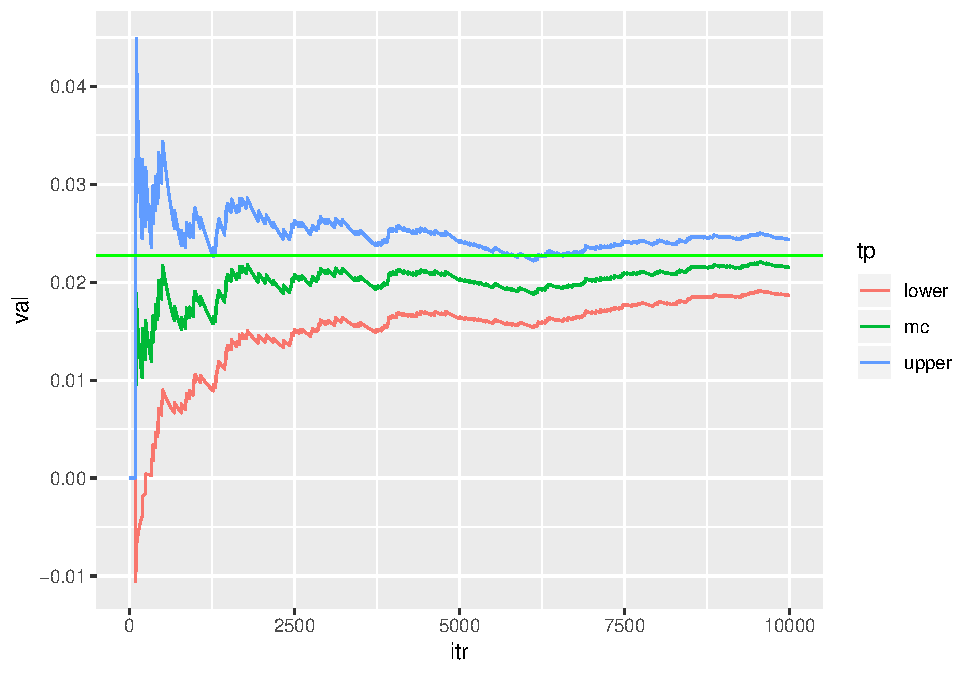
\includegraphics{bookdown-demo_files/figure-latex/unnamed-chunk-21-1.pdf}

\section{Importance sampling}\label{importance-sampling}

Importance sampling has samples generated from a different distribution
than the distribution of interest. Specifically, assume that we want to
calculate the expected value of \(h(x)\), and \(x \sim f(x)\).

\[E(h(x))=\int h(x) f(x) dx = \int h(x) \frac{f(x)}{g(x)} g(x) dx \] We
can sample \(x_i\) from \(g(x)\) and then calculate the mean of
\(h(x_i) \frac{f(x_i)}{g(x_i)}\).

Using the same explane above, we can use a shifted exponential
distribution to help calculate the intergral for normal distribution.
Specifically,

\[\int_2^{\infty} \frac{1}{2 \pi} e^{-\frac{1}{2}x^2}dx = \int_2^{\infty} \frac{\frac{1}{2 \pi} e^{-\frac{1}{2}x^2}}{e^{-(x-2)}} e^{-(x-2)}dx \]
The idea is that, we can generate \(x_i\) from exponential distribution
of \(e^{-(x-2)}\), and then insert them into the targeted ``expected
(value) function'' of
\(\frac{\frac{1}{2 \pi} e^{-\frac{1}{2}x^2}}{e^{-(x-2)}}\). Thus, as you
can see, importance sampling is based on the law of large numbers (i.e.,
If the same experiment or study is repeated independently a large number
of times, the average of the results of the trials must be close to the
expected value). We can use it to calculate integral based on link of
the definition of expected value.

\begin{Shaded}
\begin{Highlighting}[]
\NormalTok{Nsim=}\DecValTok{10}\OperatorTok{^}\DecValTok{4}
\NormalTok{normal_density=}\ControlFlowTok{function}\NormalTok{(x)}
\NormalTok{\{y=(}\DecValTok{1}\OperatorTok{/}\KeywordTok{sqrt}\NormalTok{(}\DecValTok{2}\OperatorTok{*}\NormalTok{pi))}\OperatorTok{*}\KeywordTok{exp}\NormalTok{(}\OperatorTok{-}\FloatTok{0.5}\OperatorTok{*}\NormalTok{(x}\OperatorTok{^}\DecValTok{2}\NormalTok{))}
\KeywordTok{return}\NormalTok{(y)\}}
\NormalTok{x=}\DecValTok{2}\OperatorTok{-}\KeywordTok{log}\NormalTok{(}\KeywordTok{runif}\NormalTok{(Nsim))}
\NormalTok{ImpS=}\KeywordTok{c}\NormalTok{(); v=}\KeywordTok{c}\NormalTok{(); upper=}\KeywordTok{c}\NormalTok{(); lower=}\KeywordTok{c}\NormalTok{()}
\ControlFlowTok{for}\NormalTok{ (j }\ControlFlowTok{in} \DecValTok{1}\OperatorTok{:}\NormalTok{Nsim)}
\NormalTok{\{}
\NormalTok{ImpS[j]=}\KeywordTok{mean}\NormalTok{(}\KeywordTok{normal_density}\NormalTok{(x[}\DecValTok{1}\OperatorTok{:}\NormalTok{j])}\OperatorTok{/}\KeywordTok{exp}\NormalTok{(}\OperatorTok{-}\NormalTok{(x[}\DecValTok{1}\OperatorTok{:}\NormalTok{j]}\OperatorTok{-}\DecValTok{2}\NormalTok{)))}
\NormalTok{v[j]=(j}\OperatorTok{^}\NormalTok{\{}\OperatorTok{-}\DecValTok{1}\NormalTok{\})}\OperatorTok{*}\KeywordTok{var}\NormalTok{(}\KeywordTok{normal_density}\NormalTok{(x[}\DecValTok{1}\OperatorTok{:}\NormalTok{j])}\OperatorTok{/}\KeywordTok{exp}\NormalTok{(}\OperatorTok{-}\NormalTok{(x[}\DecValTok{1}\OperatorTok{:}\NormalTok{j]}\OperatorTok{-}\DecValTok{2}\NormalTok{)))}
\NormalTok{upper[j]=ImpS[j]}\OperatorTok{+}\FloatTok{1.96}\OperatorTok{*}\KeywordTok{sqrt}\NormalTok{(v[j])}
\NormalTok{lower[j]=ImpS[j]}\OperatorTok{-}\FloatTok{1.96}\OperatorTok{*}\KeywordTok{sqrt}\NormalTok{(v[j])}
\NormalTok{\}}

\KeywordTok{library}\NormalTok{(ggplot2)}
\NormalTok{values=}\KeywordTok{c}\NormalTok{(ImpS,upper,lower)}
\NormalTok{type=}\KeywordTok{c}\NormalTok{(}\KeywordTok{rep}\NormalTok{(}\StringTok{"mc"}\NormalTok{,Nsim),}\KeywordTok{rep}\NormalTok{(}\StringTok{"upper"}\NormalTok{,Nsim),}\KeywordTok{rep}\NormalTok{(}\StringTok{"lower"}\NormalTok{,Nsim))}
\NormalTok{iter=}\KeywordTok{rep}\NormalTok{(}\KeywordTok{seq}\NormalTok{(}\DecValTok{1}\OperatorTok{:}\NormalTok{Nsim),}\DecValTok{3}\NormalTok{)}
\NormalTok{data=}\KeywordTok{data.frame}\NormalTok{(}\DataTypeTok{val=}\NormalTok{values, }\DataTypeTok{tp=}\NormalTok{type, }\DataTypeTok{itr=}\NormalTok{iter)}
\KeywordTok{ggplot}\NormalTok{(data,}\KeywordTok{aes}\NormalTok{(itr,val,}\DataTypeTok{col=}\NormalTok{tp))}\OperatorTok{+}\KeywordTok{geom_line}\NormalTok{(}\DataTypeTok{size=}\FloatTok{0.5}\NormalTok{)}\OperatorTok{+}
\KeywordTok{geom_hline}\NormalTok{(}\DataTypeTok{yintercept=}\DecValTok{1}\OperatorTok{-}\KeywordTok{pnorm}\NormalTok{(}\DecValTok{2}\NormalTok{),}\DataTypeTok{color=}\StringTok{"green"}\NormalTok{,}\DataTypeTok{size=}\FloatTok{0.5}\NormalTok{)}
\end{Highlighting}
\end{Shaded}

\begin{verbatim}
## Warning: Removed 2 rows containing missing values (geom_path).
\end{verbatim}

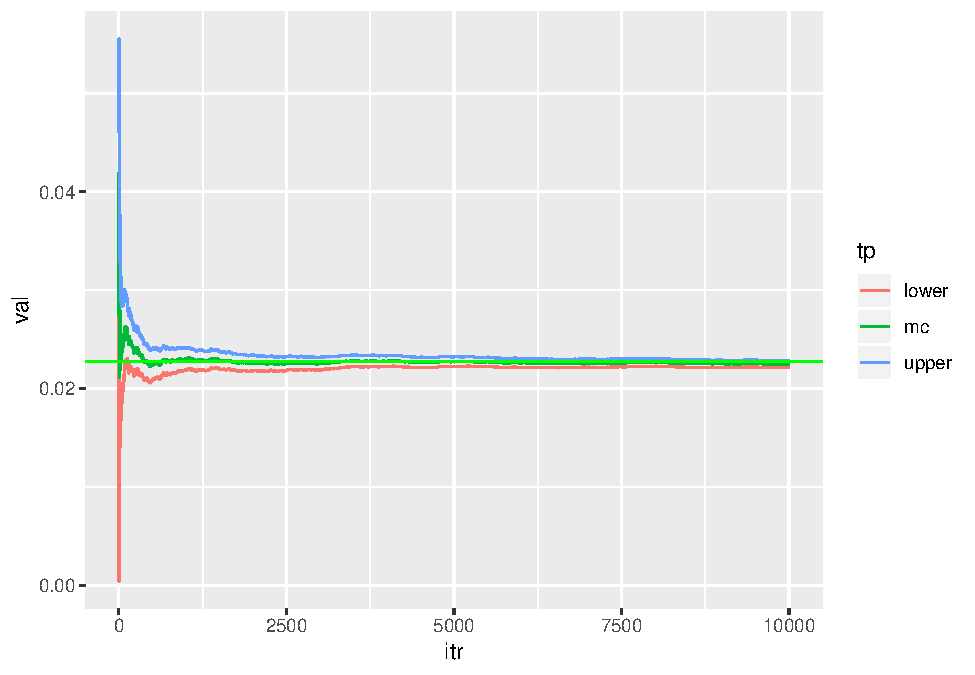
\includegraphics{bookdown-demo_files/figure-latex/unnamed-chunk-22-1.pdf}

\section{Newton Raphson algorithm}\label{newton-raphson-algorithm}

The main purpose of Newton Raphson algorithm is to calculate the root of
a function (e.g., \(x^2-3=0\)). We know that in order to maximize the
MLE, we need to calculate the first derivatice of the function and then
set it to zero \(\ell^{'}(x)=0\). Thus, we can use the same Newton
Raphson method to help calculate the MLE maximization as well.

There are different ways to understand Newton Raphson method, but I
found the method fo geometric the most easy way to explain.

\begin{figure}
\centering
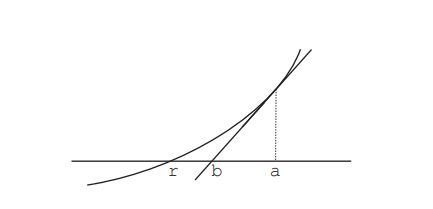
\includegraphics{Newton.jpg}
\caption{Credit of this figure:
\url{https://www.math.ubc.ca/~anstee/math104/newtonmethod.pdf}}
\end{figure}

Specifically, suppose that you want to calculate the root of a function
\(f(x)=0\). We assume the root is \(r\). However, we do not that, and we
randomly guess a point of \(a\). Thus, we can get a tangent line with
slope of \(f^{'}(a)\) and a point of \((a,f(a))\). Since we know the
slope and one of its points, we can write the function for this tangent
line.

\[y-f(a)=f^{'}(a)(x-a)\] To calculate the \(x-intercept\), namely \(b\)
in the figure, we can set \(y=0\), and get the following:

\[-f(a)=f^{'}(a)(x-a) \Rightarrow x (or, b)= a-\frac{f(a)}{f^{'}(a)}\]
If there is significant difference of \(|a-b|\), we know that our
orginal guess of \(a\) is not good. We better use \(b\) as the next
guess, and calculate its tangent line again. To generalize, we can write
it as follows. \[x_{t+1}=x_{t}-\frac{f(x_t)}{f^{'}(x_t)}\]

Okay, this method above is to calculate the root. For MLE, we can also
use this method to calculate the root for the \(\ell ^{'}=0\). We can
write it as follows.

\[x_{t+1}=x_{t}-\frac{\ell^{'}(x_t)}{\ell^{''}(x_t)}\] Often, \(x\) is
not just a single unknow parameter, but a vector. For this case, we can
write it as follows.

\[\beta_{t+1}=\beta_{t}-\frac{\ell^{'}(\beta_t)}{\ell^{''}(\beta_t)}\]

\subsection{Calculate the root}\label{calculate-the-root}

\(x^3-5=0\)

Note that, this is obviously not a maximization problem. In contrast, it
involves a function with zero. As we can see, we can think it as the
first order of Taylor approximation. That is, \(f^{'}(x)=x^3-5=0\). As
we can see the following plot, it converts very quickly.

\begin{Shaded}
\begin{Highlighting}[]
\NormalTok{f_firstorder=}\ControlFlowTok{function}\NormalTok{(x)\{x}\OperatorTok{^}\DecValTok{3}\OperatorTok{-}\DecValTok{5}\NormalTok{\}}
\NormalTok{f_secondorder=}\ControlFlowTok{function}\NormalTok{(x)\{}\DecValTok{3}\OperatorTok{*}\NormalTok{x\}}
\NormalTok{x_old=}\DecValTok{1}\NormalTok{;tolerance=}\FloatTok{1e-3}
\NormalTok{max_its=}\DecValTok{2000}\NormalTok{;iteration=}\DecValTok{1}\NormalTok{;difference=}\DecValTok{2}
\NormalTok{c_iteration<-}\KeywordTok{c}\NormalTok{() ## to collect numbers generated in the iteration process }
\ControlFlowTok{while}\NormalTok{(difference}\OperatorTok{>}\NormalTok{tolerance }\OperatorTok{&}\StringTok{ }\NormalTok{iteration}\OperatorTok{<}\NormalTok{max_its)\{}
\NormalTok{  x_updated=x_old}\OperatorTok{-}\NormalTok{(}\KeywordTok{f_firstorder}\NormalTok{(x_old)}\OperatorTok{/}\KeywordTok{f_secondorder}\NormalTok{(x_old))}
\NormalTok{  difference=}\KeywordTok{abs}\NormalTok{(x_updated}\OperatorTok{-}\NormalTok{x_old);}
\NormalTok{  iteration=iteration}\OperatorTok{+}\DecValTok{1}\NormalTok{;}
\NormalTok{  x_old=x_updated}
\NormalTok{  c_iteration<-}\KeywordTok{c}\NormalTok{(c_iteration,x_updated)\}}

\KeywordTok{plot}\NormalTok{(c_iteration,}\DataTypeTok{type=}\StringTok{"b"}\NormalTok{)}
\end{Highlighting}
\end{Shaded}

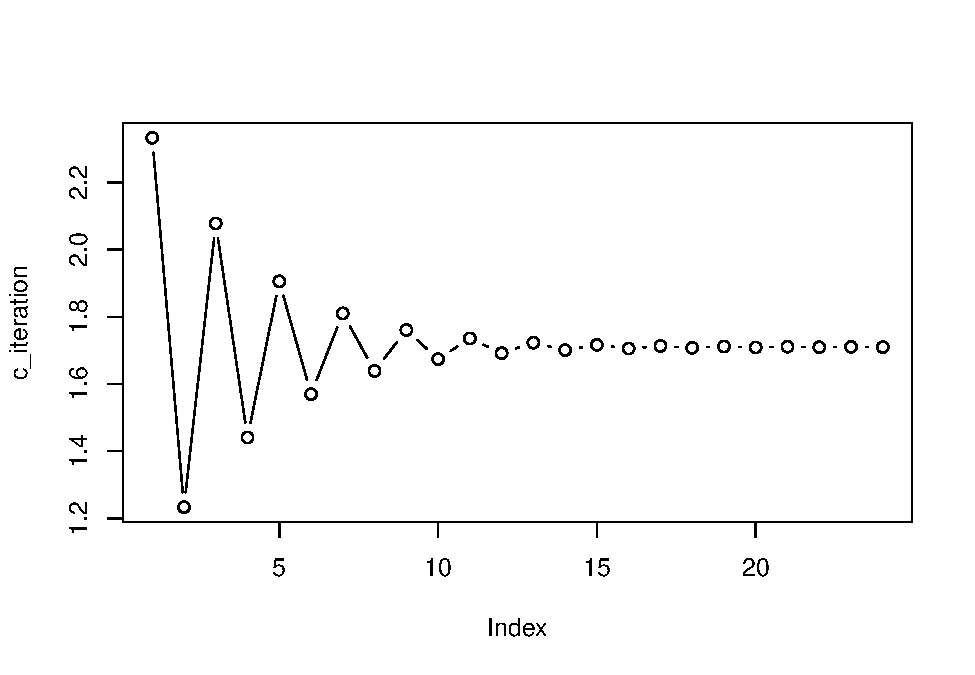
\includegraphics{bookdown-demo_files/figure-latex/unnamed-chunk-23-1.pdf}

\subsection{Logistic regression}\label{logistic-regression}

Suppose we have \(n\) observation, and \(m\) variables.

\[\begin{bmatrix}
x_{11} & x_{12} & x_{13} & ... & x_{1m}\\
x_{21} & x_{22} & x_{23} & ... & x_{2m} \\
...\\
x_{n1} & x_{n2} & x_{n3} & ... & x_{nm}
\end{bmatrix}\]

Typically, we add a vector of \(1\) being used to estimate the constant.

\[\begin{bmatrix}
1 & x_{11} & x_{12} & x_{13} & ... & x_{1m}\\
1 & x_{21} & x_{22} & x_{23} & ... & x_{2m} \\
...\\
1 & x_{n1} & x_{n2} & x_{n3} & ... & x_{nm}
\end{bmatrix}\]

And, we have observe a vector of \(n\) \(y_i\) as well, which is a
binary variable:

\[Y = \begin{bmatrix}1 \\
0 \\
1 \\
0 \\
0 \\
0 \\
...\\
1 \\
\end{bmatrix}\]

Using the content from the MLE chapter, we can get:

\[\mathbf{L}=\prod_{i=1}^{n} p_i^{ y_i}(1-p_i)^{(1-y_i)}\]

Further, we can get a log-transformed format.

\[log (\mathbf{L})=\sum_{i=1}^{n}[y_i log (p_i) + (1-y_i) log(1-p_i)]\]
Given that
\(p_i=\frac{e^{\beta_0+\beta_1x_1+...+\beta_nx_n}}{1+e^{\beta_0+\beta_1x_1+...+\beta_nx_n}}=\frac{e^{\beta^Tx}}{1+e^{\beta^Tx}}\),
we can rewrite it as follows:

\[log (\mathbf{L})=\ell=\sum_{i=1}^{n}[y_i log (\frac{e^{\beta^Tx_i}}{1+e^{\beta^Tx_i}}) + (1-y_i) log(1-\frac{e^{\beta^Tx_i}}{1+e^{\beta^Tx_i}})]\]
Before doing the derivative, we set.
\[\frac{e^{\beta^Tx_i}}{1+e^{\beta^Tx_i}} = p(\beta ^T x_i)\]

\[log (\mathbf{L})=\ell=\sum_{i=1}^{n}[y_i log (p(\beta ^T x_i)) + (1-y_i) log(1-p(\beta ^T x_i))]\]

Note that,
\(\frac{\partial p(\beta ^T x_i)}{\partial (\beta ^T x_i)} = p(\beta ^T x_i)(1-p(\beta ^T x_i))\).
We will use it later.

\[\begin{aligned}
\nabla \ell &= \sum_{i=1}^{n} [y_i \frac{1}{p(\beta ^T x_i)} \frac{\partial p(\beta ^T x_i)}{\partial (\beta ^T x_i)}\frac{\partial (\beta ^T x_i)}{\partial \beta}+(1-y_i) \frac{1}{1-p(\beta ^T x_i)}(-1)\frac{\partial p(\beta ^T x_i)}{\partial (\beta ^T x_i)}\frac{\partial (\beta ^T x_i)}{\partial \beta}] \\
&= \sum_{i=1}^{n} x_i^T[y_i \frac{1}{p(\beta ^T x_i)} p(\beta ^T x_i)(1-p(\beta ^T x_i))+(1-y_i) \frac{1}{1-p(\beta ^T x_i)}(-1)p(\beta ^T x_i)(1-p(\beta ^T x_i))] \\
&= \sum_{i=1}^{n} x_i^T[y_i \frac{1}{p(\beta ^T x_i)} p(\beta ^T x_i)(1-p(\beta ^T x_i))-(1-y_i) \frac{1}{1-p(\beta ^T x_i)}p(\beta ^T x_i)(1-p(\beta ^T x_i))] \\
&= \sum_{i=1}^{n} x_i^T[y_i (1-p(\beta ^T x_i))-(1-y_i) p(\beta ^T x_i)] \\
&=\sum_{i=1}^{n} x_i^T[y_i-y_ip(\beta ^T x_i)-p(\beta ^T x_i)+y_i p(\beta ^T x_i)] \\
&=\sum_{i=1}^{n} x_i^T[y_i-p(\beta ^T x_i)] \\
&= \sum_{i=1}^{n} x_i^T[y_i-\frac{e^{\beta^Tx_i}}{1+e^{\beta^Tx_i}}]
\end{aligned}\]

As noted, the Newton Raphson algorithm needs the second order.

\[\begin{aligned}
\nabla^2 \ell &=\frac{\partial \sum_{i=1}^{n} x_i^T[y_i-p(\beta ^T x_i)]}{\partial \beta} \\
&=-\sum_{i=1}^{n} x_i^T\frac{\partial p(\beta ^T x_i) }{\partial \beta}\\
&=-\sum_{i=1}^{n} x_i^T\frac{\partial p(\beta ^T x_i) }{\partial (\beta^Tx_i)} \frac{\partial (\beta^Tx_i)}{\partial \beta}\\
&=-\sum_{i=1}^{n} x_i^T p(\beta ^T x_i)(1-p(\beta ^T x_i))x_i
\end{aligned}\]

The following are the data simulation (3 IVs and 1 DV) and Newton
Raphson analysis.

\begin{Shaded}
\begin{Highlighting}[]
\CommentTok{# Data generation}
\KeywordTok{set.seed}\NormalTok{(}\DecValTok{123}\NormalTok{)}
\NormalTok{n=}\DecValTok{500}
\NormalTok{x1_norm<-}\KeywordTok{rnorm}\NormalTok{(n)}
\NormalTok{x2_norm<-}\KeywordTok{rnorm}\NormalTok{(n,}\DecValTok{3}\NormalTok{,}\DecValTok{4}\NormalTok{)}
\NormalTok{x3_norm<-}\KeywordTok{rnorm}\NormalTok{(n,}\DecValTok{4}\NormalTok{,}\DecValTok{6}\NormalTok{)}
\NormalTok{x_combined<-}\KeywordTok{cbind}\NormalTok{(}\DecValTok{1}\NormalTok{,x1_norm,x2_norm,x3_norm) }\CommentTok{# dimension: n*4}
\NormalTok{coefficients_new<-}\KeywordTok{c}\NormalTok{(}\DecValTok{1}\NormalTok{,}\DecValTok{2}\NormalTok{,}\DecValTok{3}\NormalTok{,}\DecValTok{4}\NormalTok{)  }\CommentTok{#true regression coefficient}
\NormalTok{inv_logit<-}\ControlFlowTok{function}\NormalTok{(x,b)\{}\KeywordTok{exp}\NormalTok{(x}\OperatorTok\NormalTok{b)}\OperatorTok{/}\NormalTok{(}\DecValTok{1}\OperatorTok{+}\KeywordTok{exp}\NormalTok{(x}\OperatorTok\NormalTok{b))\}}
\NormalTok{prob_generated<-}\KeywordTok{inv_logit}\NormalTok{(x_combined,coefficients_new)}
\NormalTok{y<-}\KeywordTok{c}\NormalTok{()}
\ControlFlowTok{for}\NormalTok{ (i }\ControlFlowTok{in} \DecValTok{1}\OperatorTok{:}\NormalTok{n) \{y[i]<-}\KeywordTok{rbinom}\NormalTok{(}\DecValTok{1}\NormalTok{,}\DecValTok{1}\NormalTok{,prob_generated[i])\}}

\CommentTok{# Newton Raphson}

\CommentTok{#We need to set random starting values.}
\NormalTok{beta_old<-}\KeywordTok{c}\NormalTok{(}\DecValTok{1}\NormalTok{,}\DecValTok{1}\NormalTok{,}\DecValTok{1}\NormalTok{,}\DecValTok{1}\NormalTok{)}
\NormalTok{tolerance=}\FloatTok{1e-3}
\NormalTok{max_its=}\DecValTok{2000}\NormalTok{;iteration=}\DecValTok{1}\NormalTok{;difference=}\DecValTok{2}
\NormalTok{W<-}\KeywordTok{matrix}\NormalTok{(}\DecValTok{0}\NormalTok{,n,n)}

\ControlFlowTok{while}\NormalTok{(difference}\OperatorTok{>}\NormalTok{tolerance }\OperatorTok{&}\StringTok{ }\NormalTok{iteration}\OperatorTok{<}\NormalTok{max_its)}
\NormalTok{  \{}
  \CommentTok{# The first order}
\NormalTok{  f_firstorder<-}\KeywordTok{t}\NormalTok{(x_combined)}\OperatorTok\NormalTok{(y}\OperatorTok{-}\KeywordTok{inv_logit}\NormalTok{(x_combined,beta_old))}
  \CommentTok{# The second order}
  \KeywordTok{diag}\NormalTok{(W) =}\StringTok{ }\KeywordTok{inv_logit}\NormalTok{(x_combined,beta_old)}\OperatorTok{*}\NormalTok{(}\DecValTok{1}\OperatorTok{-}\KeywordTok{inv_logit}\NormalTok{(x_combined,beta_old))}
\NormalTok{  f_secondorder<-}\OperatorTok{-}\KeywordTok{t}\NormalTok{(x_combined)}\OperatorTok\NormalTok{W}\OperatorTok\NormalTok{x_combined}
  \CommentTok{# Calculate the beta_updated}
\NormalTok{  beta_updated=beta_old}\OperatorTok{-}\NormalTok{(}\KeywordTok{solve}\NormalTok{(f_secondorder)}\OperatorTok\NormalTok{f_firstorder)}
\NormalTok{  difference=}\KeywordTok{max}\NormalTok{(}\KeywordTok{abs}\NormalTok{(beta_updated}\OperatorTok{-}\NormalTok{beta_old));}
\NormalTok{  iteration=iteration}\OperatorTok{+}\DecValTok{1}\NormalTok{;}
\NormalTok{  beta_old=beta_updated\}}

\NormalTok{beta_old}
\end{Highlighting}
\end{Shaded}

\begin{verbatim}
##              [,1]
##         0.9590207
## x1_norm 1.7974165
## x2_norm 3.0072303
## x3_norm 3.9578107
\end{verbatim}

\[\frac{\partial \ell} {\partial \beta} = \sum_{i=1}^{n} [y_i \frac{1}{p(\beta ^T x_i)} \frac{\partial p(\beta ^T x_i)}{\partial (\beta ^T x_i)}\frac{\partial (\beta ^T x_i)}{\partial \beta}+(1-y_i) \frac{1}{1-p(\beta ^T x_i)}(-1)\frac{\partial p(\beta ^T x_i)}{\partial (\beta ^T x_i)}\frac{\partial (\beta ^T x_i)}{\partial \beta}] \]
\[=\sum_{i=1}^{n} [y_i \frac{1}{p(\beta ^T x_i)} \phi (\beta ^T x_i)-(1-y_i) \frac{1}{1-p(\beta ^T x_i)}\phi (\beta ^T x_i)]x_i\]

\[\Phi(\beta_0+\beta_1x_1+\beta_2x_2+\beta_3x_3)= p(y=1)\]

\begin{Shaded}
\begin{Highlighting}[]
\CommentTok{# Data generation}
\NormalTok{n=}\DecValTok{500}
\NormalTok{x1_norm<-}\KeywordTok{rnorm}\NormalTok{(n)}
\NormalTok{x2_norm<-}\KeywordTok{rnorm}\NormalTok{(n)}
\NormalTok{x3_norm<-}\KeywordTok{rnorm}\NormalTok{(n)}
\NormalTok{x_combined<-}\KeywordTok{cbind}\NormalTok{(}\DecValTok{1}\NormalTok{,x1_norm,x2_norm,x3_norm)}
\NormalTok{coefficients_new<-}\KeywordTok{c}\NormalTok{(}\DecValTok{2}\NormalTok{,}\DecValTok{2}\NormalTok{,}\DecValTok{3}\NormalTok{,}\DecValTok{3}\NormalTok{)  }\CommentTok{#true regression coefficient}
\NormalTok{inv_norm<-}\ControlFlowTok{function}\NormalTok{(x,b)\{}\KeywordTok{pnorm}\NormalTok{(x}\OperatorTok\NormalTok{b)\}}
\NormalTok{prob_generated<-}\KeywordTok{inv_norm}\NormalTok{(x_combined,coefficients_new)}
\NormalTok{y<-}\KeywordTok{c}\NormalTok{()}
\ControlFlowTok{for}\NormalTok{ (i }\ControlFlowTok{in} \DecValTok{1}\OperatorTok{:}\NormalTok{n) \{y[i]<-}\KeywordTok{rbinom}\NormalTok{(}\DecValTok{1}\NormalTok{,}\DecValTok{1}\NormalTok{,prob_generated[i])\}}

\CommentTok{# Newton Raphson}

\CommentTok{#We need to set random starting values.}
\NormalTok{x_old<-}\KeywordTok{c}\NormalTok{(}\DecValTok{1}\NormalTok{,}\DecValTok{1}\NormalTok{,}\DecValTok{1}\NormalTok{,}\DecValTok{1}\NormalTok{)}
\NormalTok{tolerance=}\FloatTok{1e-3}
\NormalTok{max_its=}\DecValTok{2000}\NormalTok{;iteration=}\DecValTok{1}\NormalTok{;difference=}\DecValTok{2}

\ControlFlowTok{while}\NormalTok{(difference}\OperatorTok{>}\NormalTok{tolerance }\OperatorTok{&}\StringTok{ }\NormalTok{iteration}\OperatorTok{<}\NormalTok{max_its)\{}
\NormalTok{  x_updated=x_old}\OperatorTok{-}\NormalTok{(}\KeywordTok{f_firstorder}\NormalTok{(x_old)}\OperatorTok{/}\KeywordTok{f_secondorder}\NormalTok{(x_old))}
\NormalTok{  difference=}\KeywordTok{abs}\NormalTok{(x_updated}\OperatorTok{-}\NormalTok{x_old);}
\NormalTok{  iteration=iteration}\OperatorTok{+}\DecValTok{1}\NormalTok{;}
\NormalTok{  x_old=x_updated}
\NormalTok{  c_iteration<-}\KeywordTok{c}\NormalTok{(c_iteration,x_updated)\}}

\KeywordTok{plot}\NormalTok{(c_iteration,}\DataTypeTok{type=}\StringTok{"b"}\NormalTok{)}
\end{Highlighting}
\end{Shaded}

\section{Metropolis Hastings}\label{metropolis-hastings}

Metropolis--Hastings is a MCMC method for obtaining a sequence of random
samples from a probability distribution from which direct sampling is
difficult. By using the samples, we can plot the distribution (through
histgram), or we can calculate the integral (e.g., you need to calculate
the expected value).

(Side note: does this remind you the importance sampling? Very
similiar!)

Basic logic (my own summary):

\begin{enumerate}
\def\labelenumi{(\arabic{enumi})}
\item
  Set up a random starting value of \(x_0\).
\item
  Sample a \(y_0\) from the instrumental function of \(q(x)\).
\item
  Calculate the following:
\end{enumerate}

\(p =\frac{f(y_0)}{f(x_0)}\frac{q(x_0)}{q(y_0)}\)

\begin{enumerate}
\def\labelenumi{(\arabic{enumi})}
\setcounter{enumi}{3}
\item
  \(\rho=min(p, 1)\)
\item
  \(x_{1}=\begin{cases} y_0 & p \\ x_0 & 1-p \end{cases}\)
\item
  Repeat \(n\) times (\(n\) is set subjectively.)
\end{enumerate}

Use normal pdf to sample gamma distribution

\begin{Shaded}
\begin{Highlighting}[]
\NormalTok{alpha=}\FloatTok{2.7}\NormalTok{; beta=}\FloatTok{6.3} \CommentTok{# I randomly chose alpha and beta values for the target gamma function}

\NormalTok{Nsim=}\DecValTok{5000}\NormalTok{  ## define the number of iteration }

\NormalTok{X=}\KeywordTok{c}\NormalTok{(}\KeywordTok{rgamma}\NormalTok{(}\DecValTok{1}\NormalTok{,}\DecValTok{1}\NormalTok{)) }\CommentTok{# initialize the chain from random starting numbers}
\NormalTok{mygamma<-}\ControlFlowTok{function}\NormalTok{(Nsim,alpha,beta)\{}
\ControlFlowTok{for}\NormalTok{ (i }\ControlFlowTok{in} \DecValTok{2}\OperatorTok{:}\NormalTok{Nsim)\{}
\NormalTok{  Y=}\KeywordTok{rnorm}\NormalTok{(}\DecValTok{1}\NormalTok{)}
\NormalTok{  rho=}\KeywordTok{dgamma}\NormalTok{(Y,alpha,beta)}\OperatorTok{*}\KeywordTok{dnorm}\NormalTok{(X[i}\OperatorTok{-}\DecValTok{1}\NormalTok{])}\OperatorTok{/}\NormalTok{(}\KeywordTok{dgamma}\NormalTok{(X[i}\OperatorTok{-}\DecValTok{1}\NormalTok{],alpha,beta)}\OperatorTok{*}\KeywordTok{dnorm}\NormalTok{(Y))}
\NormalTok{  X[i]=X[i}\OperatorTok{-}\DecValTok{1}\NormalTok{] }\OperatorTok{+}\StringTok{ }\NormalTok{(Y}\OperatorTok{-}\NormalTok{X[i}\OperatorTok{-}\DecValTok{1}\NormalTok{])}\OperatorTok{*}\NormalTok{(}\KeywordTok{runif}\NormalTok{(}\DecValTok{1}\NormalTok{)}\OperatorTok{<}\NormalTok{rho)}
\NormalTok{\}}
\NormalTok{X}
\NormalTok{\}}

\KeywordTok{hist}\NormalTok{(}\KeywordTok{mygamma}\NormalTok{(Nsim,alpha,beta), }\DataTypeTok{breaks =} \DecValTok{100}\NormalTok{)}
\end{Highlighting}
\end{Shaded}

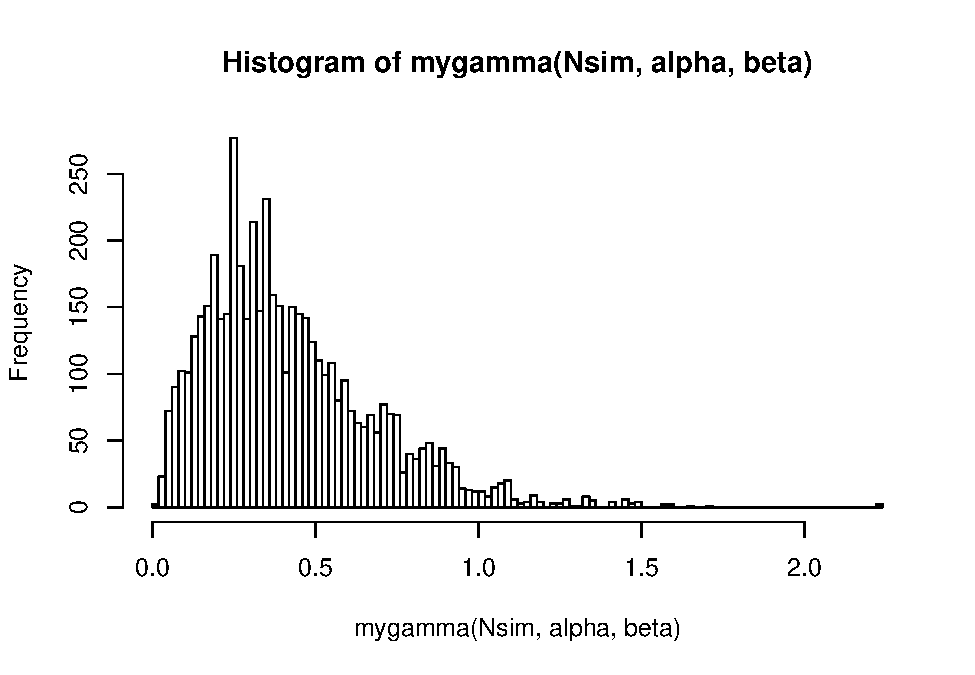
\includegraphics{bookdown-demo_files/figure-latex/unnamed-chunk-26-1.pdf}

\section{EM}\label{em}

EM algorithm is an iterative method to find ML or maximum a posteriori
(MAP) estimates of parameters.

Direct Ref: \url{http://www.di.fc.ul.pt/~jpn/r/EM/EM.html}

Suppose that we only observe \(X\), and do not know \(Z\). We thus need
to construct the complete data of \((X, Z)\). Given \(p(Z|X,\theta)\),
we can compute the likelihood of the complete dataset:

\[p(X, Z|\theta)=p(Z|X,\theta)p(X|\theta)\] The EM algorithm:

\begin{enumerate}
\def\labelenumi{(\arabic{enumi})}
\setcounter{enumi}{-1}
\item
  We got \(X\) and \(p(Z|X,\theta)\)
\item
  Random assign a \(\theta_0\), since we do not know any of them.
\item
  E-step: \(Q_{\theta_i} = E_{Z|X,\theta_i}[log p(X,Z|\theta)]\)
\item
  M-step: compute \(\theta_{i+1} \leftarrow argmax Q_{\theta_i}\)
\item
  If \(\theta_i\) and \(\theta_{i+1}\) are not close enough,
  \(\theta_i \leftarrow \theta_{i+1}\). Goto step 2.
\end{enumerate}

For examples, you can refer to the following link:
\url{http://www.di.fc.ul.pt/~jpn/r/EM/EM.html}

(It is em\_R.r in R\_codes folder. Personally, I can also refer to Quiz
2 in 536.)

\section{References}\label{references-2}

\begin{enumerate}
\def\labelenumi{\arabic{enumi}.}
\tightlist
\item
  The UBC PDF about Newton
\end{enumerate}

\url{https://www.math.ubc.ca/~anstee/math104/newtonmethod.pdf}

\begin{enumerate}
\def\labelenumi{\arabic{enumi}.}
\setcounter{enumi}{1}
\tightlist
\item
  Some other pages about Newton and logistic regression
\end{enumerate}

\url{http://www.win-vector.com/blog/2011/09/the-simpler-derivation-of-logistic-regression/}

\url{https://stats.stackexchange.com/questions/344309/why-using-newtons-method-for-logistic-regression-optimization-is-called-iterati}

\url{https://tomroth.com.au/logistic/}

\url{https://www.stat.cmu.edu/~cshalizi/350/lectures/26/lecture-26.pdf}

\url{https://www.stat.cmu.edu/~cshalizi/402/lectures/14-logistic-regression/lecture-14.pdf}

\url{http://hua-zhou.github.io/teaching/biostatm280-2017spring/slides/18-newton/newton.html}

\begin{enumerate}
\def\labelenumi{\arabic{enumi}.}
\setcounter{enumi}{2}
\tightlist
\item
  MH
\end{enumerate}

\url{https://www.youtube.com/watch?v=VGRVRjr0vyw}

\chapter{Generalized Linear Mixed
Models}\label{generalized-linear-mixed-models}

\section{Basics of GLMM}\label{basics-of-glmm}

Recall the formula in the probit model:

\[Y^*=X\beta+\epsilon, \epsilon \sim N(0,\sigma^2)=N(0,I)\] Similar to
LMM, binary model with random effect can be written as follows.

\[Y^*=X\beta+ Z u+\epsilon\] where,

\[\epsilon \sim N(0,I)\] \[u \sim N(0, D)\]

We also assume \(\epsilon\) and \(u\) are independent.Thus, we know that
\(D\) represents the virances of the random effects. If we make
\(u =1\), the model becomes the usual probit model. McCulloch (1994)
states that there are a few advantages to use probit, rather than logit
models. (Note that, however, probit is not canonical link function, but
logit is!)

The following is the note from Charle E. McCulloch's ``Maximum
likelihood algorithems for Generalized Linear Mixed Models''

\section{Some References}\label{some-references}

\url{http://www.biostat.umn.edu/~baolin/teaching/linmods/glmm.html}

\url{http://www.biostat.umn.edu/~baolin/teaching/probmods/GLMM_mcmc.html}

\url{https://bbolker.github.io/mixedmodels-misc/glmmFAQ.html}

\chapter{Twitter Example}\label{twitter-example}

The following is part of my course project for Stat 536. It aims to
replicate part of the findings from Barbera (2015) Birds of the Same
Feather Tweet Together: Bayesian Ideal Point Estimation Using Twitter
Data. Political Analysis 23 (1). Note that, the following model is much
simpler than that in the original paper.

\section{Model}\label{model}

Suppose that a Twitter user is presented with a choice between following
or not following another target \(j \in \{ 1, ..., m\}\). Let
\(y_{j}=1\) if the user decides to follow \(j\), and \(y_{j}=0\)
otherwise.

\[y_{j}=\begin{cases} 1 & Following \\ 0 & Not Following \end{cases}\]

\[p(y_{j}=1|\theta) = \frac{exp(- \theta_0|\theta_1 - x_j|^2)}{1+exp(- \theta_0|\theta_1 - x_j|^2)}\]
We additionally know the priors of \(\theta\).

\[\theta_i \sim N(0,10^2) (i = 0, 1)\]

The likelihood function is as follows.

\[L(Y|\theta)=\prod_{j=1}^{m} (\frac{exp(- \theta_0|\theta_1 - x_j|^2)}{1+exp(- \theta_0|\theta_1 - x_j|^2)})^{y_j}(1-\frac{exp(- \theta_0|\theta_1 - x_j|^2)}{1+exp(- \theta_0|\theta_1 - x_j|^2)})^{(1-y_j)}\]
Thus, the posterior is as follows.

\[L(Y|\theta) \cdot N(\theta_0|0,10) \cdot N(\theta_1|0,10)\]
\[\propto \prod_{j=1}^{m} (\frac{exp(- \theta_0|\theta_1 - x_j|^2)}{1+exp(- \theta_0|\theta_1 - x_j|^2)})^{y_j}(1-\frac{exp(- \theta_0|\theta_1 - x_j|^2)}{1+exp(- \theta_0|\theta_1 - x_j|^2)})^{(1-y_j)}\cdot exp(-\frac{1}{2}(\frac{\theta_0}{10})^2)\cdot exp(-\frac{1}{2}(\frac{\theta_1}{10})^2)\]

\begin{Shaded}
\begin{Highlighting}[]
\CommentTok{#Establish the function for logistic regression}
\NormalTok{Expit<-}\ControlFlowTok{function}\NormalTok{(x)\{}\KeywordTok{exp}\NormalTok{(x)}\OperatorTok{/}\NormalTok{(}\DecValTok{1}\OperatorTok{+}\KeywordTok{exp}\NormalTok{(x))\}}

\CommentTok{#Construct the posterior - in a log-format}
\CommentTok{#To make sure that the estimate of theta_1 is stable, }
\CommentTok{#the following code wants to make sure that theta_0 is always greater than zero.}

\NormalTok{log_post<-}\ControlFlowTok{function}\NormalTok{(Y, X, theta)}
\NormalTok{  \{}
  \ControlFlowTok{if}\NormalTok{(theta[}\DecValTok{1}\NormalTok{]}\OperatorTok{<=}\DecValTok{0}\NormalTok{)\{post=}\OperatorTok{-}\OtherTok{Inf}\NormalTok{\}}
  \ControlFlowTok{if}\NormalTok{(theta[}\DecValTok{1}\NormalTok{]}\OperatorTok{>}\DecValTok{0}\NormalTok{)\{}
\NormalTok{  prob1<-}\KeywordTok{Expit}\NormalTok{(}\OperatorTok{-}\NormalTok{theta[}\DecValTok{1}\NormalTok{]}\OperatorTok{*}\NormalTok{((theta[}\DecValTok{2}\NormalTok{]}\OperatorTok{-}\NormalTok{X)}\OperatorTok{^}\DecValTok{2}\NormalTok{))}
\NormalTok{  likelihood<-}\KeywordTok{sum}\NormalTok{(}\KeywordTok{dbinom}\NormalTok{(Y,}\DecValTok{1}\NormalTok{,prob1,}\DataTypeTok{log =} \OtherTok{TRUE}\NormalTok{))}
\NormalTok{  priors<-}\KeywordTok{sum}\NormalTok{(}\KeywordTok{dnorm}\NormalTok{(theta,}\DecValTok{0}\NormalTok{,}\DecValTok{10}\NormalTok{,}\DataTypeTok{log=}\OtherTok{TRUE}\NormalTok{))}
\NormalTok{  post=likelihood}\OperatorTok{+}\NormalTok{priors\}}
  \KeywordTok{return}\NormalTok{(post)}
\NormalTok{   \}}

\NormalTok{Bayes_logit<-}\ControlFlowTok{function}\NormalTok{ (Y,X,}\DataTypeTok{n_samples=}\DecValTok{2000}\NormalTok{)}
\NormalTok{\{}
\CommentTok{#Initial values}
\NormalTok{  theta<-}\KeywordTok{c}\NormalTok{(}\DecValTok{5}\NormalTok{,}\DecValTok{5}\NormalTok{)}
\CommentTok{#store data}
\NormalTok{  keep.theta<-}\KeywordTok{matrix}\NormalTok{(}\DecValTok{0}\NormalTok{,n_samples,}\DecValTok{2}\NormalTok{)}
\NormalTok{  keep.theta[}\DecValTok{1}\NormalTok{,]<-theta}
  
\CommentTok{#acceptance and rejection  }
\NormalTok{  acc<-att<-}\KeywordTok{rep}\NormalTok{(}\DecValTok{0}\NormalTok{,}\DecValTok{2}\NormalTok{)}
\CommentTok{#current log posterior}
\NormalTok{  current_lp<-}\KeywordTok{log_post}\NormalTok{(Y,X,theta)}

  \ControlFlowTok{for}\NormalTok{ (i }\ControlFlowTok{in} \DecValTok{2}\OperatorTok{:}\NormalTok{n_samples)  }
\NormalTok{  \{}
    
    \ControlFlowTok{for}\NormalTok{(j }\ControlFlowTok{in} \DecValTok{1}\OperatorTok{:}\DecValTok{2}\NormalTok{)}
\NormalTok{    \{}
      \CommentTok{#attempt + 1}
\NormalTok{      att[j]<-att[j]}\OperatorTok{+}\DecValTok{1}
\NormalTok{      can_theta<-theta}
\NormalTok{      can_theta[j]<-}\KeywordTok{rnorm}\NormalTok{(}\DecValTok{1}\NormalTok{,theta[j],}\FloatTok{0.5}\NormalTok{)}
      \CommentTok{#candidate of log posterior}
\NormalTok{      candidate_lp<-}\KeywordTok{log_post}\NormalTok{(Y,X,can_theta)}
\NormalTok{      Rho<-}\KeywordTok{min}\NormalTok{(}\KeywordTok{exp}\NormalTok{(candidate_lp}\OperatorTok{-}\NormalTok{current_lp),}\DecValTok{1}\NormalTok{)}
\NormalTok{      Random_probability<-}\KeywordTok{runif}\NormalTok{(}\DecValTok{1}\NormalTok{)}
      \ControlFlowTok{if}\NormalTok{ (Random_probability}\OperatorTok{<}\NormalTok{Rho)}
\NormalTok{      \{}
\NormalTok{        theta<-can_theta}
\NormalTok{        current_lp<-candidate_lp}
        \CommentTok{#acceptance + 1, as long as Random_probability<Rho}
\NormalTok{        acc[j]<-acc[j]}\OperatorTok{+}\DecValTok{1}
\NormalTok{      \}}
\NormalTok{    \}}
    \CommentTok{#save theta}
\NormalTok{    keep.theta[i,]<-theta}
\NormalTok{  \}}
\CommentTok{#Return: including theta and acceptance rate}
  \KeywordTok{list}\NormalTok{(}\DataTypeTok{theta=}\NormalTok{keep.theta,}\DataTypeTok{acceptance_rate=}\NormalTok{acc}\OperatorTok{/}\NormalTok{att)}
\NormalTok{\}}
\end{Highlighting}
\end{Shaded}

\section{Simulating Data of Senators on
Twitter}\label{simulating-data-of-senators-on-twitter}

Assume that we have 100 senators, 50 Democrats and 50 Republicans, who
we know their ideology. Assume that Democrats have negative ideology
scores to indicate that they are more liberal, whereas Republicans have
positive scores to indicate that they are more conservative. The
following is data simulation for senators.

\begin{Shaded}
\begin{Highlighting}[]
\CommentTok{# Republicans are more conservative, and they have positive numbers.}
\NormalTok{Republicans<-}\KeywordTok{c}\NormalTok{()}
\NormalTok{Republicans<-}\KeywordTok{rnorm}\NormalTok{(}\DecValTok{50}\NormalTok{,}\DecValTok{1}\NormalTok{,}\FloatTok{0.5}\NormalTok{)}
\NormalTok{No_Republicans<-}\KeywordTok{rep}\NormalTok{(}\DecValTok{1}\OperatorTok{:}\DecValTok{50}\NormalTok{,}\DecValTok{1}\NormalTok{)}
\NormalTok{Part_}\DecValTok{1}\NormalTok{<-}\KeywordTok{cbind}\NormalTok{(No_Republicans,Republicans)}

\CommentTok{# Democrats are more liberal, and they have negative numbers.}
\NormalTok{Democrats<-}\KeywordTok{c}\NormalTok{()}
\NormalTok{Democrats<-}\KeywordTok{rnorm}\NormalTok{(}\DecValTok{50}\NormalTok{,}\OperatorTok{-}\DecValTok{1}\NormalTok{,}\FloatTok{0.5}\NormalTok{)}
\NormalTok{No_Democrats<-}\KeywordTok{rep}\NormalTok{(}\DecValTok{51}\OperatorTok{:}\DecValTok{100}\NormalTok{,}\DecValTok{1}\NormalTok{)}
\NormalTok{Part_}\DecValTok{2}\NormalTok{<-}\KeywordTok{cbind}\NormalTok{(No_Democrats,Democrats)}
\NormalTok{Data_Elites<-}\KeywordTok{rbind}\NormalTok{(Part_}\DecValTok{1}\NormalTok{,Part_}\DecValTok{2}\NormalTok{)}
\NormalTok{Data_Elites<-}\KeywordTok{as.data.frame}\NormalTok{(Data_Elites)}
\KeywordTok{colnames}\NormalTok{(Data_Elites) <-}\StringTok{ }\KeywordTok{c}\NormalTok{(}\StringTok{"Elite_No"}\NormalTok{,}\StringTok{"Elite_ideology"}\NormalTok{)}

\KeywordTok{head}\NormalTok{(Data_Elites)}
\end{Highlighting}
\end{Shaded}

\begin{verbatim}
##   Elite_No Elite_ideology
## 1        1      1.0541992
## 2        2      0.3805544
## 3        3      1.3568577
## 4        4      0.9922547
## 5        5      1.0089966
## 6        6      0.8878271
\end{verbatim}

\section{Simulating Data of Conservative Users on Twitter and Model
Testing}\label{simulating-data-of-conservative-users-on-twitter-and-model-testing}

Assume that we observe one Twitter user, who is more conservative. To
simulate Twitter following data for this user, I assign this user to
follow more Republican senators. Thus, if the Metropolis Hastings
algorithm works as intended, we would expect to see a positive estimated
value for their ideology. Importantly, as we can see in the histogram
below, the estimated value indeed is positive, providing preliminary
evidence for the statistical model and the algorithm. In addition, for
the acceptance rate, we can see that the constant has a lower number
than ideology, since we only accept a constant when it is positive.

\begin{Shaded}
\begin{Highlighting}[]
\CommentTok{#This user approximately follows 45 Republican Senators and 10 Democrat Senators. }
\NormalTok{Data_user<-}\KeywordTok{as.data.frame}\NormalTok{(}\KeywordTok{matrix}\NormalTok{(}\KeywordTok{c}\NormalTok{(}\KeywordTok{ifelse}\NormalTok{(}\KeywordTok{runif}\NormalTok{(}\DecValTok{50}\NormalTok{)}\OperatorTok{<}\NormalTok{.}\DecValTok{1}\NormalTok{,}\DecValTok{0}\NormalTok{,}\DecValTok{1}\NormalTok{),}\KeywordTok{ifelse}\NormalTok{(}\KeywordTok{runif}\NormalTok{(}\DecValTok{50}\NormalTok{)}\OperatorTok{<}\NormalTok{.}\DecValTok{8}\NormalTok{,}\DecValTok{0}\NormalTok{,}\DecValTok{1}\NormalTok{))), }\DecValTok{100}\NormalTok{, }\DecValTok{1}\NormalTok{)}
\KeywordTok{colnames}\NormalTok{(Data_user)<-}\KeywordTok{c}\NormalTok{(}\StringTok{"R_User"}\NormalTok{)}
\NormalTok{Data_combined<-}\KeywordTok{cbind}\NormalTok{(Data_Elites,Data_user)}

\NormalTok{X_data<-Data_combined}\OperatorTok{$}\NormalTok{Elite_ideology}
\NormalTok{Y_data<-Data_combined}\OperatorTok{$}\NormalTok{R_User}

\NormalTok{fit_C<-}\KeywordTok{Bayes_logit}\NormalTok{(Y_data,X_data)}
\NormalTok{fit_C}\OperatorTok{$}\NormalTok{acceptance_rate}
\end{Highlighting}
\end{Shaded}

\begin{verbatim}
## [1] 0.1320660 0.5557779
\end{verbatim}

\begin{Shaded}
\begin{Highlighting}[]
\KeywordTok{plot}\NormalTok{(fit_C}\OperatorTok{$}\NormalTok{theta[,}\DecValTok{1}\NormalTok{],}\DataTypeTok{main=}\StringTok{"Constant (Conservative Users)"}\NormalTok{,}
     \DataTypeTok{xlab=}\StringTok{"Iteration Process"}\NormalTok{,}\DataTypeTok{ylab=}\StringTok{"Estimated Scores"}\NormalTok{,}\DataTypeTok{type=}\StringTok{"l"}\NormalTok{)}
\end{Highlighting}
\end{Shaded}

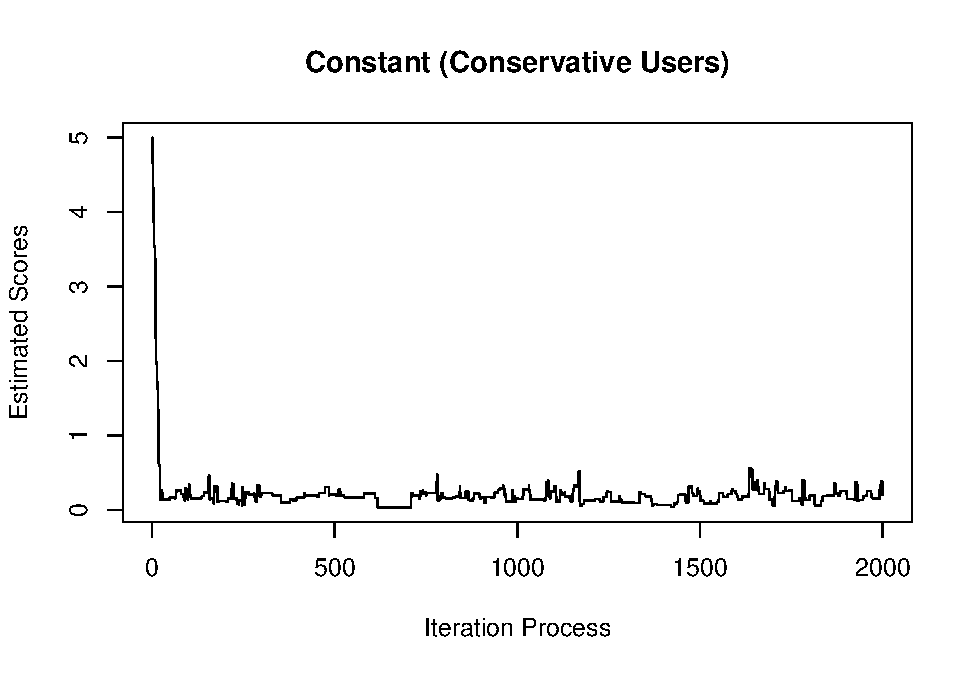
\includegraphics{bookdown-demo_files/figure-latex/unnamed-chunk-29-1.pdf}

\begin{Shaded}
\begin{Highlighting}[]
\KeywordTok{plot}\NormalTok{(fit_C}\OperatorTok{$}\NormalTok{theta[,}\DecValTok{2}\NormalTok{],}\DataTypeTok{main=}\StringTok{"Estimated Ideology Scores (Conservative Users)"}\NormalTok{,}
     \DataTypeTok{xlab=}\StringTok{"Iteration Process"}\NormalTok{,}\DataTypeTok{ylab=}\StringTok{"Ideology Scores"}\NormalTok{,}\DataTypeTok{type=}\StringTok{"l"}\NormalTok{)}
\end{Highlighting}
\end{Shaded}

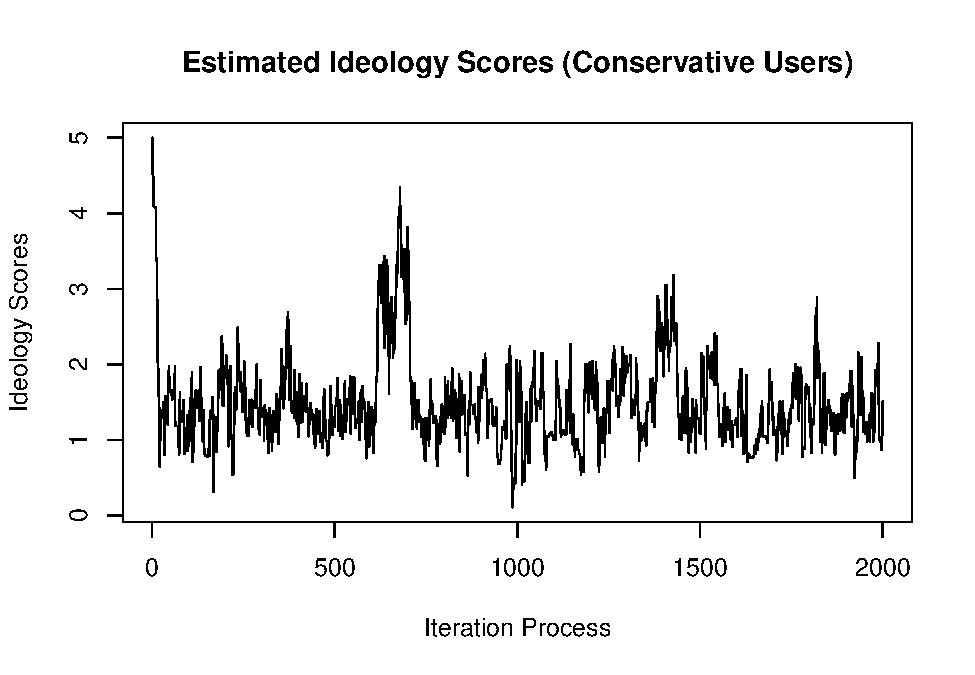
\includegraphics{bookdown-demo_files/figure-latex/unnamed-chunk-29-2.pdf}

\begin{Shaded}
\begin{Highlighting}[]
\KeywordTok{hist}\NormalTok{(fit_C}\OperatorTok{$}\NormalTok{theta[,}\DecValTok{2}\NormalTok{],}\DataTypeTok{main=}\StringTok{"Estimated Ideology Scores (Conservative Users)"}\NormalTok{,}
     \DataTypeTok{xlab=}\StringTok{"Ideology Scores"}\NormalTok{,}\DataTypeTok{breaks =} \DecValTok{100}\NormalTok{)}
\end{Highlighting}
\end{Shaded}

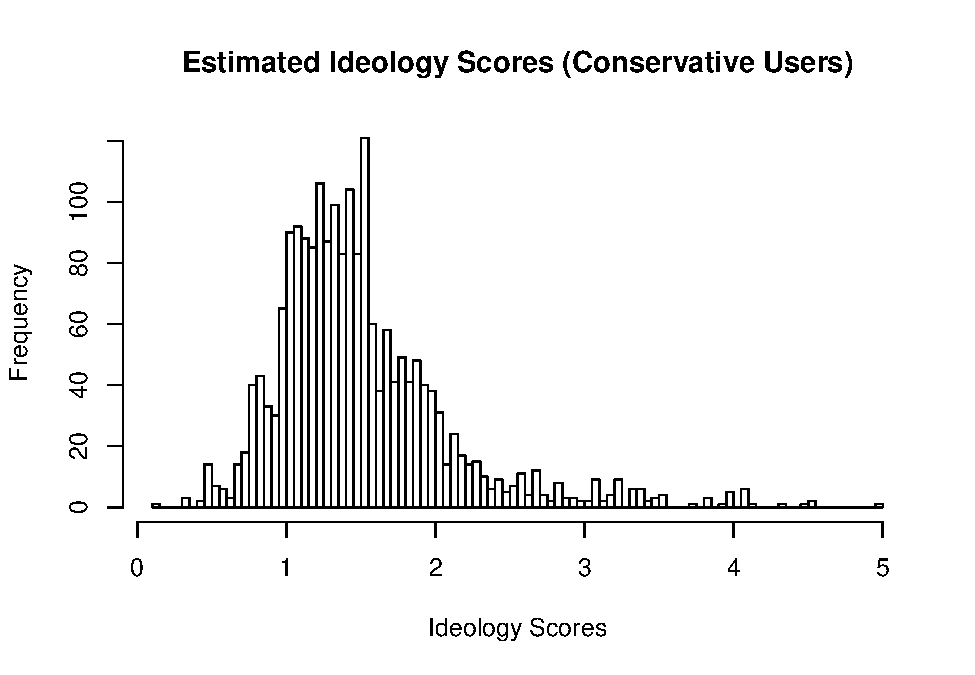
\includegraphics{bookdown-demo_files/figure-latex/unnamed-chunk-29-3.pdf}

\section{Simulating Data of Liberal Users on Twitter and Model
Testing}\label{simulating-data-of-liberal-users-on-twitter-and-model-testing}

To further verify the Metropolis Hastings algorithm, I plan to test the
opposite estimate. Specifically, assume that we observe another user,
who is more liberal. To simulate Twitter following data for this user, I
assign this user to follow more Democrat senators. In this case, we
would expect to see a negative value for their estimated ideology. As we
can see in the histogram shown below, as expected, the estimated value
is negative, providing convergent evidence for the model and the
algorithm.

\begin{Shaded}
\begin{Highlighting}[]
\CommentTok{#This user approximately follows 10 Republican Senators and 45 Democrat Senators. }
\NormalTok{Data_user<-}\KeywordTok{as.data.frame}\NormalTok{(}\KeywordTok{matrix}\NormalTok{(}\KeywordTok{c}\NormalTok{(}\KeywordTok{ifelse}\NormalTok{(}\KeywordTok{runif}\NormalTok{(}\DecValTok{50}\NormalTok{)}\OperatorTok{<}\NormalTok{.}\DecValTok{8}\NormalTok{,}\DecValTok{0}\NormalTok{,}\DecValTok{1}\NormalTok{),}\KeywordTok{ifelse}\NormalTok{(}\KeywordTok{runif}\NormalTok{(}\DecValTok{50}\NormalTok{)}\OperatorTok{<}\NormalTok{.}\DecValTok{1}\NormalTok{,}\DecValTok{0}\NormalTok{,}\DecValTok{1}\NormalTok{))), }\DecValTok{100}\NormalTok{, }\DecValTok{1}\NormalTok{)}
\KeywordTok{colnames}\NormalTok{(Data_user)<-}\KeywordTok{c}\NormalTok{(}\StringTok{"L_User"}\NormalTok{)}
\NormalTok{Data_combined<-}\KeywordTok{cbind}\NormalTok{(Data_Elites,Data_user)}

\NormalTok{X_data<-Data_combined}\OperatorTok{$}\NormalTok{Elite_ideology}
\NormalTok{Y_data<-Data_combined}\OperatorTok{$}\NormalTok{L_User}


\NormalTok{fit_L<-}\KeywordTok{Bayes_logit}\NormalTok{(Y_data,X_data)}
\NormalTok{fit_L}\OperatorTok{$}\NormalTok{acceptance_rate}
\end{Highlighting}
\end{Shaded}

\begin{verbatim}
## [1] 0.1585793 0.5092546
\end{verbatim}

\begin{Shaded}
\begin{Highlighting}[]
\KeywordTok{plot}\NormalTok{(fit_L}\OperatorTok{$}\NormalTok{theta[,}\DecValTok{1}\NormalTok{],}\DataTypeTok{main=}\StringTok{"Constant (Liberal Users)"}\NormalTok{,}
     \DataTypeTok{xlab=}\StringTok{"Iteration Process"}\NormalTok{,}\DataTypeTok{ylab=}\StringTok{"Estimated Scores"}\NormalTok{,}\DataTypeTok{type=}\StringTok{"l"}\NormalTok{)}
\end{Highlighting}
\end{Shaded}

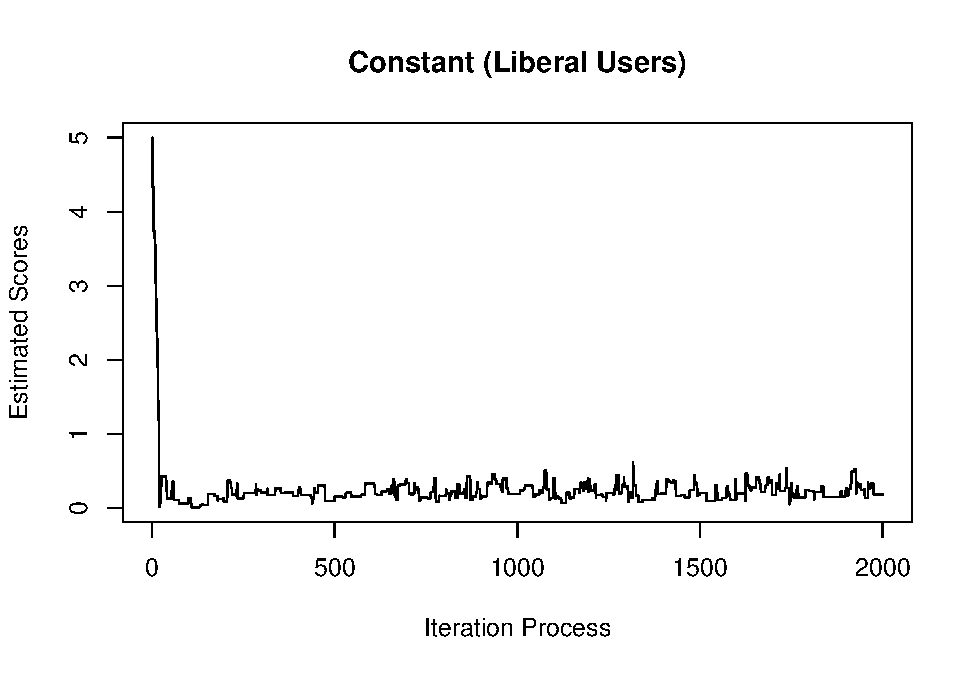
\includegraphics{bookdown-demo_files/figure-latex/unnamed-chunk-30-1.pdf}

\begin{Shaded}
\begin{Highlighting}[]
\KeywordTok{plot}\NormalTok{(fit_L}\OperatorTok{$}\NormalTok{theta[,}\DecValTok{2}\NormalTok{],}\DataTypeTok{main=}\StringTok{"Estimated Ideology Scores (Liberal Users)"}\NormalTok{,}
     \DataTypeTok{xlab=}\StringTok{"Iteration Process"}\NormalTok{,}\DataTypeTok{ylab=}\StringTok{"Ideology Scores"}\NormalTok{,}\DataTypeTok{type=}\StringTok{"l"}\NormalTok{)}
\end{Highlighting}
\end{Shaded}

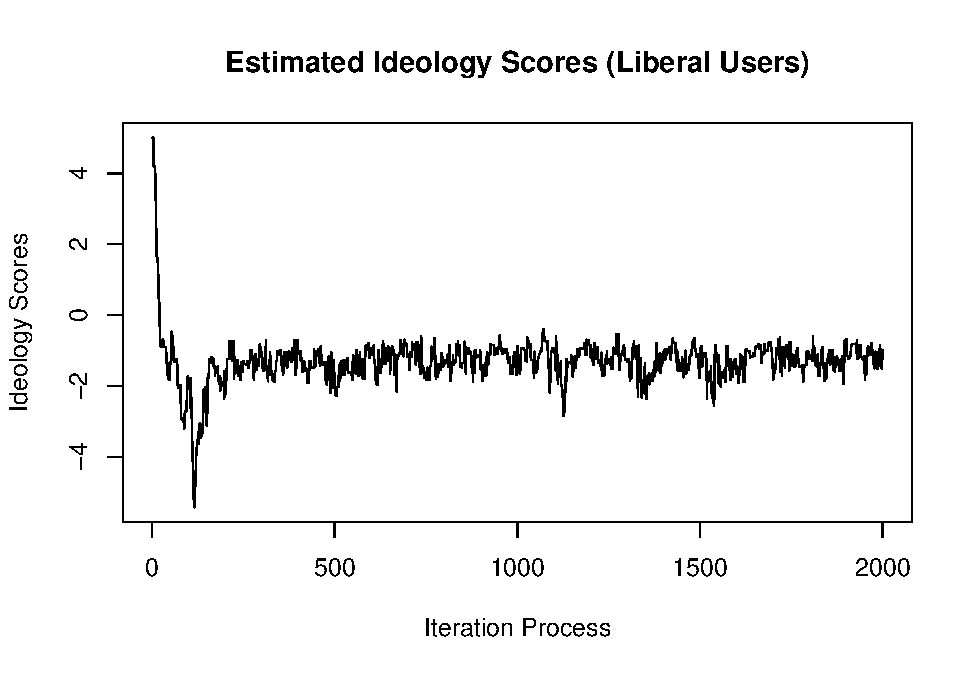
\includegraphics{bookdown-demo_files/figure-latex/unnamed-chunk-30-2.pdf}

\begin{Shaded}
\begin{Highlighting}[]
\KeywordTok{hist}\NormalTok{(fit_L}\OperatorTok{$}\NormalTok{theta[,}\DecValTok{2}\NormalTok{],}\DataTypeTok{main=}\StringTok{"Estimated Ideology Scores (Liberal Users)"}\NormalTok{,}
     \DataTypeTok{xlab=}\StringTok{"Ideology Scores"}\NormalTok{,}\DataTypeTok{breaks =} \DecValTok{100}\NormalTok{)}
\end{Highlighting}
\end{Shaded}

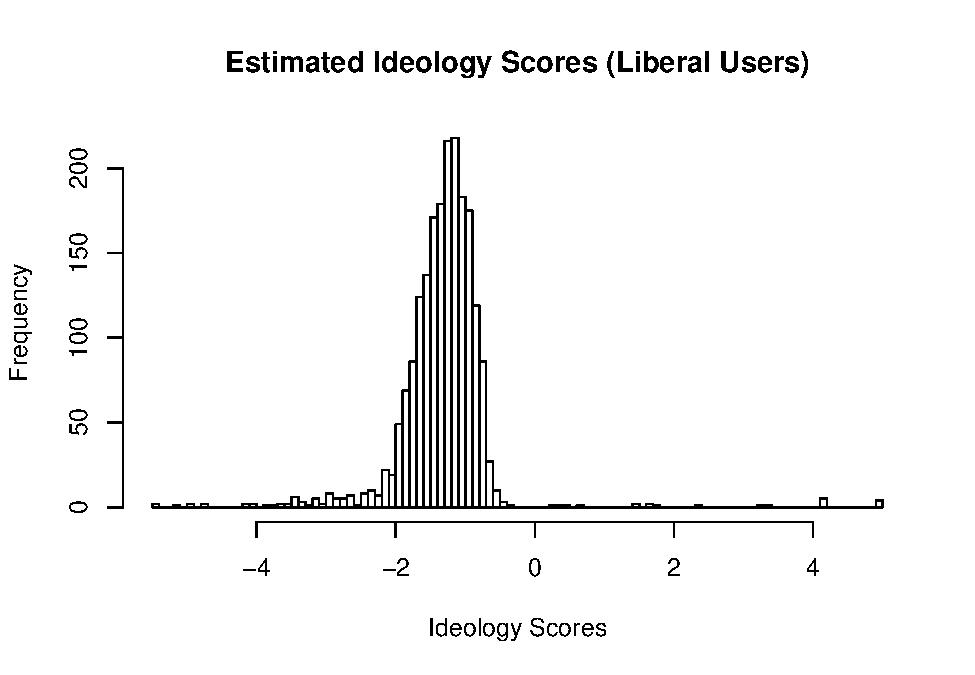
\includegraphics{bookdown-demo_files/figure-latex/unnamed-chunk-30-3.pdf}

\chapter{Practice: Learning on the Battle
Field}\label{practice-learning-on-the-battle-field}

\section{R code}\label{r-code}

\begin{Shaded}
\begin{Highlighting}[]
\CommentTok{#https://fivethirtyeight.com/contributors/josh-hermsmeyer/}
\CommentTok{# https://github.com/ryurko/nflscrapR-data/blob/master/legacy_data/README.md}

\CommentTok{#mydata1 = read.csv('plays.txt')}
\CommentTok{#unique(mydata1$gameId)}

\CommentTok{#unique(mydata1$PassLength)}
\CommentTok{#table(mydata1$PassLength)}
\CommentTok{#table(mydata1$PassResult)}
\CommentTok{#table(mydata1$numberOfPassRushers)}


\NormalTok{##mydata3 = read.csv(url('https://raw.githubusercontent.com/ryurko/nflscrapR-data/master/legacy_data/season_play_by_play/pbp_2017.csv'))}
\NormalTok{##write.csv(mydata3,'2017playbyplay.csv')}

\NormalTok{mydata3<-}\KeywordTok{read.csv}\NormalTok{(}\StringTok{'2017playbyplay.csv'}\NormalTok{)}
\KeywordTok{nrow}\NormalTok{(mydata3)}
\KeywordTok{table}\NormalTok{(mydata3}\OperatorTok{$}\NormalTok{Passer)}
\KeywordTok{table}\NormalTok{(mydata3}\OperatorTok{$}\NormalTok{PlayType)}

\CommentTok{#mydata5<-mydata3[!duplicated(mydata3[,c('GameID','Passer')]),]}
\CommentTok{#unique(mydata3$GameID)}
\NormalTok{mydata6<-}\KeywordTok{subset}\NormalTok{(mydata3,down}\OperatorTok{==}\DecValTok{1}\NormalTok{)}


\NormalTok{mydata7<-}\KeywordTok{subset}\NormalTok{(mydata6,PlayType}\OperatorTok{==}\StringTok{'Pass'}\OperatorTok{|}\NormalTok{PlayType}\OperatorTok{==}\StringTok{'Run'}\NormalTok{)}
\CommentTok{#table(mydata7$PlayType)}
\CommentTok{#table(droplevels(mydata7$PlayType))}

\NormalTok{mydata7}\OperatorTok{$}\NormalTok{PlayType<-}\KeywordTok{droplevels}\NormalTok{(mydata7}\OperatorTok{$}\NormalTok{PlayType)}
\KeywordTok{table}\NormalTok{(mydata7}\OperatorTok{$}\NormalTok{PlayType)}

\CommentTok{#http://rstudio-pubs-static.s3.amazonaws.com/6975_c4943349b6174f448104a5513fed59a9.html}
\KeywordTok{source}\NormalTok{(}\StringTok{"http://pcwww.liv.ac.uk/~william/R/crosstab.r"}\NormalTok{)}
\NormalTok{mydata8<-mydata7[,}\KeywordTok{c}\NormalTok{(}\StringTok{'Passer'}\NormalTok{,}\StringTok{'PlayType'}\NormalTok{,}\StringTok{'GameID'}\NormalTok{,}\StringTok{'posteam'}\NormalTok{,}\StringTok{'DefensiveTeam'}\NormalTok{,}\StringTok{'Yards.Gained'}\NormalTok{,}\StringTok{'FirstDown'}\NormalTok{,}\StringTok{'TimeSecs'}\NormalTok{)]}
\CommentTok{#results<-crosstab(mydata8, row.vars = "GameID", col.vars = "PlayType", type = "r")}
\CommentTok{#p1<-results$crosstab}
\CommentTok{#hist(p1[,1],20)}



\KeywordTok{library}\NormalTok{(plyr)}
\NormalTok{count_vector<-}\KeywordTok{count}\NormalTok{(mydata8, }\StringTok{"GameID"}\NormalTok{)}

\NormalTok{l_new<-}\KeywordTok{length}\NormalTok{(count_vector}\OperatorTok{$}\NormalTok{freq)}
\NormalTok{time<-}\KeywordTok{c}\NormalTok{()}
\ControlFlowTok{for}\NormalTok{(i }\ControlFlowTok{in} \DecValTok{1}\OperatorTok{:}\NormalTok{l_new)}
\NormalTok{\{time<-}\KeywordTok{append}\NormalTok{(time,}\KeywordTok{rep}\NormalTok{(}\DecValTok{1}\OperatorTok{:}\NormalTok{count_vector}\OperatorTok{$}\NormalTok{freq[i]))\}}
\KeywordTok{nrow}\NormalTok{(time)}
\NormalTok{mydata8}\OperatorTok{$}\NormalTok{time<-time}
\NormalTok{mydata8}\OperatorTok{$}\NormalTok{play_new<-}\KeywordTok{ifelse}\NormalTok{(mydata8}\OperatorTok{$}\NormalTok{PlayType}\OperatorTok{==}\StringTok{'Pass'}\NormalTok{,}\DecValTok{1}\NormalTok{,}\DecValTok{0}\NormalTok{)}

\NormalTok{n_counting<-}\DecValTok{0}  \CommentTok{# help counting the number of pairs}

\NormalTok{## The following code collects all the rows of each pair. However, it is difficult to analyze data}
\CommentTok{# in such a format. }

\CommentTok{#empty_df = mydata8[FALSE,]}
\CommentTok{#for (i in 1:l_new) # level of different game}
\CommentTok{#\{}
\CommentTok{#   for(j in 1:((count_vector$freq[i])-1)) # within the same game}
\CommentTok{#   \{}
\CommentTok{#      if(i==1)}
\CommentTok{#      \{row_id<-j\}}
\CommentTok{#      else \{row_id<-sum(count_vector$freq[1:(i-1)])+j\}}
\CommentTok{#}
\CommentTok{#      #print(row_id)}
\CommentTok{#      if(as.character(mydata8[row_id,]$posteam)!=as.character(mydata8[row_id+1,]$posteam))}
\CommentTok{#      \{}
\CommentTok{#        print("not same team")}
\CommentTok{#        if (nrow(empty_df)==0)}
\CommentTok{#           \{empty_df<-mydata8[row_id:(row_id+1),]\}}
\CommentTok{#        else}
\CommentTok{#           \{}
\CommentTok{#             if(row.names(mydata8[row_id,])!=row.names(tail(empty_df,1)))}
\CommentTok{#               \{empty_df<-rbind(empty_df,mydata8[row_id,])\}}
\CommentTok{#             empty_df<-rbind(empty_df,mydata8[row_id+1,])}
\CommentTok{#           \}}
\CommentTok{#       n_counting<-n_counting+1}
\CommentTok{#      \}}
\CommentTok{#   \}}
\CommentTok{#\}}


\CommentTok{# The following code only collects the second row of the pair, but adds data of }
\NormalTok{### PT_L: type of play in the last first down from the other team}
\NormalTok{### TG_L: Yards.Gained in the last play}
\NormalTok{### FirstDown: did they get first down or not. Note that, if yes, it means it was a fumble.}

\NormalTok{PT_L=}\StringTok{"Pass"}
\NormalTok{TG_L=}\DecValTok{0}
\NormalTok{FD_L=}\DecValTok{0}

\NormalTok{pari_data=}\StringTok{ }\NormalTok{mydata8[}\DecValTok{1}\NormalTok{,]}
\NormalTok{pari_data<-}\KeywordTok{cbind}\NormalTok{(pari_data,PT_L,TG_L,FD_L)}
\NormalTok{pari_data<-pari_data[}\OtherTok{FALSE}\NormalTok{,]}

\ControlFlowTok{for}\NormalTok{ (i }\ControlFlowTok{in} \DecValTok{1}\OperatorTok{:}\NormalTok{l_new) }\CommentTok{# level of different game}
\NormalTok{\{}
  \ControlFlowTok{for}\NormalTok{(j }\ControlFlowTok{in} \DecValTok{1}\OperatorTok{:}\NormalTok{((count_vector}\OperatorTok{$}\NormalTok{freq[i])}\OperatorTok{-}\DecValTok{1}\NormalTok{)) }\CommentTok{# within the same game}
\NormalTok{  \{}

    \ControlFlowTok{if}\NormalTok{(i}\OperatorTok{==}\DecValTok{1}\NormalTok{)}
\NormalTok{    \{row_id<-j\}}
    \ControlFlowTok{else}\NormalTok{ \{row_id<-}\KeywordTok{sum}\NormalTok{(count_vector}\OperatorTok{$}\NormalTok{freq[}\DecValTok{1}\OperatorTok{:}\NormalTok{(i}\OperatorTok{-}\DecValTok{1}\NormalTok{)])}\OperatorTok{+}\NormalTok{j\}}

    \KeywordTok{print}\NormalTok{(row_id)}
    \ControlFlowTok{if}\NormalTok{(}\KeywordTok{as.character}\NormalTok{(mydata8[row_id,]}\OperatorTok{$}\NormalTok{posteam)}\OperatorTok{!=}\KeywordTok{as.character}\NormalTok{(mydata8[row_id}\OperatorTok{+}\DecValTok{1}\NormalTok{,]}\OperatorTok{$}\NormalTok{posteam))}
\NormalTok{    \{}
      \KeywordTok{print}\NormalTok{(}\StringTok{"not same team"}\NormalTok{)}
\NormalTok{      PT_L<-}\KeywordTok{as.character}\NormalTok{(mydata8[row_id,]}\OperatorTok{$}\NormalTok{PlayType)}
\NormalTok{      TG_L<-mydata8[row_id,]}\OperatorTok{$}\NormalTok{Yards.Gained}
\NormalTok{      FD_L<-mydata8[row_id,]}\OperatorTok{$}\NormalTok{FirstDown}

\NormalTok{      new_row<-}\KeywordTok{cbind}\NormalTok{(mydata8[(row_id}\OperatorTok{+}\DecValTok{1}\NormalTok{),],PT_L,TG_L,FD_L)}
\NormalTok{      pari_data<-}\KeywordTok{rbind}\NormalTok{(pari_data,new_row)}
\NormalTok{     \}}

\NormalTok{      n_counting<-n_counting}\OperatorTok{+}\DecValTok{1}
\NormalTok{  \}}
\NormalTok{\}}

\NormalTok{pari_data}\OperatorTok{$}\NormalTok{same<-}\KeywordTok{ifelse}\NormalTok{(pari_data}\OperatorTok{$}\NormalTok{PlayType}\OperatorTok{==}\NormalTok{pari_data}\OperatorTok{$}\NormalTok{PT_L,}\DecValTok{1}\NormalTok{,}\DecValTok{0}\NormalTok{)}

\CommentTok{#write.csv(pari_data,'pari_data.csv')}

\KeywordTok{write.table}\NormalTok{(pari_data, }\DataTypeTok{file =} \StringTok{"pari_data.csv"}\NormalTok{,}\DataTypeTok{row.names=}\OtherTok{FALSE}\NormalTok{,}\DataTypeTok{na =} \StringTok{""}\NormalTok{, }\DataTypeTok{sep=}\StringTok{","}\NormalTok{)}
\end{Highlighting}
\end{Shaded}

\textbf{Remarks}

\begin{enumerate}
\def\labelenumi{\arabic{enumi}.}
\item
  mylogit1: in general, a team has a different play in their first down,
  compared to the other team in the last first down.
\item
  mylogit2: If the defence team passed in the last first down, the
  offence team is less likely to use pass. If the defence team gained
  more yards, the offence team is more likely to pass in the next first
  down. If the defence team fumbled, it will reduce the chance the
  offence team to do the pass.
\end{enumerate}

\begin{Shaded}
\begin{Highlighting}[]
\NormalTok{pari_data2<-}\KeywordTok{read.csv}\NormalTok{(}\StringTok{'pari_data.csv'}\NormalTok{)}

\NormalTok{mylogit1 =}\StringTok{ }\KeywordTok{glm}\NormalTok{(same}\OperatorTok{~}\DecValTok{1}\NormalTok{, }\DataTypeTok{family=}\NormalTok{binomial, }\DataTypeTok{data=}\NormalTok{pari_data2)}
\KeywordTok{summary}\NormalTok{(mylogit1)}
\end{Highlighting}
\end{Shaded}

\begin{verbatim}
## 
## Call:
## glm(formula = same ~ 1, family = binomial, data = pari_data2)
## 
## Deviance Residuals: 
##    Min      1Q  Median      3Q     Max  
## -1.117  -1.117  -1.117   1.239   1.239  
## 
## Coefficients:
##             Estimate Std. Error z value Pr(>|z|)    
## (Intercept) -0.14395    0.02809  -5.124    3e-07 ***
## ---
## Signif. codes:  0 '***' 0.001 '**' 0.01 '*' 0.05 '.' 0.1 ' ' 1
## 
## (Dispersion parameter for binomial family taken to be 1)
## 
##     Null deviance: 7035.5  on 5093  degrees of freedom
## Residual deviance: 7035.5  on 5093  degrees of freedom
## AIC: 7037.5
## 
## Number of Fisher Scoring iterations: 3
\end{verbatim}

\begin{Shaded}
\begin{Highlighting}[]
\NormalTok{mylogit2 =}\StringTok{ }\KeywordTok{glm}\NormalTok{(play_new}\OperatorTok{~}\NormalTok{same}\OperatorTok{+}\NormalTok{TG_L}\OperatorTok{+}\NormalTok{FD_L, }\DataTypeTok{family=}\NormalTok{binomial, }\DataTypeTok{data=}\NormalTok{pari_data2)}
\KeywordTok{summary}\NormalTok{(mylogit2)}
\end{Highlighting}
\end{Shaded}

\begin{verbatim}
## 
## Call:
## glm(formula = play_new ~ same + TG_L + FD_L, family = binomial, 
##     data = pari_data2)
## 
## Deviance Residuals: 
##     Min       1Q   Median       3Q      Max  
## -1.6114  -0.9783  -0.9382   1.0995   1.5672  
## 
## Coefficients:
##              Estimate Std. Error z value Pr(>|z|)    
## (Intercept)  0.175629   0.040712   4.314  1.6e-05 ***
## same        -0.757822   0.057618 -13.152  < 2e-16 ***
## TG_L         0.010439   0.003873   2.695  0.00704 ** 
## FD_L        -0.268115   0.148835  -1.801  0.07164 .  
## ---
## Signif. codes:  0 '***' 0.001 '**' 0.01 '*' 0.05 '.' 0.1 ' ' 1
## 
## (Dispersion parameter for binomial family taken to be 1)
## 
##     Null deviance: 7034.3  on 5093  degrees of freedom
## Residual deviance: 6850.1  on 5090  degrees of freedom
## AIC: 6858.1
## 
## Number of Fisher Scoring iterations: 4
\end{verbatim}

\begin{Shaded}
\begin{Highlighting}[]
\KeywordTok{library}\NormalTok{(lme4)}
\NormalTok{mylogit3 =}\StringTok{ }\KeywordTok{glmer}\NormalTok{(same}\OperatorTok{~}\NormalTok{play_new}\OperatorTok{+}\NormalTok{TG_L}\OperatorTok{+}\NormalTok{FD_L}\OperatorTok{+}\NormalTok{(}\DecValTok{1}\OperatorTok{|}\NormalTok{GameID), }\DataTypeTok{family=} \KeywordTok{binomial}\NormalTok{(}\StringTok{"logit"}\NormalTok{), }\DataTypeTok{data=}\NormalTok{pari_data2)}
\end{Highlighting}
\end{Shaded}

\begin{verbatim}
## boundary (singular) fit: see ?isSingular
\end{verbatim}

\begin{Shaded}
\begin{Highlighting}[]
\KeywordTok{summary}\NormalTok{(mylogit3)}
\end{Highlighting}
\end{Shaded}

\begin{verbatim}
## Generalized linear mixed model fit by maximum likelihood (Laplace
##   Approximation) [glmerMod]
##  Family: binomial  ( logit )
## Formula: same ~ play_new + TG_L + FD_L + (1 | GameID)
##    Data: pari_data2
## 
##      AIC      BIC   logLik deviance df.resid 
##   6862.4   6895.1  -3426.2   6852.4     5089 
## 
## Scaled residuals: 
##     Min      1Q  Median      3Q     Max 
## -1.3918 -0.7763 -0.7532  0.9061  1.6255 
## 
## Random effects:
##  Groups Name        Variance  Std.Dev. 
##  GameID (Intercept) 1.562e-15 3.953e-08
## Number of obs: 5094, groups:  GameID, 256
## 
## Fixed effects:
##              Estimate Std. Error z value Pr(>|z|)    
## (Intercept)  0.197140   0.040513   4.866 1.14e-06 ***
## play_new    -0.757838   0.057619 -13.153  < 2e-16 ***
## TG_L         0.006027   0.003824   1.576  0.11502    
## FD_L        -0.392792   0.150715  -2.606  0.00916 ** 
## ---
## Signif. codes:  0 '***' 0.001 '**' 0.01 '*' 0.05 '.' 0.1 ' ' 1
## 
## Correlation of Fixed Effects:
##          (Intr) ply_nw TG_L  
## play_new -0.627              
## TG_L     -0.270 -0.043       
## FD_L     -0.147  0.031 -0.041
## convergence code: 0
## boundary (singular) fit: see ?isSingular
\end{verbatim}

\begin{Shaded}
\begin{Highlighting}[]
\CommentTok{#Bill_1<- bild(play_new ~ TG_L+FD_L, data = mydata8, id="GameID",start = NULL, dependence = "MC1R")}
\CommentTok{#summary(Bill_1)}

\CommentTok{#locust2 <- bild(as.factor(PlayType) ~ time + I(time^2), data = mydata8,id="GameID",start = NULL, dependence = "MC2")}
\end{Highlighting}
\end{Shaded}

\section{References}\label{references-3}

\url{https://arxiv.org/pdf/1403.7993.pdf}

\url{http://www.dartmouth.edu/~chance/teaching_aids/books_articles/probability_book/Chapter11.pdf}

\url{https://rpubs.com/JanpuHou/326048}

\chapter{Project Draft}\label{project-draft}

\begin{Shaded}
\begin{Highlighting}[]
\NormalTok{mydata3<-}\KeywordTok{read.csv}\NormalTok{(}\StringTok{'Schnibbe 1502 Binary Data.csv'}\NormalTok{)}
\KeywordTok{head}\NormalTok{(mydata3)}
\end{Highlighting}
\end{Shaded}

\begin{verbatim}
##   X0
## 1  0
## 2  1
## 3  0
## 4  0
## 5  1
## 6  0
\end{verbatim}

\begin{Shaded}
\begin{Highlighting}[]
\NormalTok{NO_new<-}\KeywordTok{rep}\NormalTok{(}\DecValTok{1}\OperatorTok{:}\DecValTok{222}\NormalTok{)}
\NormalTok{mydata4<-}\KeywordTok{cbind}\NormalTok{(mydata3,NO_new)}
\KeywordTok{head}\NormalTok{(mydata4)}
\end{Highlighting}
\end{Shaded}

\begin{verbatim}
##   X0 NO_new
## 1  0      1
## 2  1      2
## 3  0      3
## 4  0      4
## 5  1      5
## 6  0      6
\end{verbatim}

\begin{Shaded}
\begin{Highlighting}[]
\NormalTok{a1 =}\StringTok{ }\KeywordTok{glmer}\NormalTok{(X0 }\OperatorTok{~}\StringTok{ }\DecValTok{1} \OperatorTok{+}\StringTok{ }\NormalTok{(}\DecValTok{1}\OperatorTok{|}\NormalTok{NO_new), }\DataTypeTok{data =}\NormalTok{ mydata4,}\DataTypeTok{family=}\NormalTok{binomial)}
\KeywordTok{summary}\NormalTok{(a1)}
\end{Highlighting}
\end{Shaded}

\begin{verbatim}
## Generalized linear mixed model fit by maximum likelihood (Laplace
##   Approximation) [glmerMod]
##  Family: binomial  ( logit )
## Formula: X0 ~ 1 + (1 | NO_new)
##    Data: mydata4
## 
##      AIC      BIC   logLik deviance df.resid 
##    243.3    250.1   -119.6    239.3      220 
## 
## Scaled residuals: 
##     Min      1Q  Median      3Q     Max 
## -0.5461 -0.5461 -0.5461 -0.5461  1.8311 
## 
## Random effects:
##  Groups Name        Variance  Std.Dev.
##  NO_new (Intercept) 1.246e-07 0.000353
## Number of obs: 222, groups:  NO_new, 222
## 
## Fixed effects:
##             Estimate Std. Error z value Pr(>|z|)    
## (Intercept)  -1.2098     0.1603  -7.549 4.38e-14 ***
## ---
## Signif. codes:  0 '***' 0.001 '**' 0.01 '*' 0.05 '.' 0.1 ' ' 1
\end{verbatim}

\begin{Shaded}
\begin{Highlighting}[]
\NormalTok{a2 =}\StringTok{ }\KeywordTok{glm}\NormalTok{(X0 }\OperatorTok{~}\StringTok{ }\DecValTok{1}\NormalTok{, }\DataTypeTok{data =}\NormalTok{ mydata4,}\DataTypeTok{family=}\NormalTok{binomial)}
\KeywordTok{summary}\NormalTok{(a2)}
\end{Highlighting}
\end{Shaded}

\begin{verbatim}
## 
## Call:
## glm(formula = X0 ~ 1, family = binomial, data = mydata4)
## 
## Deviance Residuals: 
##     Min       1Q   Median       3Q      Max  
## -0.7225  -0.7225  -0.7225  -0.7225   1.7151  
## 
## Coefficients:
##             Estimate Std. Error z value Pr(>|z|)    
## (Intercept)  -1.2098     0.1595  -7.583 3.38e-14 ***
## ---
## Signif. codes:  0 '***' 0.001 '**' 0.01 '*' 0.05 '.' 0.1 ' ' 1
## 
## (Dispersion parameter for binomial family taken to be 1)
## 
##     Null deviance: 239.29  on 221  degrees of freedom
## Residual deviance: 239.29  on 221  degrees of freedom
## AIC: 241.29
## 
## Number of Fisher Scoring iterations: 4
\end{verbatim}

\section{Background}\label{background}

The following code is from this website:
\url{http://www.biostat.umn.edu/~baolin/teaching/probmods/GLMM_mcmc.html}.
I will remove it on this page after I complete my practice and learning.

In this example, it simulates a longitudinal data with 4 variables for
each of 1000 separate individuals. Specifically, there are three
continuous covariates (varying over time) and one ordinal covariate
(constant over time). We will consider a random intercept model (mean
zero and variance 100), and fit the data with glmer() from lme4 R
package.

The R code:

\begin{Shaded}
\begin{Highlighting}[]
\NormalTok{n =}\StringTok{ }\DecValTok{1000}\NormalTok{; p =}\StringTok{ }\DecValTok{3}\NormalTok{; K =}\StringTok{ }\DecValTok{4}\NormalTok{; sig =}\StringTok{ }\DecValTok{10}
\KeywordTok{set.seed}\NormalTok{(}\DecValTok{123}\NormalTok{)}

\NormalTok{## time varying covariates}
\NormalTok{Xl =}\StringTok{ }\KeywordTok{vector}\NormalTok{(}\StringTok{'list'}\NormalTok{, K)}
\CommentTok{# 4 list, each 1000 individuals}
\ControlFlowTok{for}\NormalTok{(i }\ControlFlowTok{in} \DecValTok{1}\OperatorTok{:}\NormalTok{K) Xl[[i]] =}\StringTok{ }\KeywordTok{matrix}\NormalTok{(}\KeywordTok{rnorm}\NormalTok{(n}\OperatorTok{*}\NormalTok{p), n,p)}

\NormalTok{## constant covariate}
\NormalTok{Z =}\StringTok{ }\KeywordTok{rbinom}\NormalTok{(n, }\DecValTok{2}\NormalTok{,}\FloatTok{0.2}\NormalTok{)}

\NormalTok{## random effects}
\CommentTok{#just 1000 random numubers?}
\NormalTok{U =}\StringTok{ }\KeywordTok{rnorm}\NormalTok{(n)}\OperatorTok{*}\NormalTok{sig}

\NormalTok{## fixed effects}
\CommentTok{# It ends a 1000*4 matrix}
\NormalTok{etaX =}\StringTok{ }\KeywordTok{sapply}\NormalTok{(Xl, rowSums)}

\NormalTok{## random errors}
\NormalTok{eps =}\StringTok{ }\KeywordTok{matrix}\NormalTok{(}\KeywordTok{rnorm}\NormalTok{(n}\OperatorTok{*}\NormalTok{K), n,K)}

\NormalTok{## logit model}
\NormalTok{eta =}\StringTok{ }\NormalTok{etaX }\OperatorTok{+}\StringTok{ }\NormalTok{U }\OperatorTok{+}\StringTok{ }\NormalTok{eps}
\CommentTok{# calculate probability}
\NormalTok{prb =}\StringTok{ }\DecValTok{1}\OperatorTok{/}\NormalTok{(}\DecValTok{1}\OperatorTok{+}\KeywordTok{exp}\NormalTok{(}\OperatorTok{-}\NormalTok{eta))}
\NormalTok{D =}\StringTok{ }\DecValTok{1}\OperatorTok{*}\NormalTok{(}\KeywordTok{matrix}\NormalTok{(}\KeywordTok{runif}\NormalTok{(n}\OperatorTok{*}\NormalTok{K),n,K)}\OperatorTok{<}\NormalTok{prb) }\CommentTok{# comparing it to prb, and change to 1 and 0; 1000*4}
\CommentTok{# Select the first list from "Xl", and then add other 3 lists--> 4000 * 3}
\NormalTok{Xs =}\StringTok{ }\NormalTok{Xl[[}\DecValTok{1}\NormalTok{]]}
\ControlFlowTok{for}\NormalTok{(k }\ControlFlowTok{in} \DecValTok{2}\OperatorTok{:}\NormalTok{K) Xs =}\StringTok{ }\KeywordTok{rbind}\NormalTok{(Xs, Xl[[k]])}

\NormalTok{## GLMM model}
\KeywordTok{library}\NormalTok{(lme4)}
\NormalTok{sid =}\StringTok{ }\KeywordTok{rep}\NormalTok{(}\DecValTok{1}\OperatorTok{:}\NormalTok{n, K) }\CommentTok{# a vector of 1-1000, 4 repetitions}
\NormalTok{## model fit with GLMMM (default to Laplace approximation)}
\CommentTok{# subjects as the random effect}
\NormalTok{a1 =}\StringTok{ }\KeywordTok{glmer}\NormalTok{(}\KeywordTok{c}\NormalTok{(D) }\OperatorTok{~}\StringTok{ }\NormalTok{Xs }\OperatorTok{+}\StringTok{ }\NormalTok{Z[sid] }\OperatorTok{+}\StringTok{ }\NormalTok{(}\DecValTok{1}\OperatorTok{|}\NormalTok{sid), }\DataTypeTok{family=}\NormalTok{binomial)}

\NormalTok{a1}
\end{Highlighting}
\end{Shaded}

\begin{verbatim}
## Generalized linear mixed model fit by maximum likelihood (Laplace
##   Approximation) [glmerMod]
##  Family: binomial  ( logit )
## Formula: c(D) ~ Xs + Z[sid] + (1 | sid)
##       AIC       BIC    logLik  deviance  df.resid 
##  3213.666  3251.430 -1600.833  3201.666      3994 
## Random effects:
##  Groups Name        Std.Dev.
##  sid    (Intercept) 5.816   
## Number of obs: 4000, groups:  sid, 1000
## Fixed Effects:
## (Intercept)          Xs1          Xs2          Xs3       Z[sid]  
##      0.1537       0.6650       0.6429       0.6074       0.0199
\end{verbatim}

\begin{Shaded}
\begin{Highlighting}[]
\NormalTok{## MH sampling of random effects | data}
\NormalTok{## logit\textbackslash{}Pr(D_i|eta_i,U) = eta_i+U; U \textbackslash{}sim N(0,Vu)}
\NormalTok{## proposal dist: N(Uc,Vc)}

\NormalTok{U.mh <-}\StringTok{ }\ControlFlowTok{function}\NormalTok{(Di,eta, Vu, Uc,Vc, }\DataTypeTok{B=}\DecValTok{100}\NormalTok{)\{}
\NormalTok{  ub =}\StringTok{ }\KeywordTok{rep}\NormalTok{(}\DecValTok{0}\NormalTok{, B)}
\NormalTok{  ub[}\DecValTok{1}\NormalTok{] =}\StringTok{ }\KeywordTok{rnorm}\NormalTok{(}\DecValTok{1}\NormalTok{)}\OperatorTok{*}\KeywordTok{sqrt}\NormalTok{(Vc)}\OperatorTok{+}\NormalTok{Uc }\CommentTok{# random starting value}
\NormalTok{  prb =}\StringTok{ }\DecValTok{1}\OperatorTok{/}\NormalTok{(}\DecValTok{1}\OperatorTok{+}\KeywordTok{exp}\NormalTok{(}\OperatorTok{-}\NormalTok{eta}\OperatorTok{-}\NormalTok{ub[}\DecValTok{1}\NormalTok{]))}
\NormalTok{  llk0 =}\StringTok{ }\KeywordTok{dnorm}\NormalTok{(ub[}\DecValTok{1}\NormalTok{],}\DataTypeTok{sd=}\KeywordTok{sqrt}\NormalTok{(Vu), }\DataTypeTok{log=}\OtherTok{TRUE}\NormalTok{) }\OperatorTok{+}\StringTok{ }\KeywordTok{sum}\NormalTok{(}\KeywordTok{log}\NormalTok{(Di}\OperatorTok{*}\NormalTok{prb}\OperatorTok{+}\NormalTok{(}\DecValTok{1}\OperatorTok{-}\NormalTok{Di)}\OperatorTok{*}\NormalTok{(}\DecValTok{1}\OperatorTok{-}\NormalTok{prb))) }\OperatorTok{-}\StringTok{ }\KeywordTok{dnorm}\NormalTok{(ub[}\DecValTok{1}\NormalTok{],Uc,}\KeywordTok{sqrt}\NormalTok{(Vc), }\DataTypeTok{log=}\OtherTok{TRUE}\NormalTok{) }\CommentTok{# likelihood function? }
  \ControlFlowTok{for}\NormalTok{(k }\ControlFlowTok{in} \DecValTok{2}\OperatorTok{:}\NormalTok{B)\{}
\NormalTok{    ub[k] =}\StringTok{ }\NormalTok{ub[k}\OperatorTok{-}\DecValTok{1}\NormalTok{]}
\NormalTok{    uk =}\StringTok{ }\KeywordTok{rnorm}\NormalTok{(}\DecValTok{1}\NormalTok{)}\OperatorTok{*}\KeywordTok{sqrt}\NormalTok{(Vc)}\OperatorTok{+}\NormalTok{Uc}
\NormalTok{    prb =}\StringTok{ }\DecValTok{1}\OperatorTok{/}\NormalTok{(}\DecValTok{1}\OperatorTok{+}\KeywordTok{exp}\NormalTok{(}\OperatorTok{-}\NormalTok{eta}\OperatorTok{-}\NormalTok{uk))}
\NormalTok{    llk1 =}\StringTok{ }\KeywordTok{dnorm}\NormalTok{(uk,}\DataTypeTok{sd=}\KeywordTok{sqrt}\NormalTok{(Vu), }\DataTypeTok{log=}\OtherTok{TRUE}\NormalTok{) }\OperatorTok{+}\StringTok{ }\KeywordTok{sum}\NormalTok{(}\KeywordTok{log}\NormalTok{(Di}\OperatorTok{*}\NormalTok{prb}\OperatorTok{+}\NormalTok{(}\DecValTok{1}\OperatorTok{-}\NormalTok{Di)}\OperatorTok{*}\NormalTok{(}\DecValTok{1}\OperatorTok{-}\NormalTok{prb))) }\OperatorTok{-}\StringTok{ }\KeywordTok{dnorm}\NormalTok{(uk,Uc,}\KeywordTok{sqrt}\NormalTok{(Vc), }\DataTypeTok{log=}\OtherTok{TRUE}\NormalTok{)}
\NormalTok{    alpha =}\StringTok{ }\KeywordTok{exp}\NormalTok{( llk1 }\OperatorTok{-}\StringTok{ }\NormalTok{llk0  )}
    \ControlFlowTok{if}\NormalTok{(alpha}\OperatorTok{>=}\DecValTok{1}\NormalTok{)\{}
\NormalTok{      ub[k] =}\StringTok{ }\NormalTok{uk}
\NormalTok{      llk0 =}\StringTok{ }\NormalTok{llk1}
\NormalTok{    \} }\ControlFlowTok{else}\NormalTok{\{}
\NormalTok{      aa =}\StringTok{ }\KeywordTok{runif}\NormalTok{(}\DecValTok{1}\NormalTok{)}
      \ControlFlowTok{if}\NormalTok{(aa}\OperatorTok{<}\NormalTok{alpha)\{}
\NormalTok{        ub[k] =}\StringTok{ }\NormalTok{uk}
\NormalTok{        llk0 =}\StringTok{ }\NormalTok{llk1}
\NormalTok{      \}}
\NormalTok{    \}}
\NormalTok{  \}}
  \KeywordTok{return}\NormalTok{(ub)}
\NormalTok{\}}

\KeywordTok{library}\NormalTok{(numDeriv)}
\NormalTok{UV.est <-}\StringTok{ }\ControlFlowTok{function}\NormalTok{(Di,eta,Vu,Uc)\{}
\NormalTok{  llk0 =}\StringTok{ }\ControlFlowTok{function}\NormalTok{(xpar)\{}
\NormalTok{    Uc =}\StringTok{ }\NormalTok{xpar}
\NormalTok{    prb =}\StringTok{ }\DecValTok{1}\OperatorTok{/}\NormalTok{(}\DecValTok{1}\OperatorTok{+}\KeywordTok{exp}\NormalTok{(}\OperatorTok{-}\NormalTok{eta}\OperatorTok{-}\NormalTok{Uc))}
\NormalTok{    res =}\StringTok{ }\KeywordTok{dnorm}\NormalTok{(Uc,}\DataTypeTok{sd=}\KeywordTok{sqrt}\NormalTok{(Vu), }\DataTypeTok{log=}\OtherTok{TRUE}\NormalTok{) }\OperatorTok{+}\StringTok{ }\KeywordTok{sum}\NormalTok{(}\KeywordTok{log}\NormalTok{(Di}\OperatorTok{*}\NormalTok{prb}\OperatorTok{+}\NormalTok{(}\DecValTok{1}\OperatorTok{-}\NormalTok{Di)}\OperatorTok{*}\NormalTok{(}\DecValTok{1}\OperatorTok{-}\NormalTok{prb)))}
    \OperatorTok{-}\NormalTok{res}
\NormalTok{  \}}
\NormalTok{  tmp =}\StringTok{ }\KeywordTok{try}\NormalTok{(}\KeywordTok{optim}\NormalTok{(Uc, llk0, }\DataTypeTok{method=}\StringTok{'Brent'}\NormalTok{, }\DataTypeTok{lower=}\NormalTok{Uc}\OperatorTok{-}\DecValTok{10}\NormalTok{,}\DataTypeTok{upper=}\NormalTok{Uc}\OperatorTok{+}\DecValTok{10}\NormalTok{) )}
  \ControlFlowTok{if}\NormalTok{(}\KeywordTok{class}\NormalTok{(tmp)}\OperatorTok{==}\StringTok{'try-error'}\NormalTok{) tmp =}\StringTok{ }\KeywordTok{optim}\NormalTok{(Uc, llk0)}
\NormalTok{  Uc =}\StringTok{ }\NormalTok{tmp}\OperatorTok{$}\NormalTok{par}
\NormalTok{  Vc =}\StringTok{ }\DecValTok{1}\OperatorTok{/}\KeywordTok{hessian}\NormalTok{(llk0, Uc)}
  \KeywordTok{c}\NormalTok{(Uc,Vc)}
\NormalTok{\}}
\NormalTok{UV.mh <-}\StringTok{ }\ControlFlowTok{function}\NormalTok{(Vu,beta,Uc, D,X,subj)\{}
\NormalTok{  ## Cov matrix}
\NormalTok{  sid =}\StringTok{ }\KeywordTok{unique}\NormalTok{(subj);  n =}\StringTok{ }\KeywordTok{length}\NormalTok{(sid)}
\NormalTok{  Uc =}\StringTok{ }\NormalTok{Vc =}\StringTok{ }\KeywordTok{rep}\NormalTok{(}\DecValTok{0}\NormalTok{,n)}
  \ControlFlowTok{for}\NormalTok{(i }\ControlFlowTok{in} \DecValTok{1}\OperatorTok{:}\NormalTok{n)\{}
\NormalTok{    ij =}\StringTok{ }\KeywordTok{which}\NormalTok{(subj}\OperatorTok{==}\NormalTok{sid[i]);  ni =}\StringTok{ }\KeywordTok{length}\NormalTok{(ij)}
\NormalTok{    Xi =}\StringTok{ }\NormalTok{X[ij,,drop=}\OtherTok{FALSE}\NormalTok{]}
\NormalTok{    eta =}\StringTok{ }\NormalTok{Xi}\OperatorTok\NormalTok{beta}
\NormalTok{    zi =}\StringTok{ }\KeywordTok{UV.est}\NormalTok{(D[ij],eta,Vu,Uc[i])}
\NormalTok{    Uc[i] =}\StringTok{ }\NormalTok{zi[}\DecValTok{1}\NormalTok{]; Vc[i] =}\StringTok{ }\NormalTok{zi[}\DecValTok{2}\NormalTok{]}
\NormalTok{  \}}
  \KeywordTok{return}\NormalTok{(}\KeywordTok{list}\NormalTok{(}\DataTypeTok{Uc=}\NormalTok{Uc,}\DataTypeTok{Vc=}\NormalTok{Vc) )}
\NormalTok{\}}

\CommentTok{#Newton Raphson update}
\CommentTok{# Compute first/second derives of complete data log likelihood}
\NormalTok{## score and fisher information}
\NormalTok{SF.mh <-}\StringTok{ }\ControlFlowTok{function}\NormalTok{(Vu,beta,Uc,Vc, D,X,subj)\{}
\NormalTok{  ## S/hessian matrix}
\NormalTok{  sid =}\StringTok{ }\KeywordTok{unique}\NormalTok{(subj);  n =}\StringTok{ }\KeywordTok{length}\NormalTok{(sid)}
\NormalTok{  p =}\StringTok{ }\KeywordTok{dim}\NormalTok{(X)[}\DecValTok{2}\NormalTok{]}
\NormalTok{  S =}\StringTok{ }\KeywordTok{rep}\NormalTok{(}\DecValTok{0}\NormalTok{, p)}
\NormalTok{  FI =}\StringTok{ }\KeywordTok{matrix}\NormalTok{(}\DecValTok{0}\NormalTok{, p,p)}
\NormalTok{  sig2 =}\StringTok{ }\DecValTok{0}
  \ControlFlowTok{for}\NormalTok{(i }\ControlFlowTok{in} \DecValTok{1}\OperatorTok{:}\NormalTok{n)}
\NormalTok{    \{}
\NormalTok{    ij =}\StringTok{ }\KeywordTok{which}\NormalTok{(subj}\OperatorTok{==}\NormalTok{sid[i]);  ni =}\StringTok{ }\KeywordTok{length}\NormalTok{(ij)}
\NormalTok{    Xi =}\StringTok{ }\NormalTok{X[ij,,drop=}\OtherTok{FALSE}\NormalTok{]}
\NormalTok{    eta =}\StringTok{ }\NormalTok{Xi}\OperatorTok\NormalTok{beta}
\NormalTok{    zi =}\StringTok{ }\KeywordTok{U.mh}\NormalTok{(D[ij],eta,Vu,Uc[i],Vc[i], }\DataTypeTok{B=}\FloatTok{5e3}\NormalTok{)[}\OperatorTok{-}\NormalTok{(}\DecValTok{1}\OperatorTok{:}\FloatTok{1e3}\NormalTok{)]}
\NormalTok{    theta =}\StringTok{ }\KeywordTok{sapply}\NormalTok{(eta, }\ControlFlowTok{function}\NormalTok{(b0)  }\KeywordTok{mean}\NormalTok{(}\DecValTok{1}\OperatorTok{/}\NormalTok{(}\DecValTok{1}\OperatorTok{+}\KeywordTok{exp}\NormalTok{(}\OperatorTok{-}\NormalTok{b0}\OperatorTok{-}\NormalTok{zi))) )}
\NormalTok{    theta2 =}\StringTok{ }\KeywordTok{sapply}\NormalTok{(eta, }\ControlFlowTok{function}\NormalTok{(b0) }\KeywordTok{mean}\NormalTok{(}\KeywordTok{exp}\NormalTok{(b0}\OperatorTok{+}\NormalTok{zi)}\OperatorTok{/}\NormalTok{(}\DecValTok{1}\OperatorTok{+}\KeywordTok{exp}\NormalTok{(b0}\OperatorTok{+}\NormalTok{zi))}\OperatorTok{^}\DecValTok{2}\NormalTok{) )}
\NormalTok{    FI =}\StringTok{ }\NormalTok{FI }\OperatorTok{+}\StringTok{ }\KeywordTok{t}\NormalTok{(Xi)}\OperatorTok\NormalTok{(theta2}\OperatorTok{*}\NormalTok{Xi)}
\NormalTok{    S =}\StringTok{ }\NormalTok{S}\OperatorTok{+}\KeywordTok{colSums}\NormalTok{((D[ij]}\OperatorTok{-}\NormalTok{theta)}\OperatorTok{*}\NormalTok{Xi)}
\NormalTok{    sig2 =}\StringTok{ }\NormalTok{sig2 }\OperatorTok{+}\StringTok{ }\KeywordTok{mean}\NormalTok{(zi}\OperatorTok{^}\DecValTok{2}\NormalTok{)}
\NormalTok{    \}}
  \KeywordTok{return}\NormalTok{(}\KeywordTok{list}\NormalTok{(}\DataTypeTok{S=}\NormalTok{S, }\DataTypeTok{FI=}\NormalTok{FI, }\DataTypeTok{sig2=}\NormalTok{sig2}\OperatorTok{/}\NormalTok{n) )}
\NormalTok{\}}

\KeywordTok{library}\NormalTok{(lme4)}
\NormalTok{sid =}\StringTok{ }\KeywordTok{rep}\NormalTok{(}\DecValTok{1}\OperatorTok{:}\NormalTok{n, K)}
\NormalTok{a1 =}\StringTok{ }\KeywordTok{glmer}\NormalTok{(}\KeywordTok{c}\NormalTok{(D) }\OperatorTok{~}\StringTok{ }\NormalTok{Xs }\OperatorTok{+}\StringTok{ }\NormalTok{Z[sid] }\OperatorTok{+}\StringTok{ }\NormalTok{(}\DecValTok{1}\OperatorTok{|}\NormalTok{sid), }\DataTypeTok{family=}\NormalTok{binomial)}
\NormalTok{## extract variance and fixed effects parameters; + mode/variance of (random effects|data)}
\NormalTok{Vu =}\StringTok{ }\NormalTok{(}\KeywordTok{getME}\NormalTok{(a1,}\StringTok{'theta'}\NormalTok{))}\OperatorTok{^}\DecValTok{2}\NormalTok{; beta =}\StringTok{ }\KeywordTok{fixef}\NormalTok{(a1); Um =}\StringTok{ }\KeywordTok{ranef}\NormalTok{(a1,}\DataTypeTok{condVar=}\OtherTok{TRUE}\NormalTok{)}
\NormalTok{D =}\StringTok{ }\KeywordTok{c}\NormalTok{(D); X =}\StringTok{ }\KeywordTok{cbind}\NormalTok{(}\DecValTok{1}\NormalTok{,Xs,Z[sid]); subj =}\StringTok{ }\NormalTok{sid}
\NormalTok{Uc =}\StringTok{ }\KeywordTok{unlist}\NormalTok{(Um[[}\DecValTok{1}\NormalTok{]]); Vc =}\StringTok{ }\KeywordTok{c}\NormalTok{( }\KeywordTok{attr}\NormalTok{(Um[[}\DecValTok{1}\NormalTok{]], }\StringTok{'postVar'}\NormalTok{) )}
\ControlFlowTok{for}\NormalTok{(b }\ControlFlowTok{in} \DecValTok{1}\OperatorTok{:}\DecValTok{100}\NormalTok{)\{}
\NormalTok{  ## NR updates with MH sampling}
\NormalTok{  obj =}\StringTok{ }\KeywordTok{SF.mh}\NormalTok{(Vu,beta,Uc,Vc, D,X,subj)}
\NormalTok{  Vu =}\StringTok{ }\NormalTok{obj}\OperatorTok{$}\NormalTok{sig2}
\NormalTok{  tmp =}\StringTok{ }\KeywordTok{solve}\NormalTok{(obj}\OperatorTok{$}\NormalTok{FI,obj}\OperatorTok{$}\NormalTok{S)}
\NormalTok{  beta =}\StringTok{ }\NormalTok{beta }\OperatorTok{+}\StringTok{ }\NormalTok{tmp}
\NormalTok{  ## Proposal dist update}
\NormalTok{  tmp1 =}\StringTok{ }\KeywordTok{UV.mh}\NormalTok{(Vu,beta,Uc, D,X,subj)}
\NormalTok{  Uc =}\StringTok{ }\NormalTok{tmp1}\OperatorTok{$}\NormalTok{Uc; Vc =}\StringTok{ }\NormalTok{tmp1}\OperatorTok{$}\NormalTok{Vc}
  \KeywordTok{cat}\NormalTok{(b, }\StringTok{':'}\NormalTok{, tmp, }\StringTok{';'}\NormalTok{, obj}\OperatorTok{$}\NormalTok{S}\OperatorTok{/}\NormalTok{n, }\StringTok{'}\CharTok{\textbackslash{}n\textbackslash{}t}\StringTok{'}\NormalTok{, }\KeywordTok{sqrt}\NormalTok{(Vu), beta, }\StringTok{'}\CharTok{\textbackslash{}n}\StringTok{'}\NormalTok{)}
\NormalTok{\}}
\end{Highlighting}
\end{Shaded}

\section{Important Examples with R
code}\label{important-examples-with-r-code}

\begin{enumerate}
\def\labelenumi{\arabic{enumi}.}
\tightlist
\item
  Fitting mixed models with (temporal) correlations in R
\end{enumerate}

\url{https://bbolker.github.io/mixedmodels-misc/notes/corr_braindump.html}

\begin{enumerate}
\def\labelenumi{\arabic{enumi}.}
\setcounter{enumi}{1}
\tightlist
\item
  Mixed effects logistic regression
\end{enumerate}

\url{https://stats.idre.ucla.edu/r/dae/mixed-effects-logistic-regression/}

\section{References}\label{references-4}

\begin{enumerate}
\def\labelenumi{\arabic{enumi}.}
\tightlist
\item
  Data
\end{enumerate}

\url{http://www.michelecoscia.com/?page_id=379}

\chapter{Bayesian}\label{bayesian}

The following is the part of the class note that I took from the online
course of ``Bayesian Statistics: From Concept to Data Analysis.''
(\url{https://www.coursera.org/learn/bayesian-statistics/home/welcome})

Important note: All the notes here are just for my own study purpose. I
do not clain any copyright. You can use it for study purpose as well,
but not for any business purposes.

\section{Frequentist perspective}\label{frequentist-perspective}

\[\theta = \{ fair , loaded \}\] \[x \sim Bin (5, \theta)\]
\[\begin{aligned} f(x|\theta) &=\begin{cases} \binom{5}{x} (\frac{1}{2})^5 & if \; \theta=fair  \\ \binom{5}{x} (0.7)^x(0.3)^{5-x} & if \;  \theta=loaded  \end{cases} \\ &= \binom{5}{x} (\frac{1}{2})^5 I_{\{\theta=fair \}}+\binom{5}{x} (0.7)^x(0.3)^{5-x}I_{\{\theta=loaded \}}\end{aligned}\]

When \(x=2\)

\[f(\theta | x=2)=\begin{cases} \binom{5}{x} (\frac{1}{2})^5 = 0.3125& if \; \theta=fair  \\ \binom{5}{x} (0.7)^x(0.3)^{5-x} = 0.1323& if \;  \theta=loaded  \end{cases}\]
Thus, based on MLE, it suggests that it should be ``fair'', since it has
a greater probablity if we observe 2 head out of 5 trials.

However, we can not know the following probability: given we observe
\(x=2\), what is the probability that \(\theta\) is fair.

\[P(\theta=fair | X=2)\] FOr frequentist's perspective, the coin is the
fixed coin, And thus, the probablity of \(P(\theta=fair|x=2)\) is equal
to \(P(\theta=fair)\).

\[P(\theta=fair|x=2)=P(\theta=fair)\] As,

\[P(\theta=fair) \in C(0,1) (i.e., either \; 0 \; or \; 1)\]

\section{Bayesian perspective}\label{bayesian-perspective}

Prior \(P(loaded)=0.6\)

\[\begin{aligned} f(\theta | X) &= \frac{f(x|\theta) f(\theta)}{\sum_{\theta} f(x|\theta)f(\theta)} \\ &=\frac{\binom{5}{x} [(\frac{1}{2})^5 \times 0.4 \times I_{\{\theta=fair \}}+ (0.7)^x(0.3)^{5-x} \times 0.6 \times I_{\{\theta=loaded \}}]}{\binom{5}{x} [(\frac{1}{2})^5 \times 0.4 + (0.7)^x(0.3)^{5-x} \times 0.6]}  \end{aligned}\]

\[\begin{aligned} f(\theta |X=2) &=\frac{0.0125 I_{\{\theta=fair \}}+0.0079 I_{\{\theta=loaded \}} }{0.0125+0.0079} \\ &= 0.612 I_{\{\theta=fair \}} + 0.388 I_{\{\theta=loaded \}} \end{aligned}\]

Thus, we can say that:

\[P(\theta=loaded | X=2)=0.388\] We can change the prior, and get
different posterior probabilities:

\[P(\theta=loaded)=\frac{1}{2} \rightarrow P(\theta=loaded | X=2)=0.297\]
\[P(\theta=loaded)=\frac{9}{10} \rightarrow P(\theta=loaded | X=2)=0.792\]

\section{Continous parameters}\label{continous-parameters}

In the examples above, \(\theta\) is discrete. In contrast, the examples
below use continous \(\theta\).

\[f(\theta |y)=\frac{f(y|\theta) f(\theta)}{f(y)}=\frac{f(y|\theta) f(\theta)}{\int f(y|\theta)f(\theta)d\theta}=\frac{likelihood \times prior}{normalizing-constant} \propto likelihood \times prior\]

Note that, the posterior is a PDF of \(\theta\), which is not in the
function of \(f(y)\). Thus, removing the denominator (i.e., the
normalizing constant) does not change the form of the posterior.

\subsection{Uniform}\label{uniform}

Suppose that \(\theta\) is the probablity of a coin getting head. We
could assign a uniform distribution.

\[\theta \sim U[0,1]\]

\[f(\theta)=I_{ \{0 \leqq \theta \leqslant 1 \}}\] (It is interesting to
see how to write the pdf for uniform distribution.)

\[f(\theta | Y=1)= \frac{\theta^1(1-\theta)^0 I_{\{0 \leqq \theta \leqslant 1\}}}{\int_{-\infty}^{+\infty} \theta^1(1-\theta)^0 I_{\{0 \leqq \theta \leqslant 1\}} d\theta}=\frac{\theta I_{\{0 \leqq \theta \leqslant 1 \}}}{\int_0^1 \theta d\theta}=2\theta I_{ \{0 \leqq \theta \leqslant 1\}}\]

If we ignore the normalizing constant, we will get

\[f(\theta | Y=1) \propto \theta^1(1-\theta)^0 I_{ \{0 \leqq \theta \leqslant 1\} }=\theta I_{ \{0 \leqq \theta \leqslant 1\} }\]

Thus, we can see that with vs.~without the noramlizing constant is the
``2''.

\subsection{Uniform: prior versus
posterior}\label{uniform-prior-versus-posterior}

When \(\theta\) follows uniform distribution:

\textbf{Prior}

\[P(0.025 <\theta<0.975)=0.95\] \[P( 0.05< \theta )=0.95\]
\textbf{Posterior}

\[P(0.025<\theta<0.975)=\int_{0.025}^{0.975} 2\theta d\theta=0.95\]
\[P(0.05<\theta)=1-P(\theta <0.05)=\int_{0}^{0.05} 2\theta d\theta=1-0.05^2=0.9975\]

Thus, we can see that, while \(P(0.025<\theta<0.975)\) is the same for
prior and posterior, \(P(0.05<\theta)\) is not the same.

\subsection{Uniform: equal tailed versus
HPD}\label{uniform-equal-tailed-versus-hpd}

\textbf{Equal tailed}

\[P(\theta < q|Y=1)=\int_0^q 2\theta d\theta=q^2\]
\[P(\sqrt{0.025}<\theta<\sqrt{0.975}|Y=1)=P(0.158<\theta<0.987)=0.95\]
We cab say that: there's a 95\% probability that \(\theta\) is in
between 0.158 and 0.987.

\textbf{Highest Posterior Density}

\[P(\theta > \sqrt{0.05}|Y=1)=P(\theta >0.224|Y=1)=0.95\]

\section{Bernoulli/binomial likelihood with uniform
prior}\label{bernoullibinomial-likelihood-with-uniform-prior}

\[\begin{aligned}  f(\theta | Y=1) &= \frac{\theta^{\sum y_i}(1-\theta)^{\sum n-y_i} I_{\{0 \leqq \theta \leqslant 1\}}}{\int_{-\infty}^{+\infty} \theta^{\sum y_i}(1-\theta)^{n-\sum y_i} I_{\{0 \leqq \theta \leqslant 1\}} d\theta} \\ &=\frac{\theta^{\sum y_i}(1-\theta)^{\sum n-y_i} I_{\{0 \leqq \theta \leqslant 1\}}}{\frac{\Gamma(\sum y_i+1)\Gamma(n-\sum y_0+1)}{\Gamma(n+2)} \int_{-\infty}^{+\infty} \frac{\Gamma(n+2)}{\Gamma(\sum y_i+1)\Gamma(n-\sum y_0+1)} \theta^{\sum y_i}(1-\theta)^{n-\sum y_i} I_{\{0 \leqq \theta \leqslant 1\}} d\theta} \\ &= \frac{\Gamma(n+2)}{\Gamma(\sum y_i+1)\Gamma(n-\sum y_0+1)}\theta^{\sum y_i}(1-\theta)^{\sum n-y_i} I_{\{0 \leqq \theta \leqslant 1\}}  \end{aligned} \]

Thus,

\[\theta | y \sim Beta (\sum y_i+1, n-\sum y_i +1)\]

\textbf{Side note:} \(Beta(1,1)=Uniform(0,1)\):

\(Beta(\alpha,\beta)=\frac{x^{\alpha-1}(1-x)^{\beta-1}}{B(\alpha,\beta)} I_{\{0 \leqq x \leqslant 1\}}\)

Thus, we can get the following since the support for beta distribution
is \([0,1]\):

\(Beta(1,1)=\frac{x^0(1-x)^0}{B(\alpha,\beta)}=1\times I_{\{0 \leqq x \leqslant 1\}}\)

\section{Conjugate priors}\label{conjugate-priors}

As noted above, beta prior (or, Uniform) leads to beta posterior. In a
more general sense, Beta prior always leads to beta posterior.

For instance,

\[ \begin{aligned} f(\theta |y) \propto f(y|\theta)f(\theta)&=\theta^{\sum y_i}(1-\theta)^{\sum n-y_i}\frac{\theta^{\alpha-1}(1-\theta)^{\beta-1}}{B(\alpha,\beta)} I_{\{0 \leqq \theta \leqslant 1\}} \\ &=\frac{1}{B(\alpha, \beta)}\theta^{\sum y_i+\alpha-1}(1-\theta)^{\sum n-y_i+\beta-1} I_{\{0 \leqq \theta \leqslant 1\}} \\ &\propto  \theta^{\sum y_i+\alpha-1}(1-\theta)^{\sum n-y_i+\beta-1} I_{\{0 \leqq \theta \leqslant 1\}} \end{aligned}\]
Thus,

\[f(\theta |y) \sim Beta(\alpha+\sum y_i,\beta+\sum n-y_i)\] Conjugate
prior: prior and posterior share the same distribution.

\chapter{Trying}\label{trying}

\section{The Basic Idea}\label{the-basic-idea}

\[L(\beta,D|Y)=\int \prod_{i=1}^{n} f_{y_i|u}(y_i|b,\beta)f_{b_i}(b_i|D)db_i\]

Notations :

\(y\): Variable for the fixed effect

\(b\): Variable for the random effect

\(\beta\): Parameters for the fixed effect

\(D\): Parameters for the random effect

The dimension of the integral is equal to the levels of the random
factors (i.e., the number of observations).

\section{Model and R Code}\label{model-and-r-code}

Covarance Matrix for \(n\) observations:

\[V=\sigma^2 \begin{bmatrix} 1 & \rho & \rho^2 & ... & \rho^{n-1} & \rho^n \\ \rho & 1 & \rho & ... & \rho^{n-2}& \rho^{n-1}\\ \rho^2 & \rho & 1 & ... & \rho^{n-3}& \rho^{n-2} \\ ...\\ \rho^n & \rho^{n-1} & \rho^{n-2} & ... & \rho & 1 \end{bmatrix}\]

The inverse matrix is as follows:

\[Q=V^{-1}=\frac{1}{\sigma^2(1-\rho)} \begin{bmatrix} 1 & -\rho & 0 & ... & 0 & 0 \\ -\rho & 1+\rho^2 & -\rho & ... & 0 & 0\\ 0 & -\rho & 1+\rho^2 & ... & 0 & 0 \\ ...\\ 0 & 0 & 0 & ... & 1+\rho^2 &-\rho\\ 0 & 0 & 0 & ... & -\rho & 1 \end{bmatrix}\]

\[N(-\sum_{j\neq k} Q_{kj}b_j^{(m)}Q_{kk}^{-1},Q_{kk}^{-1})\]
\[ln L(\beta, \theta; Y,b)=\ell=lnf_{Y|b}(Y|b,\beta)+lnf_b(b|\theta)\]

\[a^{(m+1)}=a^{(m)}+\tau(a^{(m)})^{-1} S(a^{(m)})\] Where,

\[\tau(a) = -E(\frac{\partial^2 \ell}{\partial \alpha \partial \alpha^{'}}|Y)\]

\[S(a) = E(\frac{\partial \ell}{\partial \alpha }|Y)\] Note that,
\(\alpha\) is a combination of two sets of parameters.

\[\alpha = \binom{\beta}{b} \]

\[\ell=\sum_{i=1}^{n}\{[y_i ln (\frac{e^{\beta^Tx_i+b_i}}{1+e^{\beta^Tx_i+b_i}}) + (1-y_i) ln(1-\frac{e^{\beta^Tx_i+b_i}}{1+e^{\beta^Tx_i+b_i}})]+lnf_b(b_i|\theta)\}\]

\[\frac{\partial lnf(Y|b, \beta)}{\partial \beta}=X^{'}(Y-E(Y|b))\]

\[\frac{\partial lnf(Y|b, \beta)}{\partial \beta \partial \beta^{'}}=-X^{'}(Y-E(Y|b))\]

\[\begin{aligned} \nabla \ell &= \sum_{i=1}^{n} [y_i \frac{1}{p(\beta ^T x_i+b_i)} \frac{\partial p(\beta ^T x_i+b_i)}{\partial (\beta ^T x_i+b_i)}\frac{\partial (\beta ^T x_i+b_i)}{\partial \beta}+(1-y_i) \frac{1}{1-p(\beta ^T x_i+b_i)}(-1)\frac{\partial p(\beta ^T x_i+b_i)}{\partial (\beta ^T x_i+b_i)}\frac{\partial (\beta ^T x_i+b_i)}{\partial \beta}] \\ &=\sum_{i=1}^{n} x_i^T[y_i-p(\beta ^T x_i+b_i)] \\ &= \sum_{i=1}^{n} x_i^T[y_i-\frac{e^{\beta^Tx_i+b_i}}{1+e^{\beta^Tx_i+b_i}}] \end{aligned}\]

The Newton Raphson algorithm needs the second order.

\[\begin{aligned} \nabla^2 \ell &=\frac{\partial \sum_{i=1}^{n} x_i^T[y_i-p(\beta ^T x_i+b_i)]}{\partial \beta} \\ &=-\sum_{i=1}^{n} x_i^T\frac{\partial p(\beta ^T x_i+b_i) }{\partial \beta}\\ &=-\sum_{i=1}^{n} x_i^T\frac{\partial p(\beta ^T x_i+b_i) }{\partial (\beta^Tx_i+b_i)} \frac{\partial (\beta^Tx_i+b_i)}{\partial \beta}\\ &=-\sum_{i=1}^{n} x_i^T p(\beta ^T x_i+b_i)(1-p(\beta ^T x_i+b_i))x_i \\ &=-\sum_{i=1}^{n} x_i^T \frac{e^{\beta^Tx_i+b_i}}{1+e^{\beta^Tx_i+b_i}}(1-\frac{e^{\beta^Tx_i+b_i}}{1+e^{\beta^Tx_i+b_i}})x_i \end{aligned}\]
Using the Newton Raphson, the following code calculates the basic
logistic model, without any random effects. As we can see, it produces
the same result as the R generic function of GLM. Note that, the
function of Expit and the variables of y and are from the last block of
R code.

\begin{Shaded}
\begin{Highlighting}[]
\NormalTok{x_intercept<-}\KeywordTok{rep}\NormalTok{(}\DecValTok{1}\NormalTok{,n)}
\NormalTok{x_intercept<-}\KeywordTok{as.matrix}\NormalTok{(x_intercept)}

\NormalTok{tolerance=}\FloatTok{1e-3}
\NormalTok{max_its=}\DecValTok{2000}\NormalTok{;iteration=}\DecValTok{1}\NormalTok{;difference=}\DecValTok{2}
\NormalTok{W<-}\KeywordTok{matrix}\NormalTok{(}\DecValTok{0}\NormalTok{,n,n)}
\NormalTok{beta_old<-}\FloatTok{0.4}

\ControlFlowTok{while}\NormalTok{(difference}\OperatorTok{>}\NormalTok{tolerance }\OperatorTok{&}\StringTok{ }\NormalTok{iteration}\OperatorTok{<}\NormalTok{max_its)}
\NormalTok{  \{}
  \CommentTok{# The first order}
\NormalTok{  f_firstorder<-}\KeywordTok{t}\NormalTok{(x_intercept)}\OperatorTok\NormalTok{(y}\OperatorTok{-}\KeywordTok{Expit}\NormalTok{(x_intercept}\OperatorTok\NormalTok{beta_old))}
  
  \CommentTok{# The second order}
  \KeywordTok{diag}\NormalTok{(W) =}\StringTok{ }\KeywordTok{Expit}\NormalTok{(x_intercept}\OperatorTok\NormalTok{beta_old)}\OperatorTok{*}\NormalTok{(}\DecValTok{1}\OperatorTok{-}\KeywordTok{Expit}\NormalTok{(x_intercept}\OperatorTok\NormalTok{beta_old))}
  
\NormalTok{  f_secondorder<-}\OperatorTok{-}\KeywordTok{t}\NormalTok{(x_intercept)}\OperatorTok\NormalTok{W}\OperatorTok\NormalTok{x_intercept}
  
  \CommentTok{# Calculate the beta_updated}
\NormalTok{  beta_updated=beta_old}\OperatorTok{-}\NormalTok{(}\KeywordTok{solve}\NormalTok{(f_secondorder)}\OperatorTok\NormalTok{f_firstorder)}
  
\NormalTok{  difference=}\KeywordTok{max}\NormalTok{(}\KeywordTok{abs}\NormalTok{(beta_updated}\OperatorTok{-}\NormalTok{beta_old));}
  
\NormalTok{  iteration=iteration}\OperatorTok{+}\DecValTok{1}\NormalTok{;}
  
\NormalTok{  beta_old=beta_updated\}}

\NormalTok{beta_old}
\end{Highlighting}
\end{Shaded}

\begin{verbatim}
##          [,1]
## [1,] 1.643422
\end{verbatim}

\begin{Shaded}
\begin{Highlighting}[]
\KeywordTok{glm}\NormalTok{(y}\OperatorTok{~}\DecValTok{1}\NormalTok{, }\DataTypeTok{family=}\NormalTok{binomial)}\OperatorTok{$}\NormalTok{coefficients}
\end{Highlighting}
\end{Shaded}

\begin{verbatim}
## (Intercept) 
##    1.643422
\end{verbatim}

\begin{Shaded}
\begin{Highlighting}[]
\CommentTok{#install.packages("CVTuningCov")}
\KeywordTok{library}\NormalTok{(CVTuningCov) }\CommentTok{# Will be used to generate AR1 matrix}

\KeywordTok{set.seed}\NormalTok{(}\DecValTok{123}\NormalTok{)}
\NormalTok{y<-}\KeywordTok{c}\NormalTok{(}\DecValTok{1}\NormalTok{,}\DecValTok{1}\NormalTok{,}\DecValTok{1}\NormalTok{,}\DecValTok{0}\NormalTok{,}\DecValTok{0}\NormalTok{,}\DecValTok{1}\NormalTok{,}\DecValTok{1}\NormalTok{,}\DecValTok{0}\NormalTok{,}\DecValTok{1}\NormalTok{,}\DecValTok{0}\NormalTok{) ## observations}

\NormalTok{n=}\KeywordTok{length}\NormalTok{(y) }\CommentTok{# the number of observations}


\CommentTok{#Establish the exp function}
\NormalTok{Expit<-}\ControlFlowTok{function}\NormalTok{(x)\{}\KeywordTok{exp}\NormalTok{(x)}\OperatorTok{/}\NormalTok{(}\DecValTok{1}\OperatorTok{+}\KeywordTok{exp}\NormalTok{(x))\}}
\CommentTok{#Y: observations}
\CommentTok{#b: random effect}
\CommentTok{#beta_0:fixed effect->intercept (or, mean of Y)}

\NormalTok{log_pdf_function<-}\ControlFlowTok{function}\NormalTok{(Y,b,beta_}\DecValTok{0}\NormalTok{)}
\NormalTok{  \{mean_prob<-}\KeywordTok{Expit}\NormalTok{(beta_}\DecValTok{0}\OperatorTok{+}\NormalTok{b)}
  \KeywordTok{dbinom}\NormalTok{(Y,}\DecValTok{1}\NormalTok{,mean_prob,}\DataTypeTok{log =} \OtherTok{TRUE}\NormalTok{)}
\NormalTok{  \}}

\NormalTok{b_records<-}\KeywordTok{rep}\NormalTok{(}\DecValTok{0}\NormalTok{,n)  }\CommentTok{#Initial values for the random effect}
\NormalTok{rho_records<-}\FloatTok{0.5} \CommentTok{#Initial value for rho}
\NormalTok{sigma_recoards<-}\DecValTok{2}  \CommentTok{#Initial value for sigma}
\NormalTok{mean_}\DecValTok{0}\NormalTok{<-}\DecValTok{0} \CommentTok{# Initial mean value for normal distribution (of the random effect)}
\NormalTok{beta<-}\FloatTok{0.5} \CommentTok{# Initial value for the intercept of Y}


\NormalTok{f_random<-}\ControlFlowTok{function}\NormalTok{(sigma_recoards, rho_records,beta)}
\NormalTok{\{}
  
\NormalTok{co_matrix<-(sigma_recoards}\OperatorTok{^}\DecValTok{2}\NormalTok{)}\OperatorTok{*}\KeywordTok{AR1}\NormalTok{(n,rho_records) }\CommentTok{# covariance matrix}
\NormalTok{co_matrix_inverse<-}\KeywordTok{solve}\NormalTok{(co_matrix)  }\CommentTok{# inverse covariance matrix}


\ControlFlowTok{for}\NormalTok{ (k }\ControlFlowTok{in} \DecValTok{1}\OperatorTok{:}\NormalTok{n)}
\NormalTok{ \{}
  \CommentTok{# Variance for the random effect}
\NormalTok{  sd_}\DecValTok{0}\NormalTok{<-}\DecValTok{1}\OperatorTok{/}\NormalTok{(co_matrix_inverse[k,k])}
  
  \ControlFlowTok{for}\NormalTok{(j }\ControlFlowTok{in} \DecValTok{1}\OperatorTok{:}\NormalTok{n)}
\NormalTok{      \{ }\CommentTok{# Make sure that k is not equal to j, otherwise 0}
\NormalTok{        Q_kj<-}\KeywordTok{ifelse}\NormalTok{(j}\OperatorTok{!=}\NormalTok{k,co_matrix_inverse[k,j],}\DecValTok{0}\NormalTok{)}
        \CommentTok{# Calculate the mean for the random effect; sum of mean in a loop}
\NormalTok{        mean_}\DecValTok{0}\NormalTok{<-mean_}\DecValTok{0}\OperatorTok{-}\NormalTok{(Q_kj}\OperatorTok{/}\NormalTok{co_matrix_inverse[k,k])}\OperatorTok{*}\NormalTok{b_records[j]}
\NormalTok{      \}}
  \CommentTok{# Draw a random number from the normal distribution for the random effect}
\NormalTok{  b_candidate<-}\KeywordTok{rnorm}\NormalTok{(}\DecValTok{1}\NormalTok{,mean_}\DecValTok{0}\NormalTok{,sd_}\DecValTok{0}\NormalTok{)}
  
\NormalTok{  current_lp<-}\KeywordTok{log_pdf_function}\NormalTok{(y[k],b_records[k],beta)}
\NormalTok{  candidate_lp<-}\KeywordTok{log_pdf_function}\NormalTok{(y[k],b_candidate,beta)}
  
\NormalTok{  Smaller_value<-}\KeywordTok{min}\NormalTok{(}\KeywordTok{exp}\NormalTok{(candidate_lp}\OperatorTok{-}\NormalTok{current_lp),}\DecValTok{1}\NormalTok{)}
  \CommentTok{# Draw a random number from the uniform distribution}
\NormalTok{  Random_probability<-}\KeywordTok{runif}\NormalTok{(}\DecValTok{1}\NormalTok{)}
  \CommentTok{# Update b (i.e., random variable)}
\NormalTok{  b_records[k]<-}\KeywordTok{ifelse}\NormalTok{(Random_probability}\OperatorTok{<}\NormalTok{Smaller_value,b_candidate,b_records[k])}
\NormalTok{\}}

\KeywordTok{return}\NormalTok{(b_records)}
\NormalTok{\}}

\CommentTok{# Print result}
\CommentTok{#b_records<-f_random(1,0.8,0.3) }
\end{Highlighting}
\end{Shaded}

In the following, I will try to add the random effect.

\begin{Shaded}
\begin{Highlighting}[]
\NormalTok{x_intercept<-}\KeywordTok{rep}\NormalTok{(}\DecValTok{1}\NormalTok{,n)}
\NormalTok{x_intercept<-}\KeywordTok{as.matrix}\NormalTok{(x_intercept)}

\CommentTok{#We need to set random starting values.}

\NormalTok{tolerance=}\FloatTok{1e-3}
\NormalTok{max_its=}\DecValTok{2000}\NormalTok{;iteration=}\DecValTok{1}\NormalTok{;difference=}\DecValTok{2}
\NormalTok{W<-}\KeywordTok{matrix}\NormalTok{(}\DecValTok{0}\NormalTok{,n,n)}
\NormalTok{beta_old<-}\FloatTok{0.4}

\ControlFlowTok{while}\NormalTok{(difference}\OperatorTok{>}\NormalTok{tolerance }\OperatorTok{&}\StringTok{ }\NormalTok{iteration}\OperatorTok{<}\NormalTok{max_its)}
\NormalTok{  \{}
\NormalTok{  b_records<-}\KeywordTok{f_random}\NormalTok{(}\DecValTok{2}\NormalTok{,}\FloatTok{0.9}\NormalTok{,beta_old)}
  \KeywordTok{print}\NormalTok{(}\StringTok{"first"}\NormalTok{)}
  \KeywordTok{print}\NormalTok{(beta_old)}
  \KeywordTok{print}\NormalTok{(b_records)}
  \CommentTok{# The first order}
\NormalTok{  f_firstorder<-}\KeywordTok{t}\NormalTok{(x_intercept)}\OperatorTok\NormalTok{(y}\OperatorTok{-}\KeywordTok{Expit}\NormalTok{(x_intercept}\OperatorTok\NormalTok{beta_old}\OperatorTok{+}\NormalTok{b_records))}
  \KeywordTok{print}\NormalTok{(f_firstorder)}
  \CommentTok{# The second order}
  \KeywordTok{diag}\NormalTok{(W) =}\StringTok{ }\KeywordTok{Expit}\NormalTok{(x_intercept}\OperatorTok\NormalTok{beta_old}\OperatorTok{+}\NormalTok{b_records)}\OperatorTok{*}\NormalTok{(}\DecValTok{1}\OperatorTok{-}\KeywordTok{Expit}\NormalTok{(x_intercept}\OperatorTok\NormalTok{beta_old}\OperatorTok{+}\NormalTok{b_records))}
  
\NormalTok{  f_secondorder<-}\OperatorTok{-}\KeywordTok{t}\NormalTok{(x_intercept)}\OperatorTok\NormalTok{W}\OperatorTok\NormalTok{x_intercept}
  
  \CommentTok{# Calculate the beta_updated}
\NormalTok{  beta_updated=beta_old}\OperatorTok{-}\NormalTok{(}\KeywordTok{solve}\NormalTok{(f_secondorder)}\OperatorTok\NormalTok{f_firstorder)}
  
\NormalTok{  difference=}\KeywordTok{max}\NormalTok{(}\KeywordTok{abs}\NormalTok{(beta_updated}\OperatorTok{-}\NormalTok{beta_old));}
  
\NormalTok{  iteration=iteration}\OperatorTok{+}\DecValTok{1}\NormalTok{;}
  
\NormalTok{  beta_old=beta_updated}
\NormalTok{  \}}

\NormalTok{beta_old}
\end{Highlighting}
\end{Shaded}

\section{glmmTMB package}\label{glmmtmb-package}

\begin{Shaded}
\begin{Highlighting}[]
\CommentTok{# https://becarioprecario.bitbucket.io/inla-gitbook/ch-intro.html}
\CommentTok{#https://cran.r-project.org/web/packages/glmmTMB/vignettes/covstruct.html}
\CommentTok{#install.packages("glmmTMB")}
\KeywordTok{library}\NormalTok{(glmmTMB)}

\NormalTok{times <-}\StringTok{ }\KeywordTok{factor}\NormalTok{(}\DecValTok{1}\OperatorTok{:}\NormalTok{n)}
\KeywordTok{levels}\NormalTok{(times)}
\end{Highlighting}
\end{Shaded}

\begin{verbatim}
##    [1] "1"    "2"    "3"    "4"    "5"    "6"    "7"    "8"    "9"    "10"  
##   [11] "11"   "12"   "13"   "14"   "15"   "16"   "17"   "18"   "19"   "20"  
##   [21] "21"   "22"   "23"   "24"   "25"   "26"   "27"   "28"   "29"   "30"  
##   [31] "31"   "32"   "33"   "34"   "35"   "36"   "37"   "38"   "39"   "40"  
##   [41] "41"   "42"   "43"   "44"   "45"   "46"   "47"   "48"   "49"   "50"  
##   [51] "51"   "52"   "53"   "54"   "55"   "56"   "57"   "58"   "59"   "60"  
##   [61] "61"   "62"   "63"   "64"   "65"   "66"   "67"   "68"   "69"   "70"  
##   [71] "71"   "72"   "73"   "74"   "75"   "76"   "77"   "78"   "79"   "80"  
##   [81] "81"   "82"   "83"   "84"   "85"   "86"   "87"   "88"   "89"   "90"  
##   [91] "91"   "92"   "93"   "94"   "95"   "96"   "97"   "98"   "99"   "100" 
##  [101] "101"  "102"  "103"  "104"  "105"  "106"  "107"  "108"  "109"  "110" 
##  [111] "111"  "112"  "113"  "114"  "115"  "116"  "117"  "118"  "119"  "120" 
##  [121] "121"  "122"  "123"  "124"  "125"  "126"  "127"  "128"  "129"  "130" 
##  [131] "131"  "132"  "133"  "134"  "135"  "136"  "137"  "138"  "139"  "140" 
##  [141] "141"  "142"  "143"  "144"  "145"  "146"  "147"  "148"  "149"  "150" 
##  [151] "151"  "152"  "153"  "154"  "155"  "156"  "157"  "158"  "159"  "160" 
##  [161] "161"  "162"  "163"  "164"  "165"  "166"  "167"  "168"  "169"  "170" 
##  [171] "171"  "172"  "173"  "174"  "175"  "176"  "177"  "178"  "179"  "180" 
##  [181] "181"  "182"  "183"  "184"  "185"  "186"  "187"  "188"  "189"  "190" 
##  [191] "191"  "192"  "193"  "194"  "195"  "196"  "197"  "198"  "199"  "200" 
##  [201] "201"  "202"  "203"  "204"  "205"  "206"  "207"  "208"  "209"  "210" 
##  [211] "211"  "212"  "213"  "214"  "215"  "216"  "217"  "218"  "219"  "220" 
##  [221] "221"  "222"  "223"  "224"  "225"  "226"  "227"  "228"  "229"  "230" 
##  [231] "231"  "232"  "233"  "234"  "235"  "236"  "237"  "238"  "239"  "240" 
##  [241] "241"  "242"  "243"  "244"  "245"  "246"  "247"  "248"  "249"  "250" 
##  [251] "251"  "252"  "253"  "254"  "255"  "256"  "257"  "258"  "259"  "260" 
##  [261] "261"  "262"  "263"  "264"  "265"  "266"  "267"  "268"  "269"  "270" 
##  [271] "271"  "272"  "273"  "274"  "275"  "276"  "277"  "278"  "279"  "280" 
##  [281] "281"  "282"  "283"  "284"  "285"  "286"  "287"  "288"  "289"  "290" 
##  [291] "291"  "292"  "293"  "294"  "295"  "296"  "297"  "298"  "299"  "300" 
##  [301] "301"  "302"  "303"  "304"  "305"  "306"  "307"  "308"  "309"  "310" 
##  [311] "311"  "312"  "313"  "314"  "315"  "316"  "317"  "318"  "319"  "320" 
##  [321] "321"  "322"  "323"  "324"  "325"  "326"  "327"  "328"  "329"  "330" 
##  [331] "331"  "332"  "333"  "334"  "335"  "336"  "337"  "338"  "339"  "340" 
##  [341] "341"  "342"  "343"  "344"  "345"  "346"  "347"  "348"  "349"  "350" 
##  [351] "351"  "352"  "353"  "354"  "355"  "356"  "357"  "358"  "359"  "360" 
##  [361] "361"  "362"  "363"  "364"  "365"  "366"  "367"  "368"  "369"  "370" 
##  [371] "371"  "372"  "373"  "374"  "375"  "376"  "377"  "378"  "379"  "380" 
##  [381] "381"  "382"  "383"  "384"  "385"  "386"  "387"  "388"  "389"  "390" 
##  [391] "391"  "392"  "393"  "394"  "395"  "396"  "397"  "398"  "399"  "400" 
##  [401] "401"  "402"  "403"  "404"  "405"  "406"  "407"  "408"  "409"  "410" 
##  [411] "411"  "412"  "413"  "414"  "415"  "416"  "417"  "418"  "419"  "420" 
##  [421] "421"  "422"  "423"  "424"  "425"  "426"  "427"  "428"  "429"  "430" 
##  [431] "431"  "432"  "433"  "434"  "435"  "436"  "437"  "438"  "439"  "440" 
##  [441] "441"  "442"  "443"  "444"  "445"  "446"  "447"  "448"  "449"  "450" 
##  [451] "451"  "452"  "453"  "454"  "455"  "456"  "457"  "458"  "459"  "460" 
##  [461] "461"  "462"  "463"  "464"  "465"  "466"  "467"  "468"  "469"  "470" 
##  [471] "471"  "472"  "473"  "474"  "475"  "476"  "477"  "478"  "479"  "480" 
##  [481] "481"  "482"  "483"  "484"  "485"  "486"  "487"  "488"  "489"  "490" 
##  [491] "491"  "492"  "493"  "494"  "495"  "496"  "497"  "498"  "499"  "500" 
##  [501] "501"  "502"  "503"  "504"  "505"  "506"  "507"  "508"  "509"  "510" 
##  [511] "511"  "512"  "513"  "514"  "515"  "516"  "517"  "518"  "519"  "520" 
##  [521] "521"  "522"  "523"  "524"  "525"  "526"  "527"  "528"  "529"  "530" 
##  [531] "531"  "532"  "533"  "534"  "535"  "536"  "537"  "538"  "539"  "540" 
##  [541] "541"  "542"  "543"  "544"  "545"  "546"  "547"  "548"  "549"  "550" 
##  [551] "551"  "552"  "553"  "554"  "555"  "556"  "557"  "558"  "559"  "560" 
##  [561] "561"  "562"  "563"  "564"  "565"  "566"  "567"  "568"  "569"  "570" 
##  [571] "571"  "572"  "573"  "574"  "575"  "576"  "577"  "578"  "579"  "580" 
##  [581] "581"  "582"  "583"  "584"  "585"  "586"  "587"  "588"  "589"  "590" 
##  [591] "591"  "592"  "593"  "594"  "595"  "596"  "597"  "598"  "599"  "600" 
##  [601] "601"  "602"  "603"  "604"  "605"  "606"  "607"  "608"  "609"  "610" 
##  [611] "611"  "612"  "613"  "614"  "615"  "616"  "617"  "618"  "619"  "620" 
##  [621] "621"  "622"  "623"  "624"  "625"  "626"  "627"  "628"  "629"  "630" 
##  [631] "631"  "632"  "633"  "634"  "635"  "636"  "637"  "638"  "639"  "640" 
##  [641] "641"  "642"  "643"  "644"  "645"  "646"  "647"  "648"  "649"  "650" 
##  [651] "651"  "652"  "653"  "654"  "655"  "656"  "657"  "658"  "659"  "660" 
##  [661] "661"  "662"  "663"  "664"  "665"  "666"  "667"  "668"  "669"  "670" 
##  [671] "671"  "672"  "673"  "674"  "675"  "676"  "677"  "678"  "679"  "680" 
##  [681] "681"  "682"  "683"  "684"  "685"  "686"  "687"  "688"  "689"  "690" 
##  [691] "691"  "692"  "693"  "694"  "695"  "696"  "697"  "698"  "699"  "700" 
##  [701] "701"  "702"  "703"  "704"  "705"  "706"  "707"  "708"  "709"  "710" 
##  [711] "711"  "712"  "713"  "714"  "715"  "716"  "717"  "718"  "719"  "720" 
##  [721] "721"  "722"  "723"  "724"  "725"  "726"  "727"  "728"  "729"  "730" 
##  [731] "731"  "732"  "733"  "734"  "735"  "736"  "737"  "738"  "739"  "740" 
##  [741] "741"  "742"  "743"  "744"  "745"  "746"  "747"  "748"  "749"  "750" 
##  [751] "751"  "752"  "753"  "754"  "755"  "756"  "757"  "758"  "759"  "760" 
##  [761] "761"  "762"  "763"  "764"  "765"  "766"  "767"  "768"  "769"  "770" 
##  [771] "771"  "772"  "773"  "774"  "775"  "776"  "777"  "778"  "779"  "780" 
##  [781] "781"  "782"  "783"  "784"  "785"  "786"  "787"  "788"  "789"  "790" 
##  [791] "791"  "792"  "793"  "794"  "795"  "796"  "797"  "798"  "799"  "800" 
##  [801] "801"  "802"  "803"  "804"  "805"  "806"  "807"  "808"  "809"  "810" 
##  [811] "811"  "812"  "813"  "814"  "815"  "816"  "817"  "818"  "819"  "820" 
##  [821] "821"  "822"  "823"  "824"  "825"  "826"  "827"  "828"  "829"  "830" 
##  [831] "831"  "832"  "833"  "834"  "835"  "836"  "837"  "838"  "839"  "840" 
##  [841] "841"  "842"  "843"  "844"  "845"  "846"  "847"  "848"  "849"  "850" 
##  [851] "851"  "852"  "853"  "854"  "855"  "856"  "857"  "858"  "859"  "860" 
##  [861] "861"  "862"  "863"  "864"  "865"  "866"  "867"  "868"  "869"  "870" 
##  [871] "871"  "872"  "873"  "874"  "875"  "876"  "877"  "878"  "879"  "880" 
##  [881] "881"  "882"  "883"  "884"  "885"  "886"  "887"  "888"  "889"  "890" 
##  [891] "891"  "892"  "893"  "894"  "895"  "896"  "897"  "898"  "899"  "900" 
##  [901] "901"  "902"  "903"  "904"  "905"  "906"  "907"  "908"  "909"  "910" 
##  [911] "911"  "912"  "913"  "914"  "915"  "916"  "917"  "918"  "919"  "920" 
##  [921] "921"  "922"  "923"  "924"  "925"  "926"  "927"  "928"  "929"  "930" 
##  [931] "931"  "932"  "933"  "934"  "935"  "936"  "937"  "938"  "939"  "940" 
##  [941] "941"  "942"  "943"  "944"  "945"  "946"  "947"  "948"  "949"  "950" 
##  [951] "951"  "952"  "953"  "954"  "955"  "956"  "957"  "958"  "959"  "960" 
##  [961] "961"  "962"  "963"  "964"  "965"  "966"  "967"  "968"  "969"  "970" 
##  [971] "971"  "972"  "973"  "974"  "975"  "976"  "977"  "978"  "979"  "980" 
##  [981] "981"  "982"  "983"  "984"  "985"  "986"  "987"  "988"  "989"  "990" 
##  [991] "991"  "992"  "993"  "994"  "995"  "996"  "997"  "998"  "999"  "1000"
\end{verbatim}

\begin{Shaded}
\begin{Highlighting}[]
\NormalTok{group <-}\StringTok{ }\KeywordTok{factor}\NormalTok{(}\KeywordTok{rep}\NormalTok{(}\DecValTok{1}\NormalTok{,n))}
\NormalTok{dat0 <-}\StringTok{ }\KeywordTok{data.frame}\NormalTok{(y,times,group)}

\KeywordTok{glmmTMB}\NormalTok{(y }\OperatorTok{~}\StringTok{ }\KeywordTok{ar1}\NormalTok{(times }\OperatorTok{+}\StringTok{ }\DecValTok{0} \OperatorTok{|}\StringTok{ }\NormalTok{group), }\DataTypeTok{data=}\NormalTok{dat0)}
\end{Highlighting}
\end{Shaded}

\begin{verbatim}
## Formula:          y ~ ar1(times + 0 | group)
## Data: dat0
##       AIC       BIC    logLik  df.resid 
##  843.4275  863.0585 -417.7138       996 
## Random-effects (co)variances:
## 
## Conditional model:
##  Groups   Name   Std.Dev. Corr      
##  group    times1 0.1833   0.29 (ar1)
##  Residual        0.3196             
## 
## Number of obs: 1000 / Conditional model: group, 1
## 
## Dispersion estimate for gaussian family (sigma^2): 0.102 
## 
## Fixed Effects:
## 
## Conditional model:
## (Intercept)  
##      0.8379
\end{verbatim}

\bibliography{book.bib,packages.bib}

\end{document}
